\documentclass[]{article}
\usepackage{graphicx}
\usepackage[export]{adjustbox}
\usepackage[T1]{fontenc}
\usepackage{lmodern}
\usepackage{amssymb}
\begin{document}

\title{Machine Learning Notes}
\author{An Qi Zhang - With credits to the course}
%\date{Today}
\maketitle

\emph{Note for everything: \textbf{Vectorize AS MUCH AS POSSIBLE}, it will take advantage of the parallel computing abilities of Matlab/Octave/Distributed R/Whatever parallel computing language being used}
\\
\\
\emph{Also, general workflow: train with the training set, optimize on the cross-validation set, and test against the test set}
\section{Linear Regression}
\begin{itemize}
	\item in linear regression we try to fit an equation to a set of points
	\item we'll get the computer the pick good coefficients for a function to closely resemble the data points we have
	\item we'll call those coefficients $\theta$
	\item to get good $\theta's$, we'll use the equation:
	\item $\theta_j:=\theta_j-\alpha\frac{1}{m}\sum\limits_{i=1}^{m}(h_\theta(x^{(i)})-y^{(i)})x_j^(i)$
	\item where:
	\item $\theta_j$ is a coefficient of the total j coefficients for our j "features" or "variables" in our function
	\item $\alpha$ is the "learning rate" (we'll see in gradient descent that it controls the size of the "step" we take to a optimal point of the function)
	\item $h_\theta(x) = \theta^Tx=\theta_0 + \theta_1x_1$ which is our "hypothesis" function, x's being the variables/features
	\item Remember, when updating the $\theta$ values, update them simultaneously, that is, at the same time. In Matlab, the easiest way is to multiply them as matrices and/or vectors (this is also known as vectorizing code, and Matlab will try to do the calculation in parallel)
	\item Now, to check if our $\theta's$ are giving us a good function, we check the "cost" or how accurate our equation is so far
	\item and by checking this cost with every iteration of updating $\theta$, we are performing \emph{Gradient Descent}. Gradient Descent is similar to newton's method of approximation, with respect to the idea of taking the derivative at a point to get an idea of which direction to go to get closer to the global optima (in other machine learning techniques there will be local optima the equation can get stuck on)
	\item note: to clarify we use the negative of the derivative, as further shown in this image:
	\begin{figure}[ht!]
		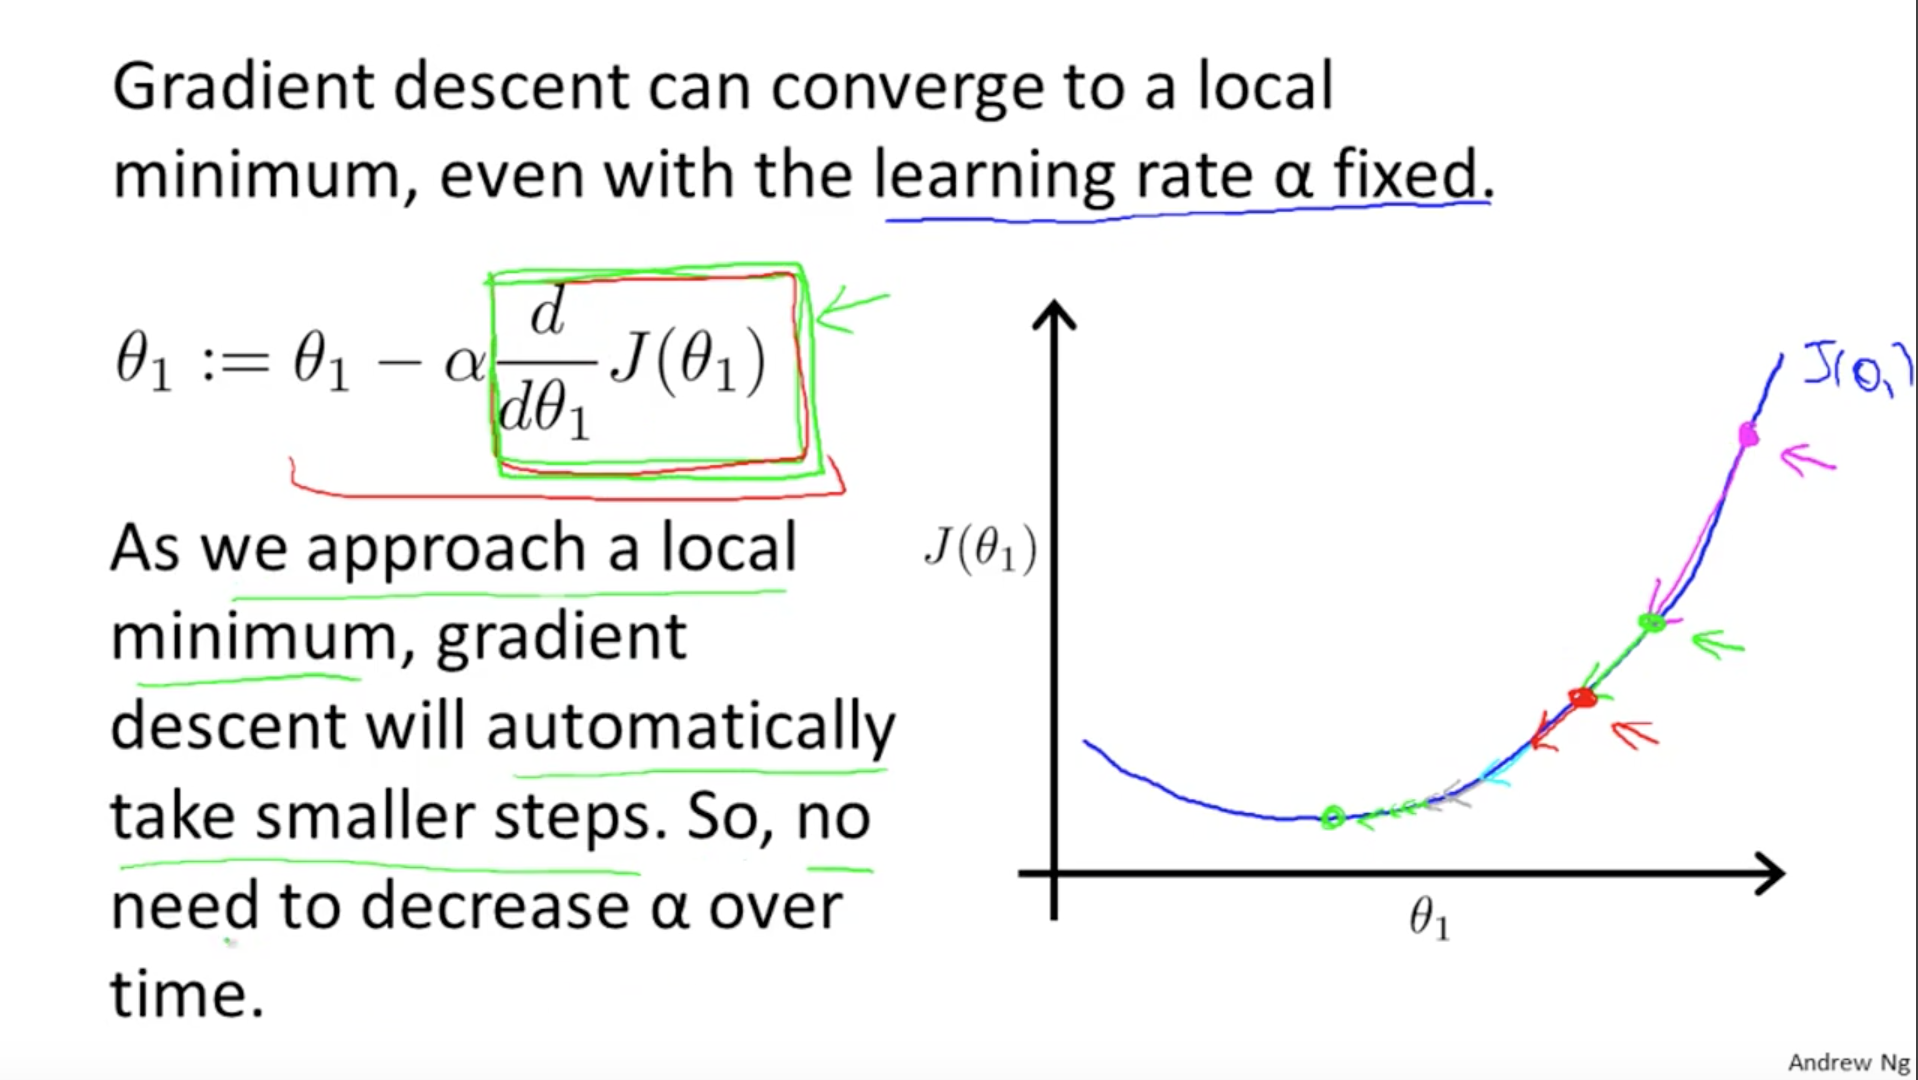
\includegraphics[width= 1.5\textwidth,center]{intuition_on_gradient_descent.png}
		\caption{By taking the negative of the derivative, we know which way to go to move towards the global minima}
	\end{figure}
	\item (note: thinking about it further, gradient descent really does seem like newton's method. I'll have to fact check that later.)
	\item To elaborate on the alpha, the alpha can be thought of as the "step size" of gradient desc.
	
	\item the equation for this cost function is:
	\item $J(\theta)=\frac{1}{2m}\sum\limits_{i=1}^{m}(h_\theta(x^{(i)})-y^{(i)})^2$
	\item 
\end{itemize}

\begin{itemize}
\item note: to "normalize" or "keep the 'features' in the same range so that gradient descent will flow more naturally"  subtract the mean value, and divide by the standard deviation
\item also, if you normalize the features, when you test your resulting function, normalize the input first. Because you normalized the test data, the function is set to work for normalized values. (and use the same mean and standard deviation)
\end{itemize}

\section{Gradient Descent (something like Newton's Method)}
\begin{itemize}
	\item basically partial derivative of Cost Function $J(\theta)$ with respect to each $\theta$
	\item accidentally already explained this in the previous section.
	\item But to continue, we can also do multivariate linear regression, where we just have more theta's and more variables (nothing new)
\end{itemize}

\section{Using Matrix Normalization to Find the Optmial Theta Parameters}
	\begin{itemize}
		\item include equation $ (X^T*X)^{-1}*X^T*y$
		\item what to do when $X^T*X$ is non invertible?
		\item in Matlab, use pinv
		\item remove redundant features (for example, there are two parameters for the same measurement, but in feet and meters)
		\item there could be too many features
	\end{itemize}

\section{Logtistic Regression or "Classification"}
\begin{itemize}
	\item used for classifying things (like spam/not spam)
	\item $ h_{\theta}(x) = g(\theta^T*x)$
	\item where sigmoid/logistic function $g(z) =\frac{1}{1+e^{-z}}$
	\item $ h_{\theta}(x)=\frac{1}{1+e^{\theta^{T*x}}} $
\end{itemize}

\section{Overfitting (the function tries too hard to fit the training data and does not make a general equation)}
\begin{itemize}
\item Reduce number of features
	\begin{itemize}
		\item Manually select useful features
		\item Model section algorithm (to pick features automatically)
		\item Hard to say if features are all needed or not
	\end{itemize}
\item Regularization
	\begin{itemize}
		\item Keep features, reduce magnitude of $\theta_j$, perhaps keep to -0.03 range to 0.03
		\item Works well when many features exist
		\item Small values for theta parameters gives "simpler" hypothesis, less prone to overfitting
		\item choose a good $\lambda$
		\item Regularized linear regression: $J(\theta) = \frac{1}{2m} [ \sum\limits_{i=1}^{m} (h_{\theta}(x^{(i)}) - y^{(i)})^2 + \lambda \sum\limits_{j=1}^{n} \theta_{j}^{2} ]$
		\item Can use algorithm to automatically chose $\lambda$ as well
		\item Regularized Gradient Descent: (Don't regularize $\theta_0$)\\
		Repeat \{\\
		$
		\theta_0 := \theta_0 - \alpha \frac{1}{m} \sum\limits_{i=1}^m (h_{\theta}(x^{(i)}) - y^{(i)})x_0^{(i)}\\
		\theta_j := \theta_j - \alpha [ \frac{1}{m} \sum\limits_{i=1}^m (h_{\theta}(x^{(i)}) - y^{(i)})x_j^{(i)} + \frac{\lambda}{m}\theta_j ]$\\
		\}
		
		\item the second theta eqn can be simplified to $\theta_j := \theta_j(1 - \alpha\frac{\lambda}{m}) - \alpha \frac{1}{m} \sum\limits_{i=1}^m (h_{\theta}(x^{(i)}) - y^{(i)})x_j^{(i)}$
		\item $\alpha$ is usually small, there are many training examples (large m),  so that usually results in a small value
		\item Note, a large $\lambda$ can result in underfitting, and a small one results in overfitting
	\end{itemize}
\end{itemize}

\section{Normal Equation after regularized}
	\begin{itemize}
		\item deriving cost function wrt theta and setting it = 0 results in normal equation
		\item after regularizing this results in a similar equation, but with adding lambda times a identity matrix with the first element being set to 0 in the inverting part of the equation (this identity matrix being (n+1) by (n+1))
		\item if this lambda is greater than 0 then the matrix to be inverted will never be "singular" or uninvertable
		\item there is an advanced optimization part in the second assignment pdf. it uses fminunc (f min unconstrained). read more there. (remember to use @costFunction for using your costFunction )
	\end{itemize}
	
\section{Non-Linear Classification \& Neural Networks}
	\begin{itemize}
		\item when you have lots of features, and you need to have them become higher order, there might bee too many items
		\item so logistic and linear regression doesn't quite work as quickly as it would on a smaller feature problem
		\\
		\item We can use a Neuron Model: Logistic unit
		\item We have "dendrites" (the inputs) the cell body (the function) and the output (our hypothesis or the axon)
		\item still have x's and parameters. Note that the prof sometimes adds x0 or a0 as a bias unit
		\item a Neural network can be represented by "layers", like input layers, fed into a "hidden" (neurons) (anything not input or output layer) layer, fed into an output layer (our hypothesis)
		\item the dimensions of this $\theta^{(j)}$ are $s_{j+1}x(s_j + 1)$, meaning the size/number of units in the next layer by the number of units in the current layer plus 1 (ex. 2 inputs, 4 neurons, so 4 x 3 theta parameter) 
		\item for our course at least, the super scripts will mean which layer the item came from.
		\item subscript will be which item in the layer
		\begin{figure}[ht!]
			%\centering
			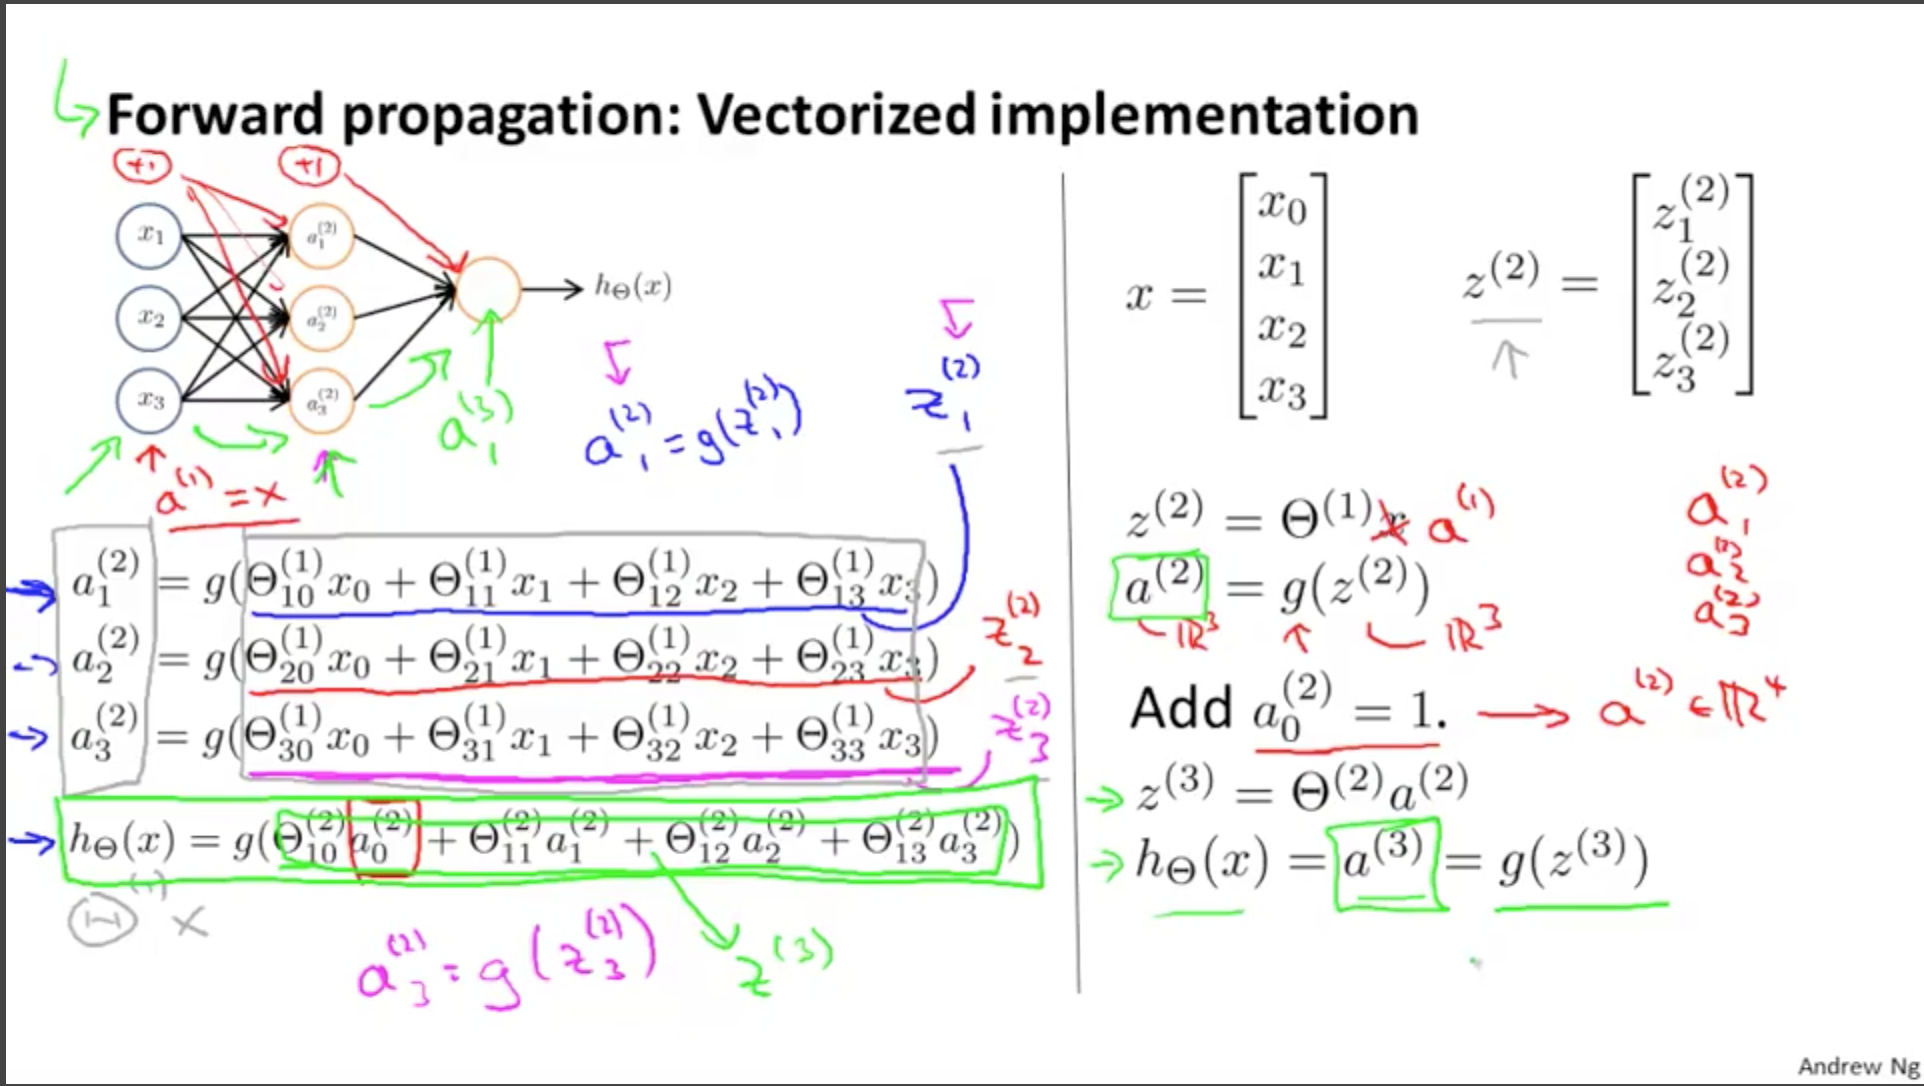
\includegraphics[width=1.5\textwidth,center]{Forward_Propogation_and_Vectorization.png}
			\caption{A general neural network. Vectorization of the code makes it faster, especially using a gpu to handle the computations in parallel}
		\end{figure}
		\item neural networks are like logistic regression, except, instead of using x inputs, it uses it's own learned inputs. the inputs (x's) are fed into it's a's, which are it's own inputs, which are then fed into a logistic regression layer.
		
		\item we still use J of theta and the derivative wrt theta
		\begin{figure}[ht!]
			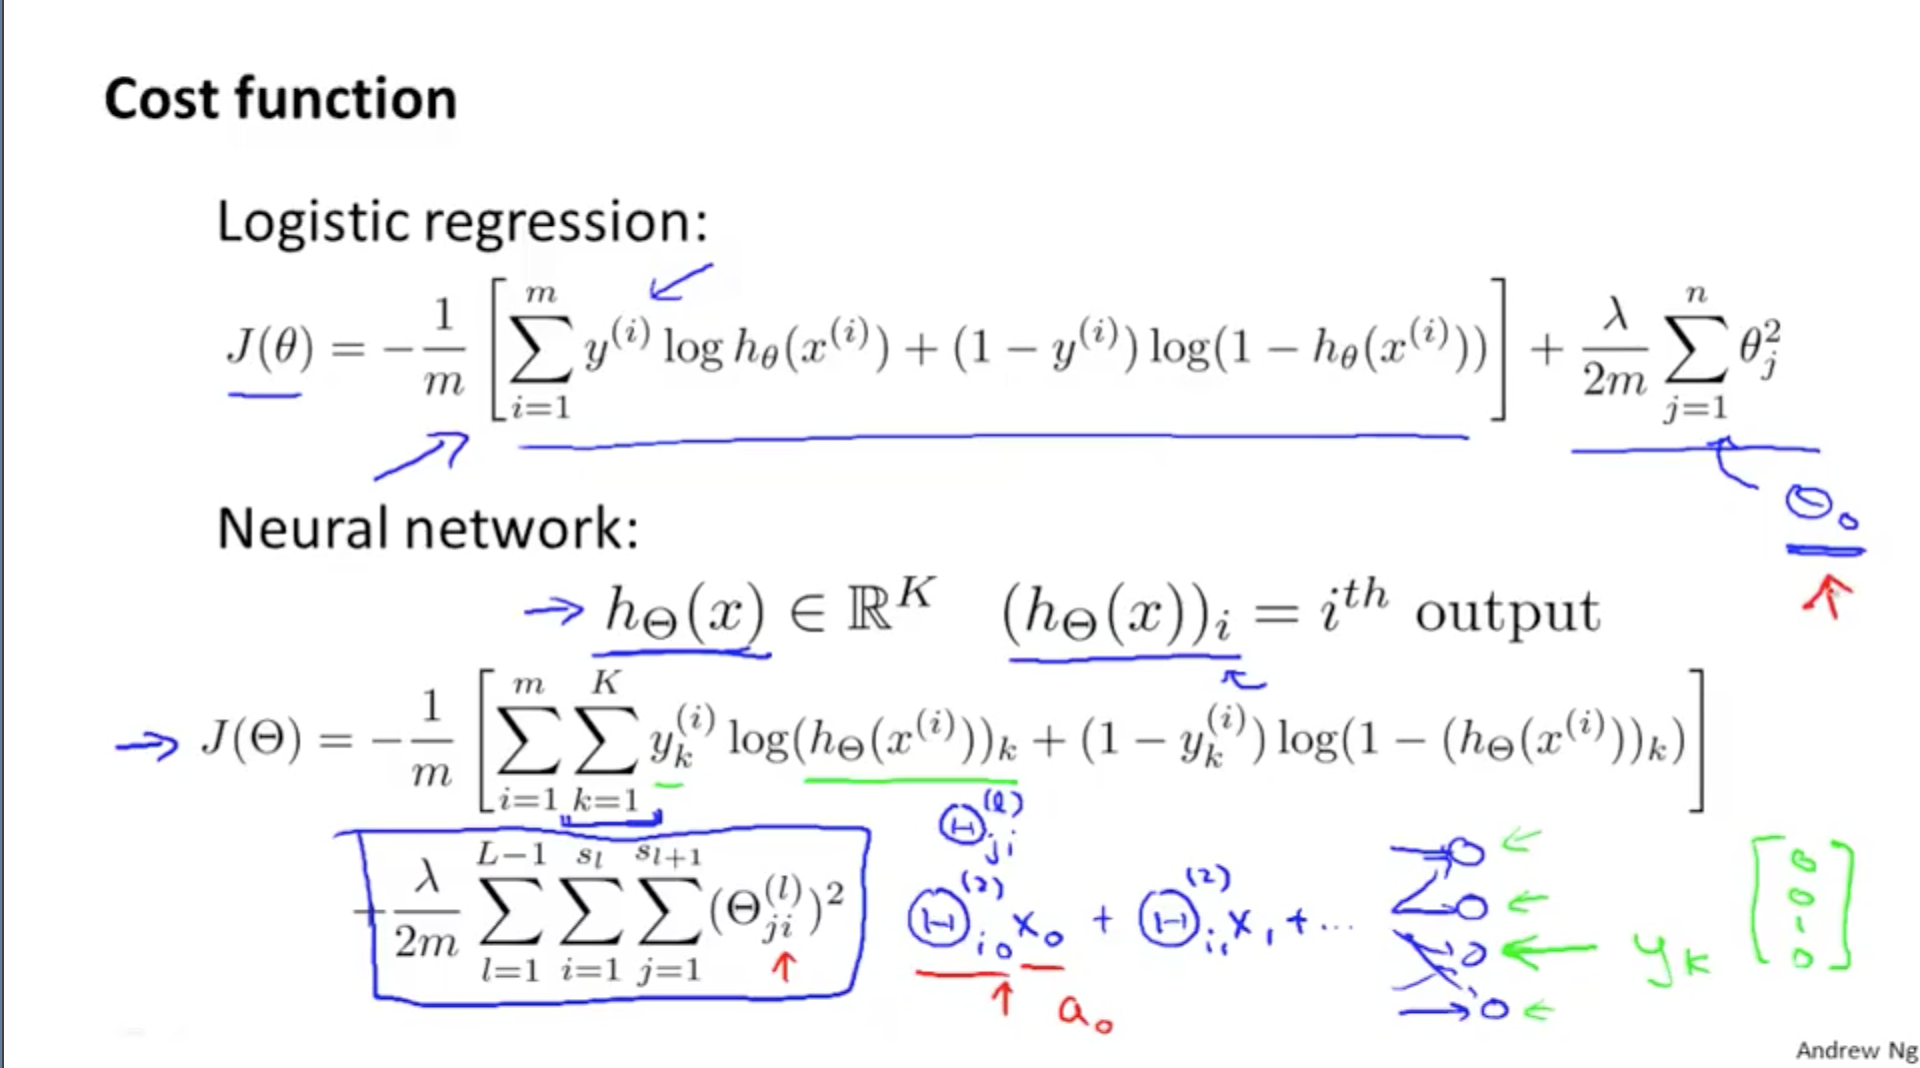
\includegraphics[width= 1.5\textwidth,center]{Cost_Function_neural_net.png}
			\caption{The cost function for a neural net.}
		\end{figure}
		
		\begin{figure}[ht!]
			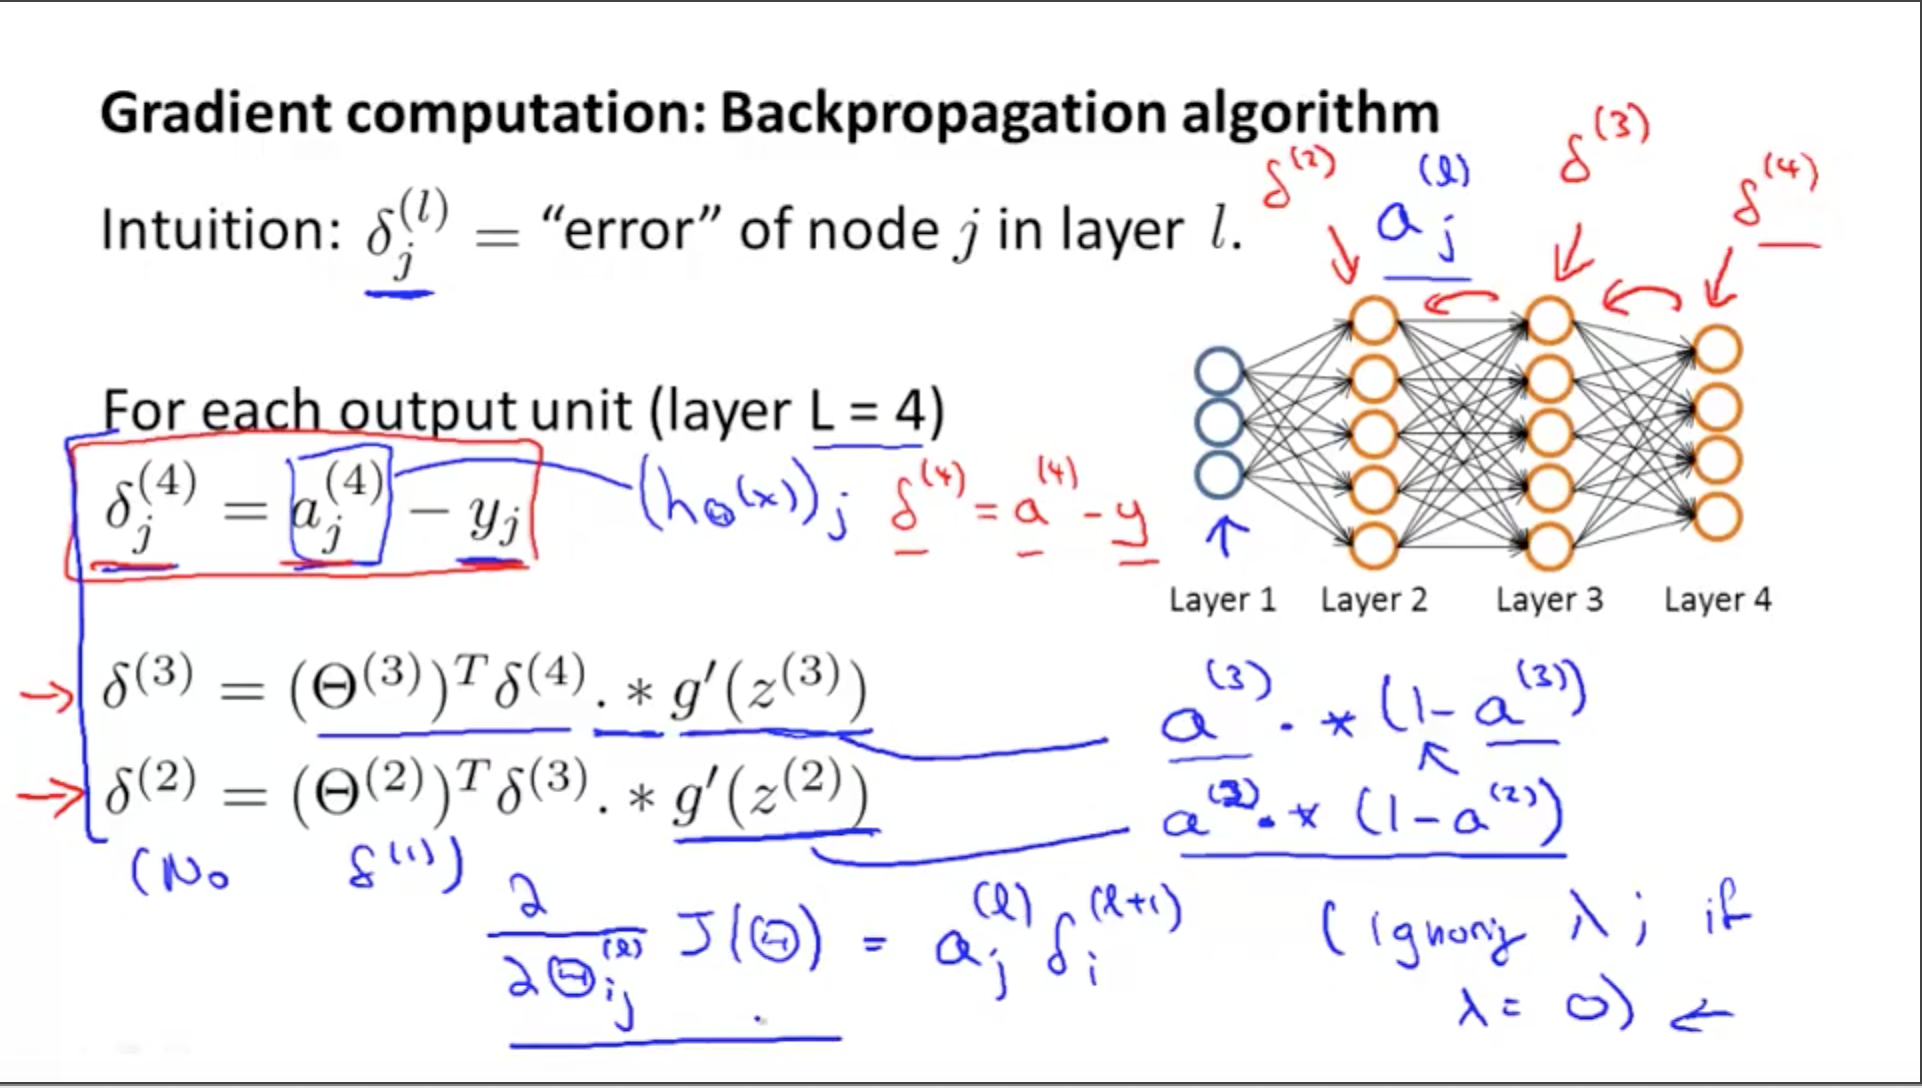
\includegraphics[width= 1.5\textwidth,center]{delta_error_term.png}
			\caption{There is a error term, shows how far off we are. Reminds me of calculus class, with the error term of a Taylor/Mclaurien Polynomial}
		\end{figure}
		
		\clearpage
		
		\item We use forward propagation to get our $z^{(2)} = \theta^{(1)}a^{(1)}$ and $a^{(2)}= g(z^{(2)})$ (and eventually our hypothesis)
		\item We use backwards propagation to get our $\delta$(kinda like in calculus with the error term in a Taylor Polynomial)
		\item We can unroll our theta's into one large theta vector, and also do the same for D (delta).
		\item In Matlab/Octave, we can use the reshape() function to get back our vectors
		
	\end{itemize}
	
	\subsection{Numerical Gradient Checking - make sure there aren't those subtle errors in your program!}
		\begin{itemize}
			\item Basically a little bit of that $\epsilon$/$\delta$ or the general calculus derivative with the f(x+h) - f(x) / h, but we also subtract h from the second term. (so the one I knew was one-sided, but this one is two-sided and more accurate)
			\item Only use Gradient Checking for testing to make sure there isn't an error in the program code
			\item When actually implementing, use backprop (backpropagation) for learning
		\end{itemize}

	\subsection{Choosing the Initial Value of $\theta$}
		\begin{itemize}
			\item While just using a vector full of zeros works for the previous algorithms, it doesn't work for Neural Nets.
			\item If they're zero, then at the layer after the input layer, then $a_1^{(2} = a_2^{(2)}$, the terms will both be the same due to this theta of zeros, the delta ($\delta$) values will be the same as well and the $\theta$ will be the same (same meaning theta1 and theta2 equal to eachother).
			\item So, we have \emph{Random Initialization}! We need to pick random values for theta, as well as \emph{breaking symmetry}. 
			\item To break symmetry we init each theta to a random value in $[-\epsilon,\epsilon]$. We make a rand(x,y) random matrix of size x by y, multiply by 2 times $init_\epsilon$, and then subtract this $init_\epsilon$, and now we have one of our thetas.
			
		\end{itemize}
		
	\subsection{Training a Neural Network}
		\begin{itemize}
			\item Pick a network architecture (a pattern between neurons. like 3 inputs, 5 neurons in the second layer, and 4 output hypotheses)
			\item \# of input units: Dimension of features $x^{(i)}$
			\item \# of output units: Number of classes (could be 1-10 like the numbers from MNIST)
			\item Reasonable \# default: Just use 1 hidden layer. Or, if > 1 hidden layer, use same \# of hidden units in every layer (the more the better)
			\item \# of hidden units usually should be comparable to \# of input units or features, maybe even 2x, 3x ... 7x the \# of input units
			
			\begin{enumerate}
				\item Randomly init weights (parameters/$\Theta$s)
				\item Implement forward propagation to get $h_\Theta(x^{(i)})$ for any $x^{(i)}$
				\item Implement code to compute cost function $J(\Theta)$
				\item Implement backprop to compute partial derivaties $\frac{\partial}{\partial \Theta_{jk}^{(l)}}J(\Theta)$
				
				\begin{enumerate}		
					\item could use for loop and do fp and bp at each layer, but you can vectorize it (they say it's advanced, but let's see about that)
					\item in the for loop, also get activations $a^{(l)}$ and delta terms $\delta^{(l)}$ for $l=2,...,L$ ($l$ being the current layer that we iterate through with the for loop and $L$ being the last layer number)
					\item something like $\Delta^{(l)}:=\Delta^{(l)} + \delta^{(l+1)}(a^{(l)})^T$
					\item after the for loop, compute the partial derivative terms of the cost function J
				\end{enumerate}
				
			\item Use gradient checking to compare $\frac{\partial}{\partial \Theta_{jk}^{(l)}}J(\Theta)$ computed using backpropagation vs. using numerical estimate (the $\epsilon$ thing) of $J(\Theta)$.
			\\Then disable gradient checking code
			\item Use grad descent or an advanced optimization method (with fminunc) with backpropagation to minimize J
			\item This $J(\Theta)$ is non-convex (not a bowl) and can get stuck on local minima (unlikely, but could happen).
			
			\end{enumerate}
			
		\end{itemize}
		
	\section{Debugging a Learning Algorithm}
		\begin{itemize}
			\item What should you do if your trained hypothesis makes errors in it's predictions?
			\item > Get more training examples
			\item > Try a smaller set of features (prevent overfitting)
			\item > Try more/better features
			\item > Add polynomial features (Try visualizing first, and try to guess which polynomial would look good)
			\item > increase or decrease $\lambda$
			\\
			\item Try running a Machine Learning Diagnostic
			\item It takes time to make and understand, but can be very informative as to what to improve
			\\
			\item Try Visualizing the hypothesis
			\item (better used if we have multiple feature training sets)
			\item But we can still Evaluate the Hypothesis by splitting a training set into parts
			\item We can assign 70\% of the training set as the training set, and 30\% as the test set
			\\
			\item Training/Testing Procedure for Linear Regression
			\item > Learn $\theta$ from training data (minimize J, for that 70\% of the training set)
			\item > Compute test set error J for our test set 30\%
			\\
			\item Training/Testing Procedure for logistic Regression
			\item Learn $\theta$ from training set
			\item Compute test set error J for logistic regression
			\item Check for Misclassification error (0 or 1)
			\item err($h_\theta^{(x)},y$)= 1 if it's greater than 0.5 and y = 0 then there's an error , 0 otherwise
			\item basically check if there's an error
			\item comes out to be test error = 1/m(test) * sum(err($h_\theta(x_{test}^{(i)})$)) from i=1 to m(test)
			\\
			\item Model Selection
			\item Evaluating your hypothesis
			\item set 60\% to training set, 20 to cross validation set, 20 to test set
			\item Now we can define error J for training, cost validation, and test error with the same J eqn we've used
			\item Now test different order hypotheses on the cross validation set, and pick the best/lowest J eqn from the different order hypotheses
			\\
			\item Choosing regularization parameter $\lambda$
			\item try different values of lambda, could try doubling lambdas, then check the J value for the best J
			\item Note: getting more training data is helpful when there's high variance or Jcv is >> than Jtrain
			\\
			\item Note: high bias: hypothesis is too simple (underfitting) hypothesis, training data not fit well (J for training and test both high)
			\item add more features, training, 
			\item Note: high variance: hypothesis is too complex, overfitting hypothesis,
			\item less features, adding data won't help
			\\
			\item Remember, a high lambda will make the thetas worth less, kinda like removing those features (can underfit and cause high bias, or fix high variance), and a low lambda will make the thetas worth more, like emphasizing them (can make over fit and cause high variance, or fix high bias)
			\item note: if there's high bias, only adding training examples might not help, since it could be that lambda is too large so our thetas are being penalized and shrunk to approximately zero
			\item note: if there's hight variance, adding more examples can help since the model is overfitting the training data. Adding more training data will increase the complexity of the training set which makes it harder for the hypothesis to force some kind of weird function that will fit the training examples
			\item note: to get this visualization, we can graph the error J for test and training sets Vs. the m training set size.
		\end{itemize}
	
\section{Prioritizing What to Work on - Less Math, Mostly Plain Old Logic}

	\subsection{Example: Building a spam classifier}
		\begin{itemize}
			\item We could take a look at the different words used, like buy, deal, discount, etc.
			\item From this, we could have a vector of 1's and 0's to show which words exist in this email.
			\item For this example, we could pick 100 words
			\item In practice we could check for the most frequently occurring n (10k to 50k) words
			\item Now, collecting lots of data might help, or not.
			\item We can make sophisticated features based on things like the email's routing (address, header, etc.)
			\item Have sophisticated features to maybe count "discount" and "discounts" as the same word
			\item Have algorithm to detect misspelled words, like w4tches, m0rtgage, etc.
		\end{itemize}
		
	\subsection{Error Analysis}
		\begin{itemize}
			\item Start with a simple algorithm that can be implemented quickly and tested on the cross-validation data (quick and dirty, could be a little bit longer that "quick")
			\item with this, plot learning curves to decide if you need more data, features are likely to help by checking for high bias or variance, AND AVOID THE ROOT OF ALL EVIL THAT IS PREMATURE OPTIMIZATION (Ahem, sorry, got a little carried away there)
			\item this evidence is more useful than going with a gut feeling and falling prey to premature optimization
			\item Check  training examples in cross validation set that your algorithm makes errors on, check for any trends
			\item Ex. the spam classifier, manually check the types of the emails, features that would have helped to have
			\item could categorize emails into specific categories like stealing passwords, pharma, fakes, etc.
			\item could check \# of occurrences of deliberate misspellings, unusual email routing, unusual punctuation, and focus making features on those specific metrics
			\item Remember, a quick and dirty implementation is good for checking what might be good leads to follow
		\end{itemize}
		
	\subsection{The importance of numerical evalutation}
		\begin{itemize}
			\item Ex. the spam: should discount/discounts/discounted/discounting be treated as the same word?
			\item Use "stemming" software?
			\item but it could make mistakes like universe/university
			\item Best way? Use it and observe the results for signs of success/failure (higher or lower error percent?)
			\item Another issue: lowercase vs uppercase (Mom/mom), again, implement then check error
			\item Rule of thumb: test your idea first, then check the error for improvements
			\item and remember, test this on the cross validation set, not the test set, you don't want to train the algorithm to be good at the test set!
		\end{itemize}
		
	\subsection{Error Metrics for Skewed Classes}
		\begin{itemize}
			\item Cancer classification example
			\item lets say you have only 1\% error on the test set
			\item BUT only 0.5\% have cancer. we have skewed classes since we have a small group of positive data in out data set
			\item Say we made a change and now our error improved by 0.3\%, did we do something useful?
			\item hard to say with this skewed data set. we might have just made our algorithm predict zero more often
			\item we should check the precision of our algorithm.
			\item Precision = $\frac{True +ve}{\# predicted postitive} = \frac{True +ve}{True +ve + False +ve}$
			\item Now Recall, \# of patients with cancer Vs. our predicted amount
			\item Recall = $\frac{True +ve}{\# actual postitive} = \frac{True +ve}{True +ve + False -ve}$
			
			\begin{figure}[ht!]
				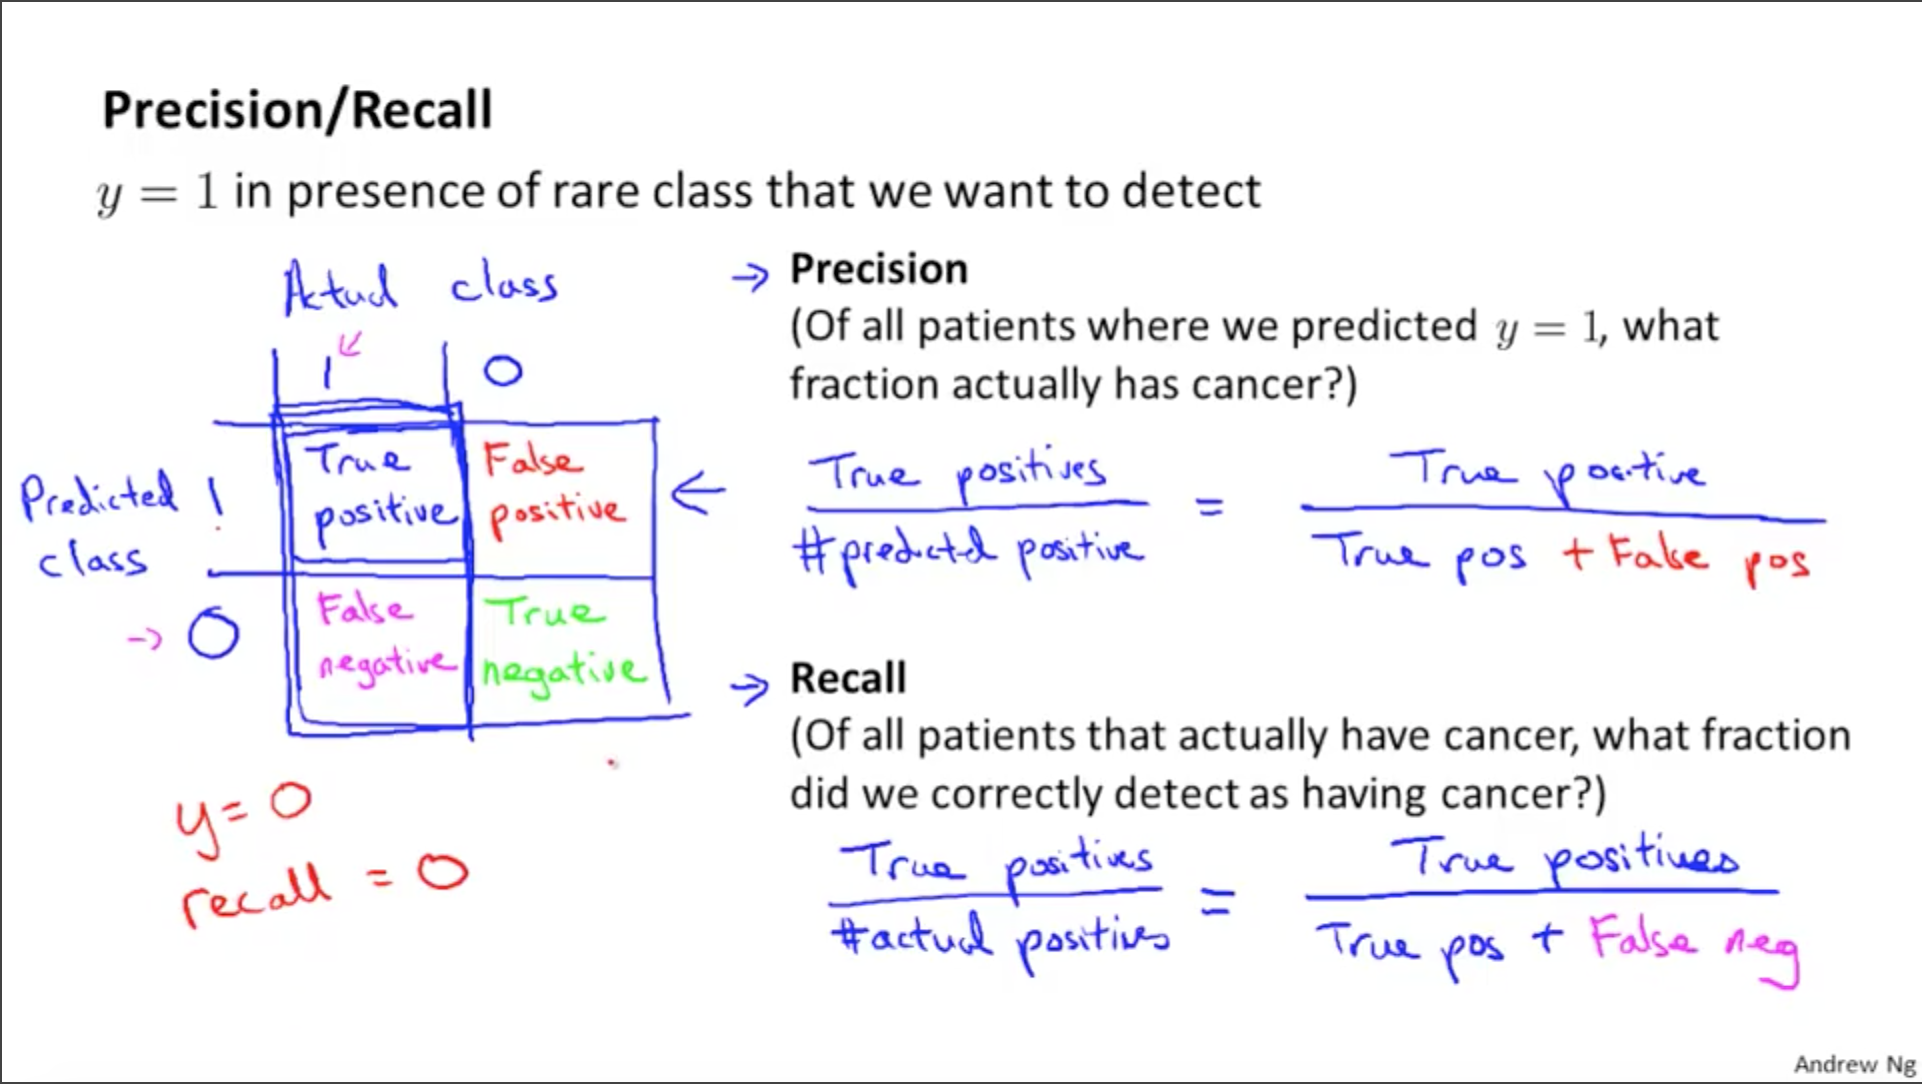
\includegraphics[width= 1.5\textwidth,center]{Precision_and_Recall.png}
				\caption{Precision and Recall.}
			\end{figure}
			
			\item Note: Accuracy is just true +ve plus true -ve divided by total examples
		\end{itemize}
		
	\subsection{Trading off precision and recall}
		\begin{itemize}
			\item continuing on the cancer example
			\item how about changing our logistic regression to output 1 if our hypothesis is greater than 0.7 to try to ensure we have a high confidence in our prediction
			\item This gives higher precision, but lower recall
			\item But then true positive cases might slip by
			\item If we want to avoid missing these cases we could change the threshold again! maybe to something like 0.3
			\item This gives lower precision, and higher recall
			\item We can make a graph with different thresholds and make a decision with it!
			\item let's check the (P)recision and (R)ecall for different thresholds, and take the F score of them, and pick the best settings based on it!
			\item $F_1 Score = 2\frac{PR}{P+R}$
			\item Note: bad F score -> P and R both = 0, so F = 0, where as a good one will have them all equal 1
		\end{itemize}
		
	\subsection{Data for Machine Learning}
		\begin{itemize}
			\item Designing a high accuracy learning system
			\item Ex.
			\item Let's say we have enough data for feature X for a good prediction
			\item Counter Ex. Predict housing prices with just X (Not a good thing to try)
			\item Thus, try a little useful test, where a human expert predicts y using X. If they can do it, then a computer should be able to do it too.
			\item Rationale Behind Large Data
			\item Ex use learning algorithm  with many params, (regression with many features or neural networks with many hidden units)
			\item With a large training set, we are unlikely to have overfitting bias, so we can have low variance.
			\item Lesson: Have good features (one a human could use as well) and a decently sized training set.
		\end{itemize}
	
	\subsection{Support Vector Machines}
		\begin{itemize}
			\item Let's start by looking at logistic regression
			\item In it's cost function, when y = 1, the (1-y) term disappears. And when the z is greater than zero the value gets smaller
			\item To build a SVM from this, we just have an approximation of the cost function and break it into two pieces
			%image here
			\begin{figure}[ht!]
				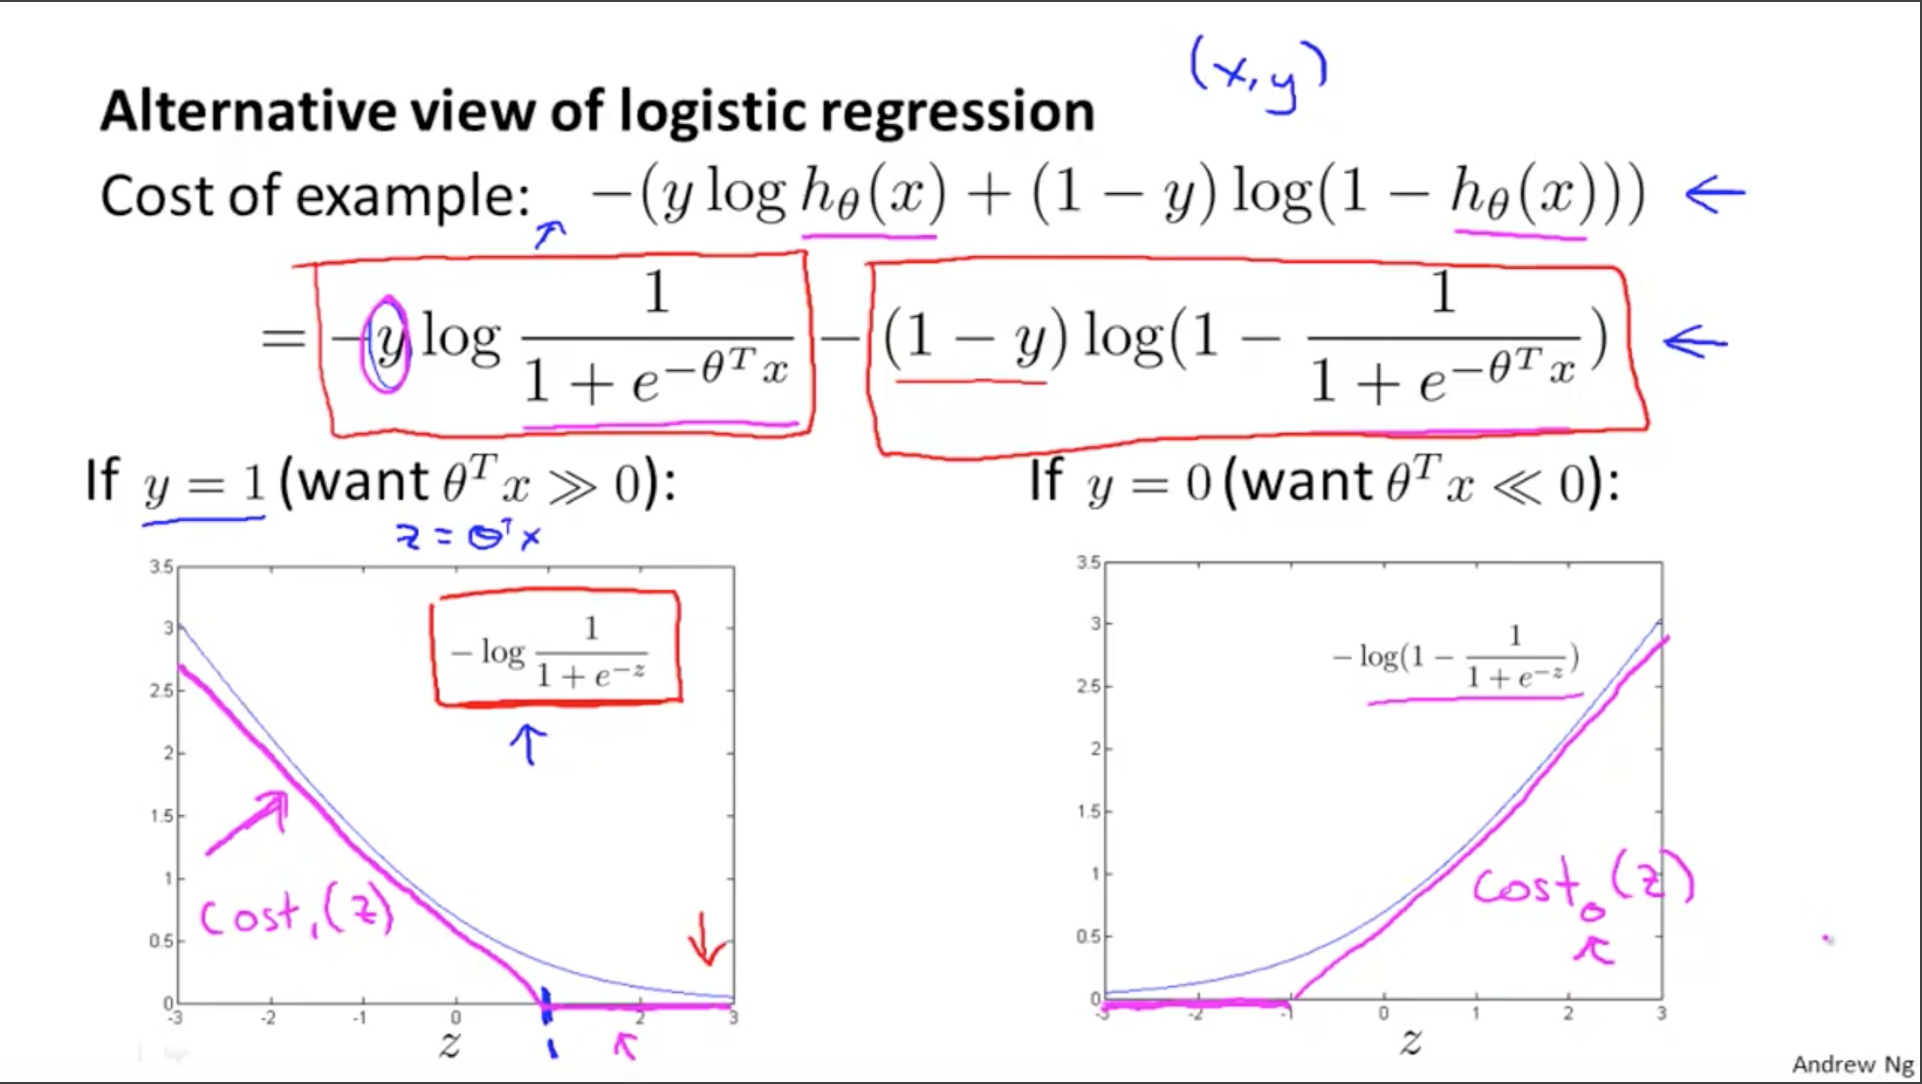
\includegraphics[width= 1.5\textwidth,center]{SVM_From_Logistic.png}
				\caption{Get SVM from Logistic Regression.}
			\end{figure}
			
			\item In other words, we can replace the -log h terms with cost1 and cost0
			\item we will also remove 1/m from the cost J and regularization parameter lambda since it's just a constant
			\item we can also scale them by setting a constant C = 1/m, and also C = 1/lambda
			%image here
			\begin{figure}[ht!]
				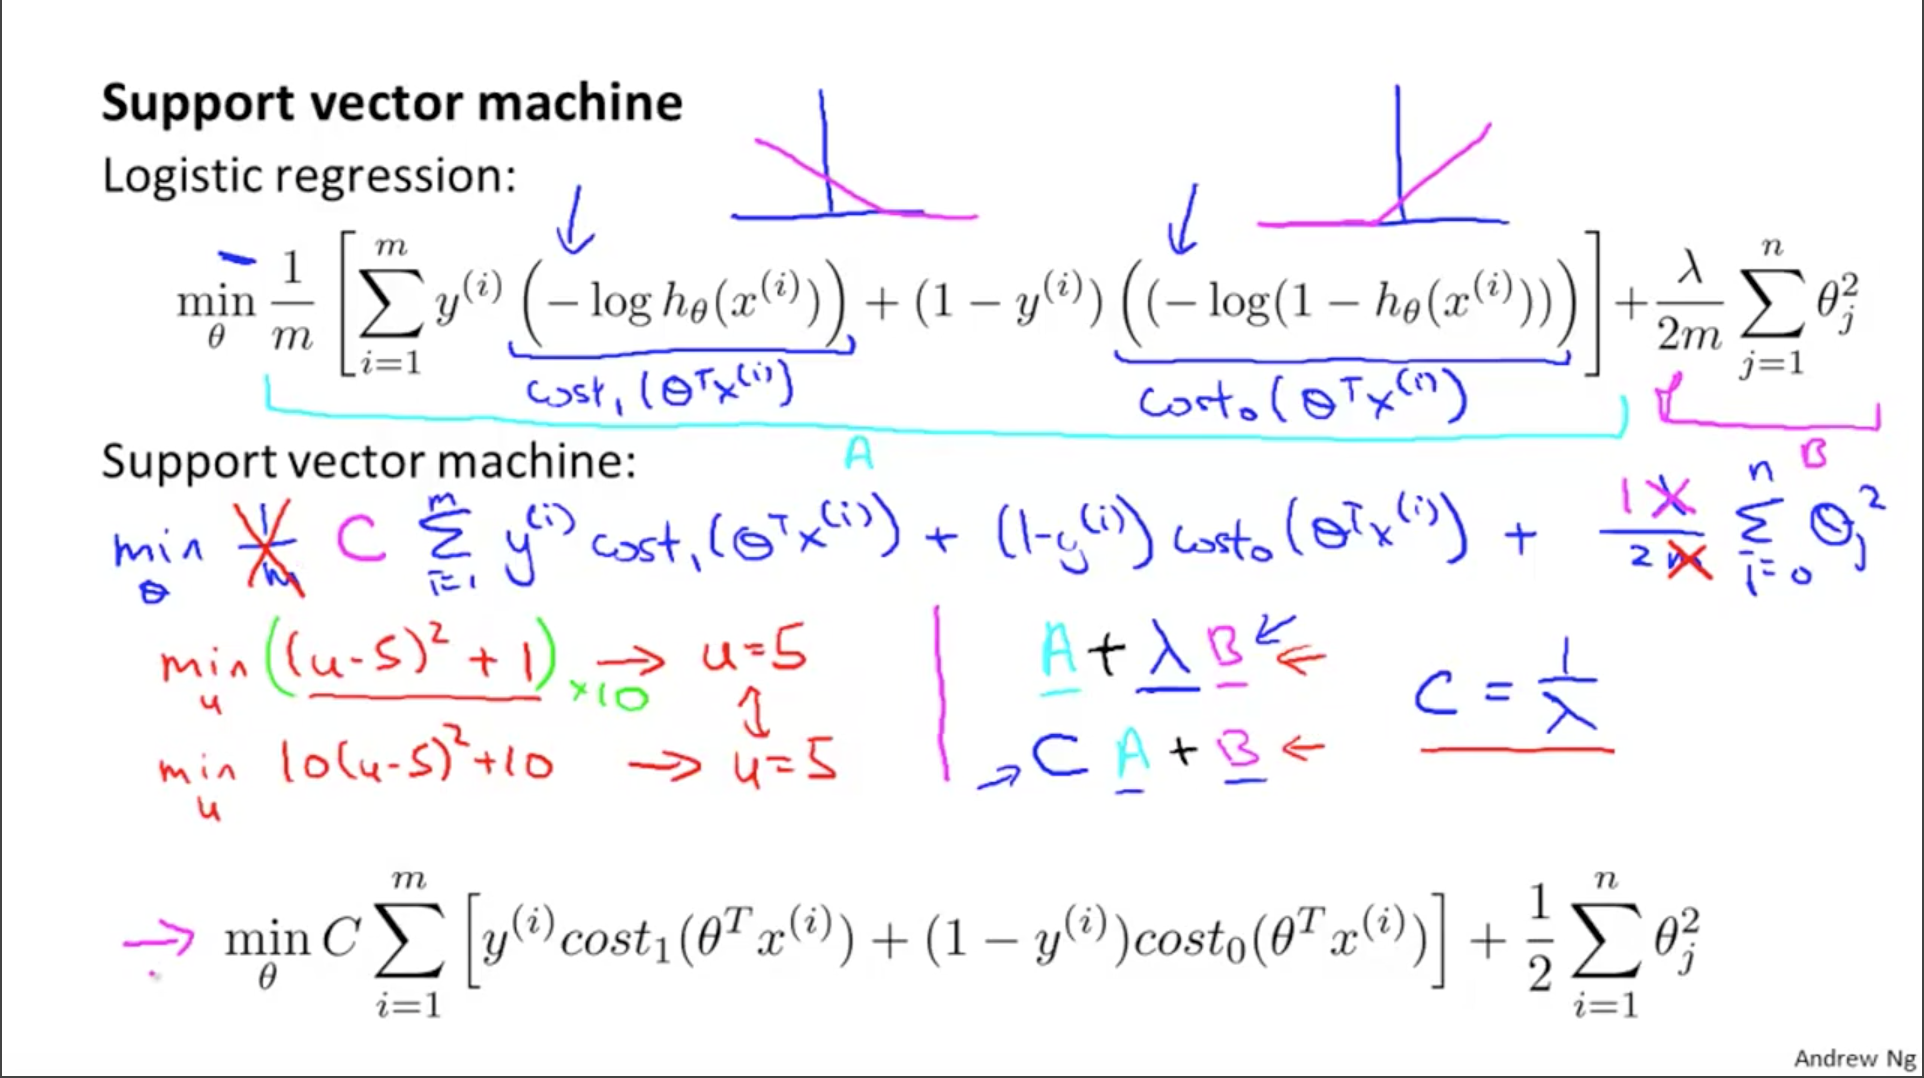
\includegraphics[width= 1.5\textwidth,center]{Constant_C.png}
				\caption{C is 1/m and 1/lambda.}
			\end{figure}
			
			\item Note: SVM doesn't predict probability, it predicts 0 or 1, a true or false
			\item h = 1 if $\theta^Tx >= 0$ and h = 0 otherwise
			\item making constant C a light number, the summed part goes to zero
			\item Note: when calculating the cost, for y = 1, we want to try to get theta times x to be >= 1 since this would get a 0 from the cost function of our SVM, and vice versa for y = 0
			%include last 3 images
			\begin{figure}[ht!]
				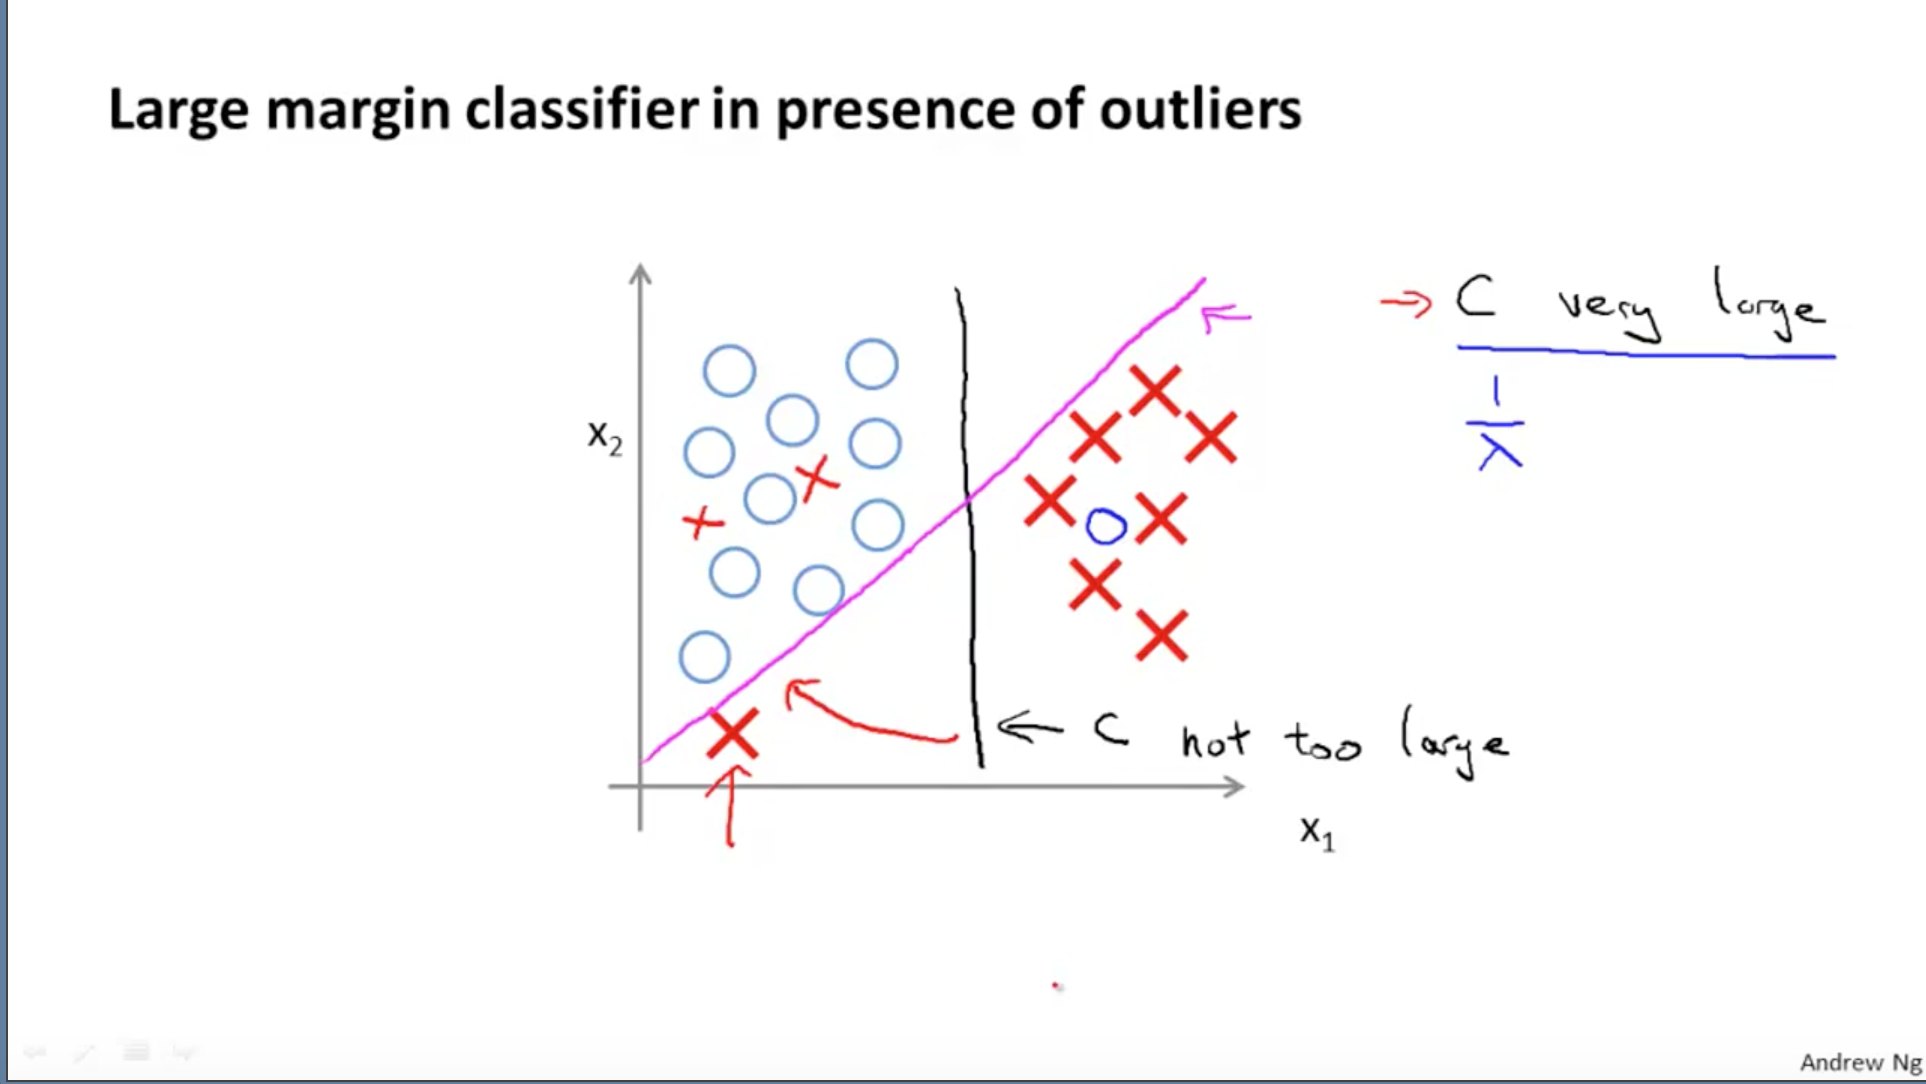
\includegraphics[width= 1.5\textwidth,center]{Theta_X_Value.png}
				\caption{Some explanation on how it works.}
			\end{figure}
			
			\item note: to make this SVM decision boundary, the intuition to follow is that it tires to maximize the vector projection projected by each testing data point, and create the largest margin
			% include last 4 images
			\begin{figure}[ht!]
				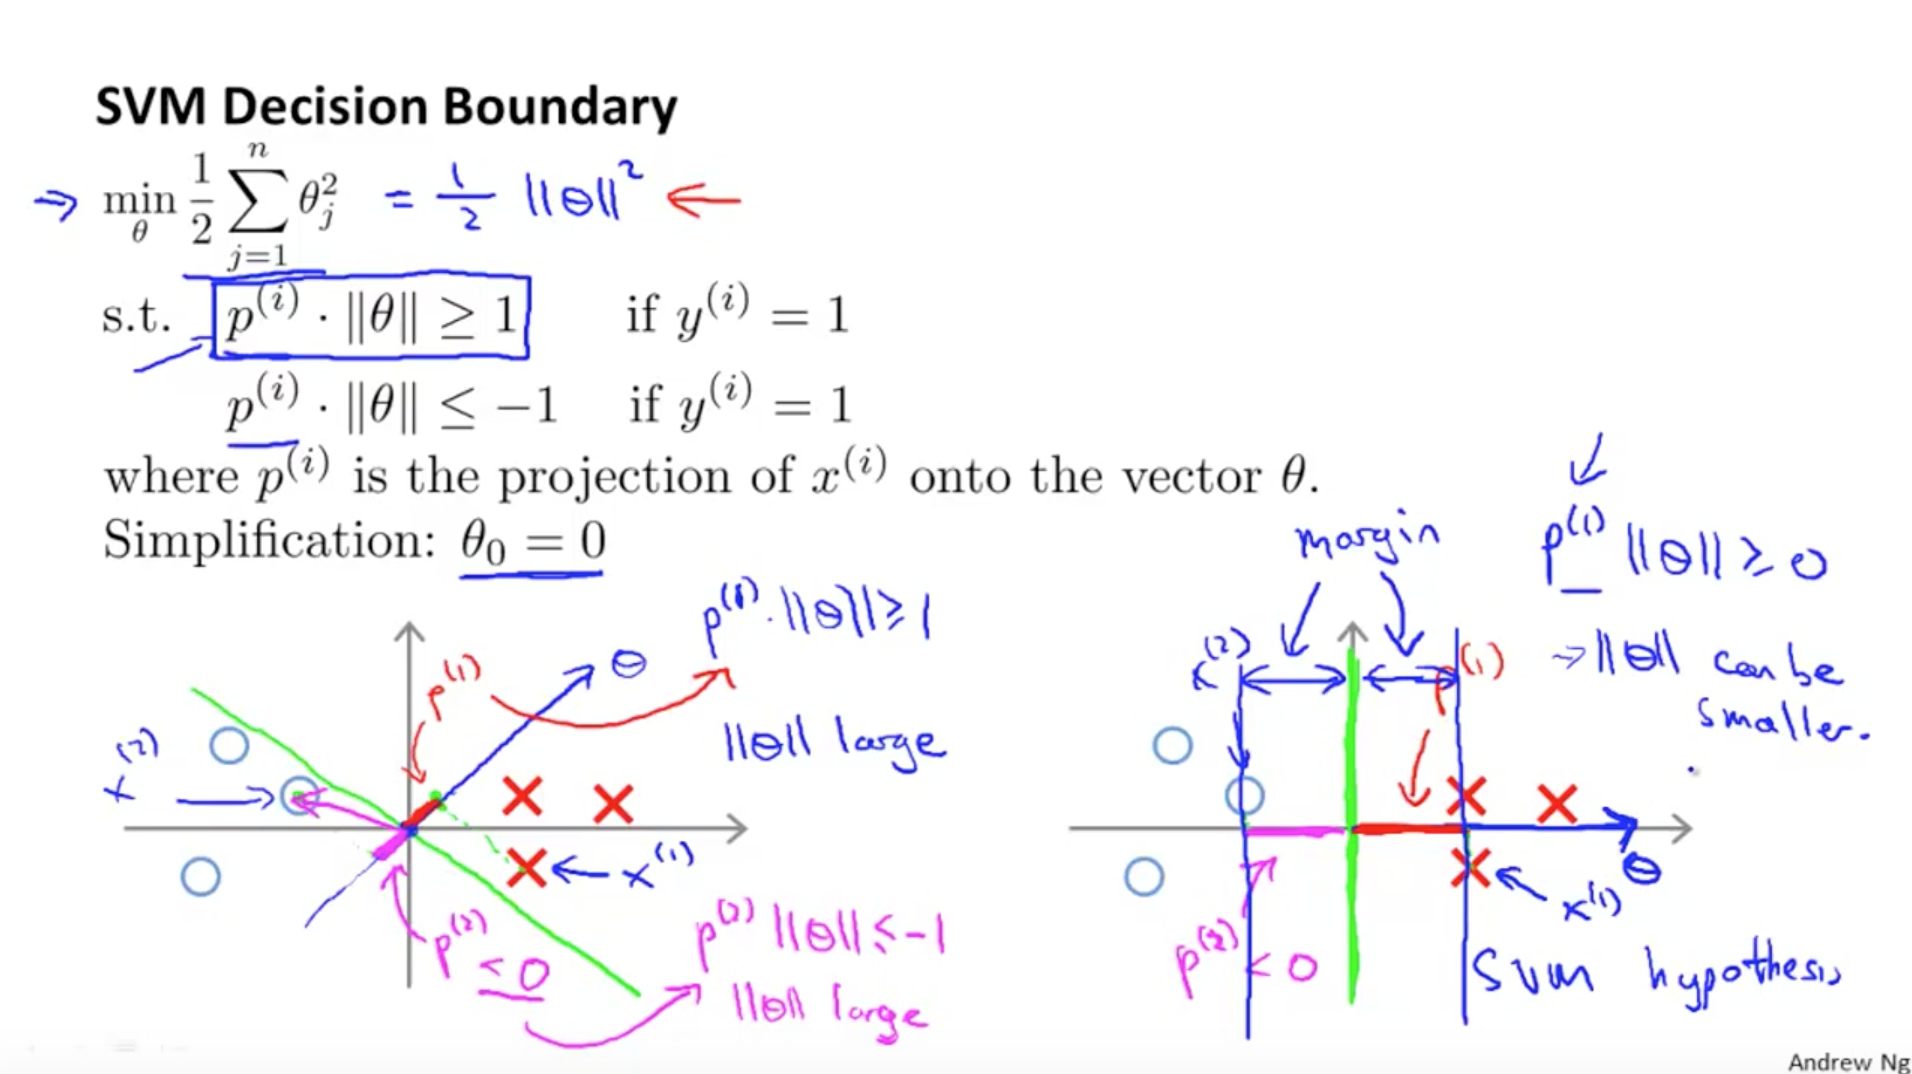
\includegraphics[width= 1.5\textwidth,center]{SVM_Intuition.png}
				\caption{Intuition on SVM.}
			\end{figure}
		\end{itemize}
		
	\subsection{Kernels}
		\begin{itemize}
			\item With non-linear decision boundaries, we usually have had polynomial features
			\item But is there a better feature set to use?
			\item We can use x to compute new features depending on proximity landmarks
			\item We calculate kernels of similarity of x and landmarks l, with the eqn $e^{-\frac{\| \mathbf{x-\ell} \|^{2}}{26^2}}$ (this eqn is a Gaussian kernel)
			\begin{figure}[ht!]
				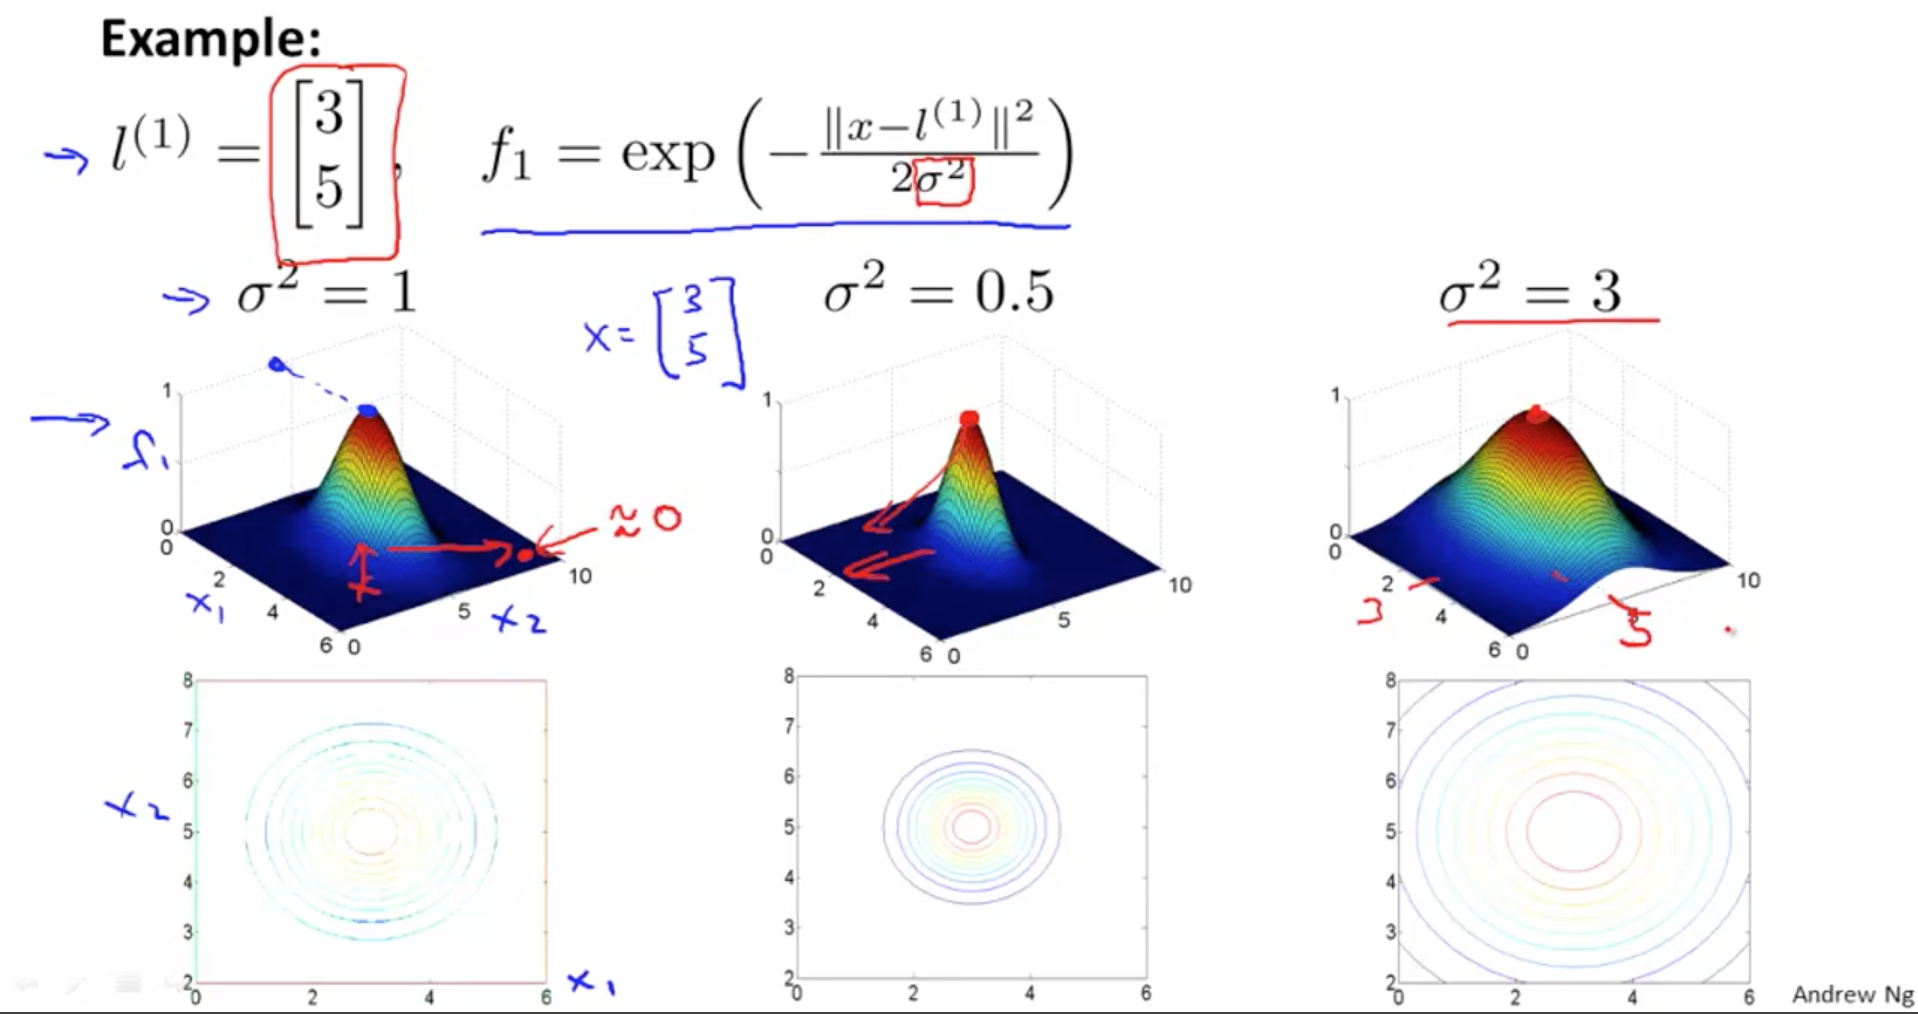
\includegraphics[width= 1.5\textwidth,center]{Kernel_Features.png}
				\caption{Kernel feature.}
			\end{figure}
			\item Cute trick with calculating the regularization term with theta
			\begin{figure}[ht!]
				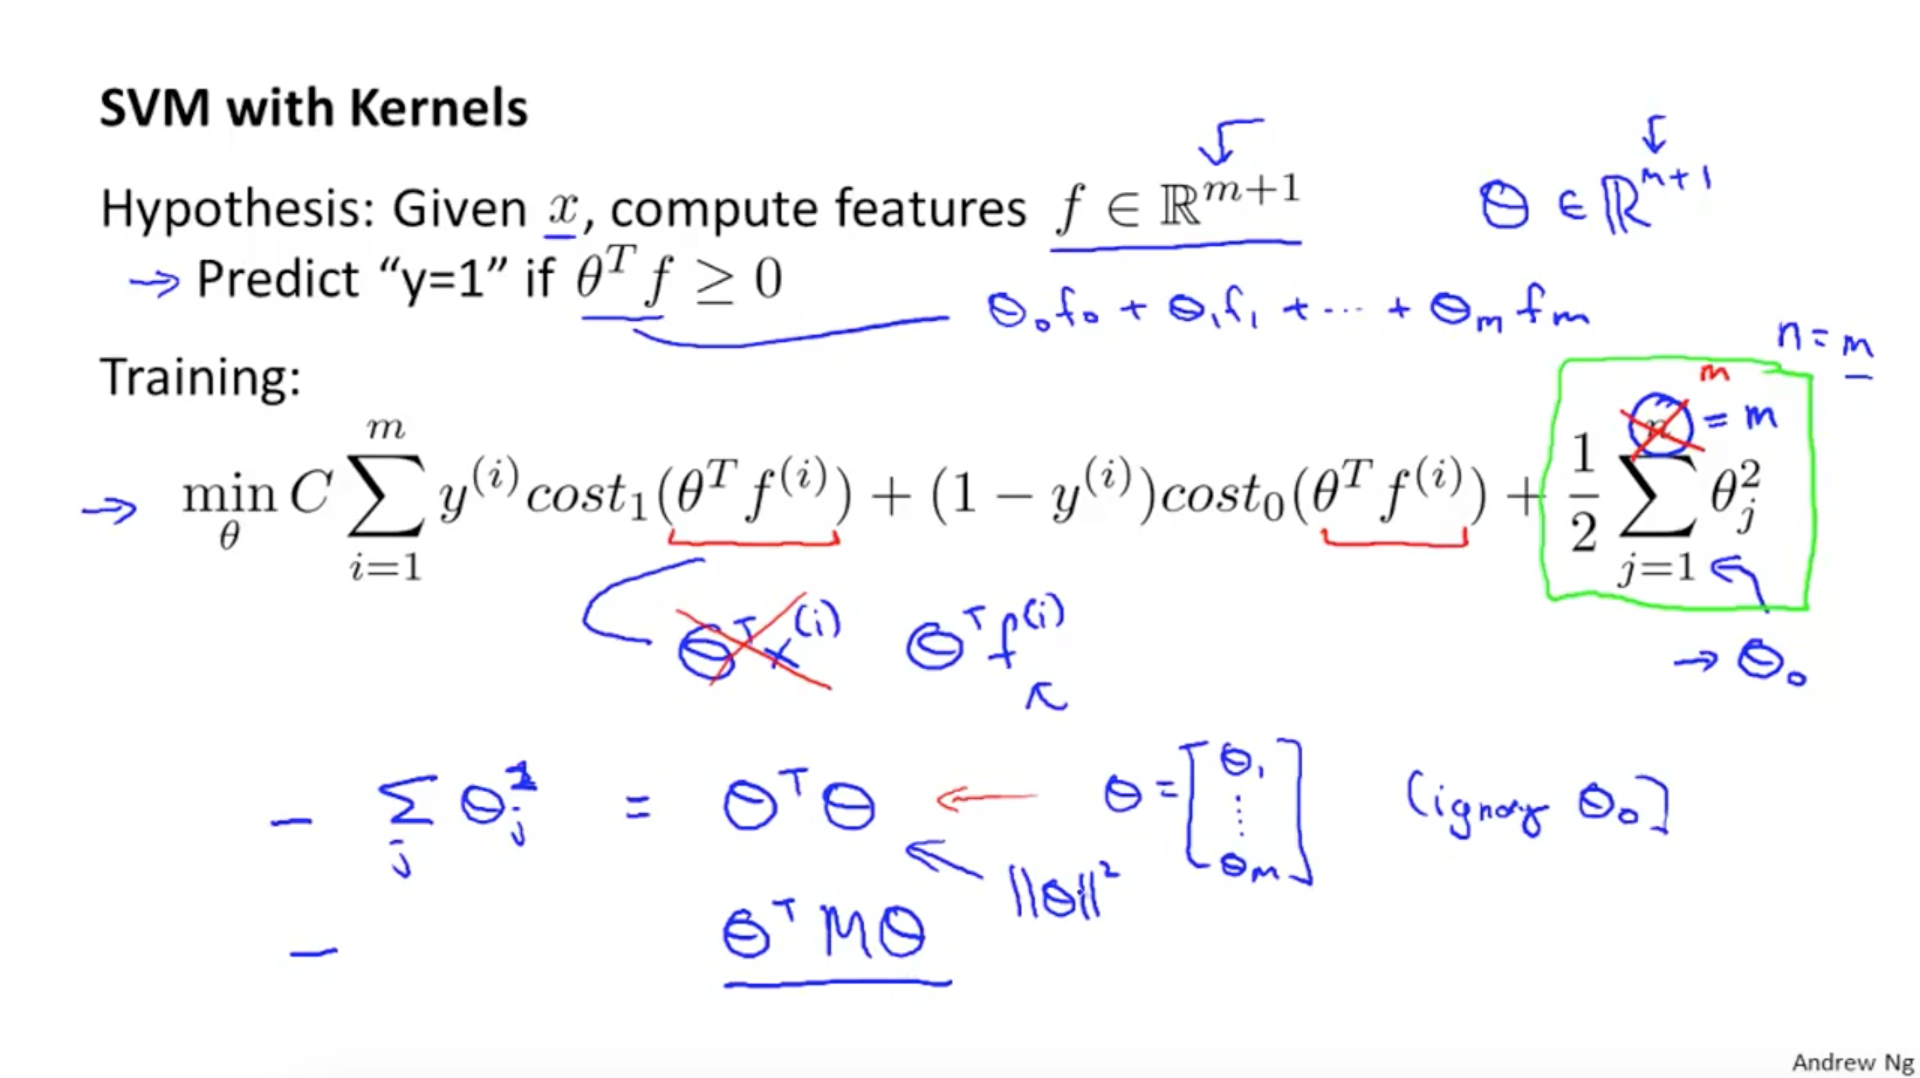
\includegraphics[width= 1.5\textwidth,center]{SVM_Theta_Trick.png}
				\caption{Kernel feature.}
			\end{figure}
			\item Graphic on effects of SVM parameters
			\begin{figure}[ht!]
				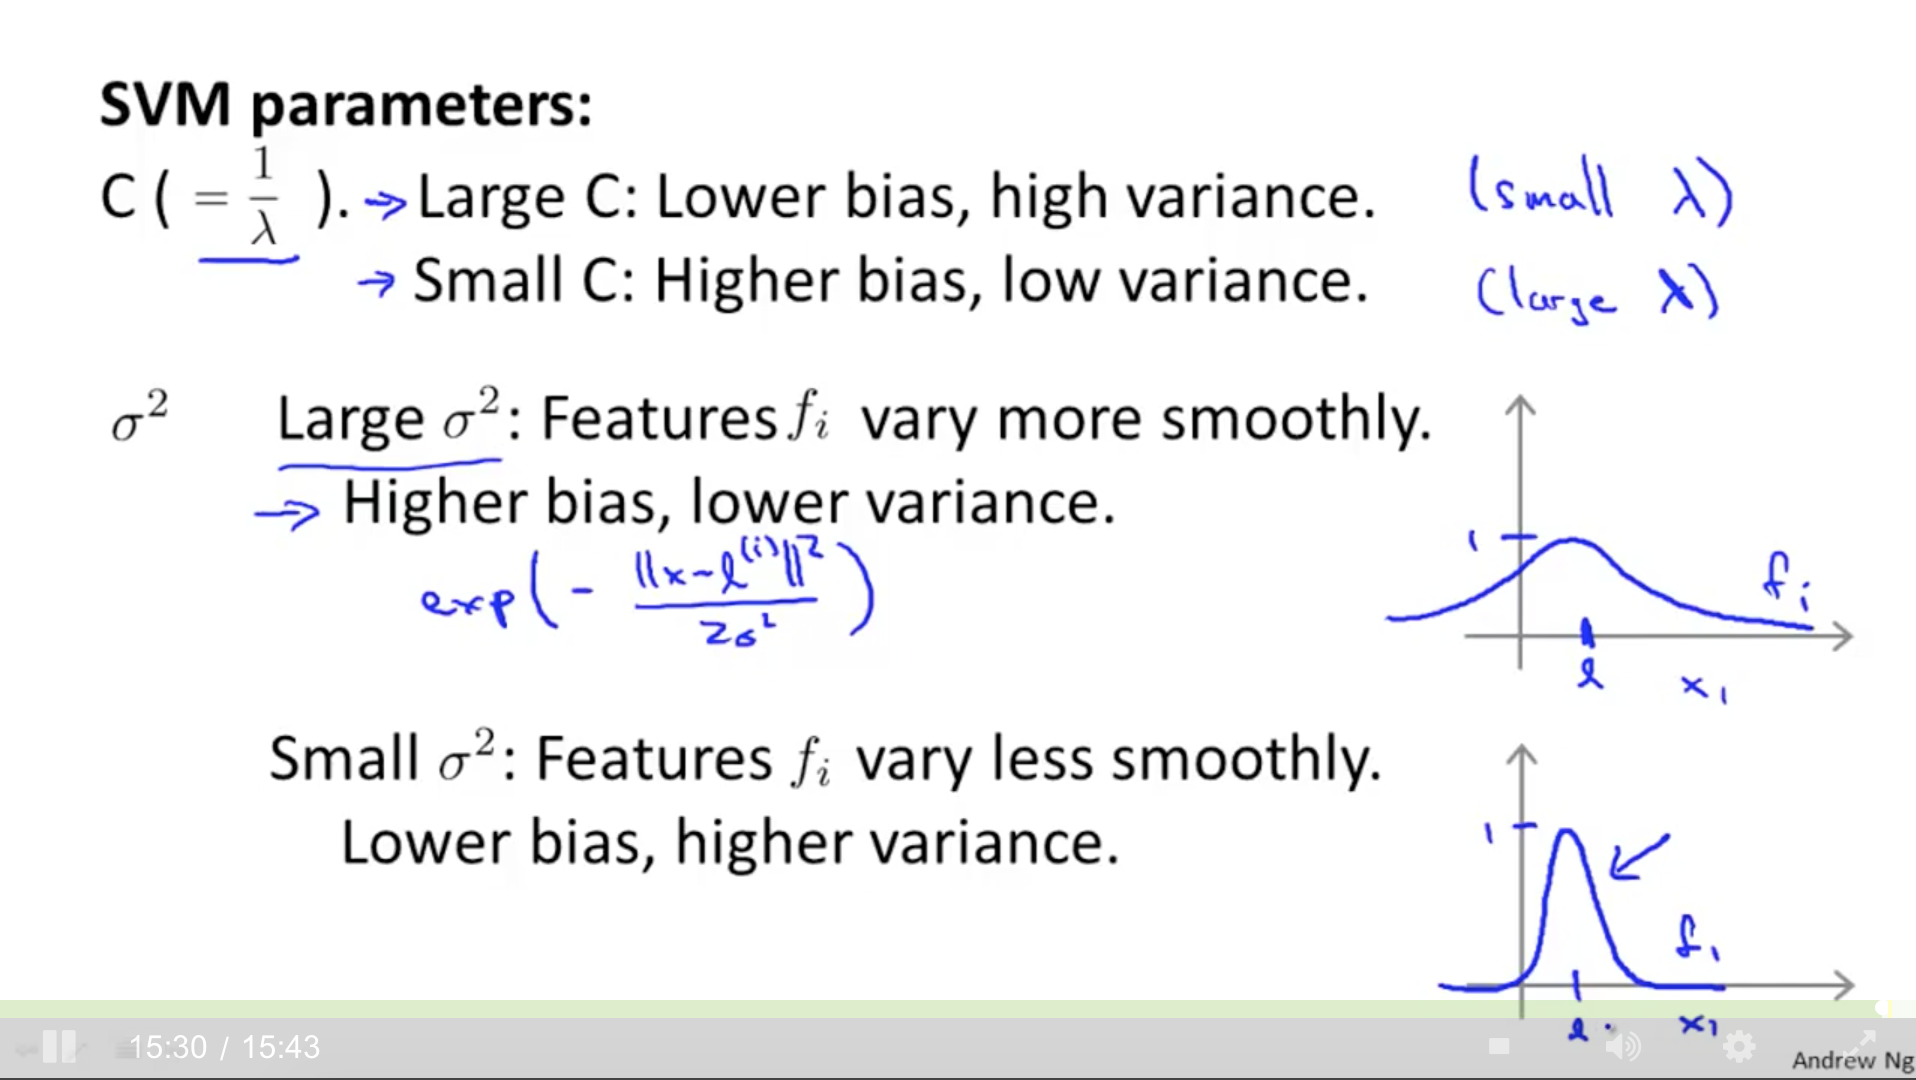
\includegraphics[width= 1.5\textwidth,center]{SVM_parameters.png}
				\caption{Kernel feature.}
			\end{figure}
		\end{itemize}
		
	\subsection{Using a SVM}
		\begin{itemize}
			\item Will need to choose a value for C
			\item choose a kernel (similarity function) (Can even choose no kernel/linear kernel, with $\theta^Tx>=0$
			\item choose a kernel (could be gaussian kernel)
			\item remember to do feature scaling before using the gaussian kernel!
			\item choose $\sigma^2$
			\item \emph{Multi-class classification}
			\item SVM packages generally come with multi-class classification functionality, if not, use one vs. all
			\item if \# of features is large, try logistic regression, or SVM without a kernel
			\item note: SVM - no local minima it could get stuck on compared to neural networks
		\end{itemize}

\section{Unsupervised Learning}
Unsupervised learning is where we have our data set X, but we don't have a y. That is, we have an algorithm find the relation in the data for us.
	\subsection{Clustering: K-means Algorithm}
		\begin{itemize}
			\item This is the most popular clustering algorithm!
			\item (Rough idea of how it works)
			\item We initialize 2 (some number) cluster centroids randomly
			\item We go through each point and try to assign each oint to the 2 cluster centroids
			\item We move the centroids closer to the sets' means.
			\item We repeat the last 2 steps again until we have them all bundled up into groups
			\\
			\item (More accurately, but still in general)
			\item We take input K (number of clusters)
			\item and a training set X
			\item This time, we don't use $x_0=1$
			\item Now randomly init(ialize) the K centroids
			\item Repeat \{
			\item 	for $i$ = 1 to $m$
			\item 		$c^{(i)} :=$ index (from 1 to $K$) of cluster centroid closest to $x^{(i)}$
			\item 	for $k$ = 1 to $K$
			\item 		$\mu_k :=$ average (mean) of points assigned to cluster $k$
			\item \}
			\item The first loop assigns x's to clusters they're closest to (and minimizes J wrt c's, and holds $\mu$'s)
			\item The second gets the mean and moves the centroids to the means (chooses $\mu$'s that minimize J)
			\item If a cluster has no points, we usually remove it. Or, some times we can re-init it.
			\begin{figure}[ht!]
				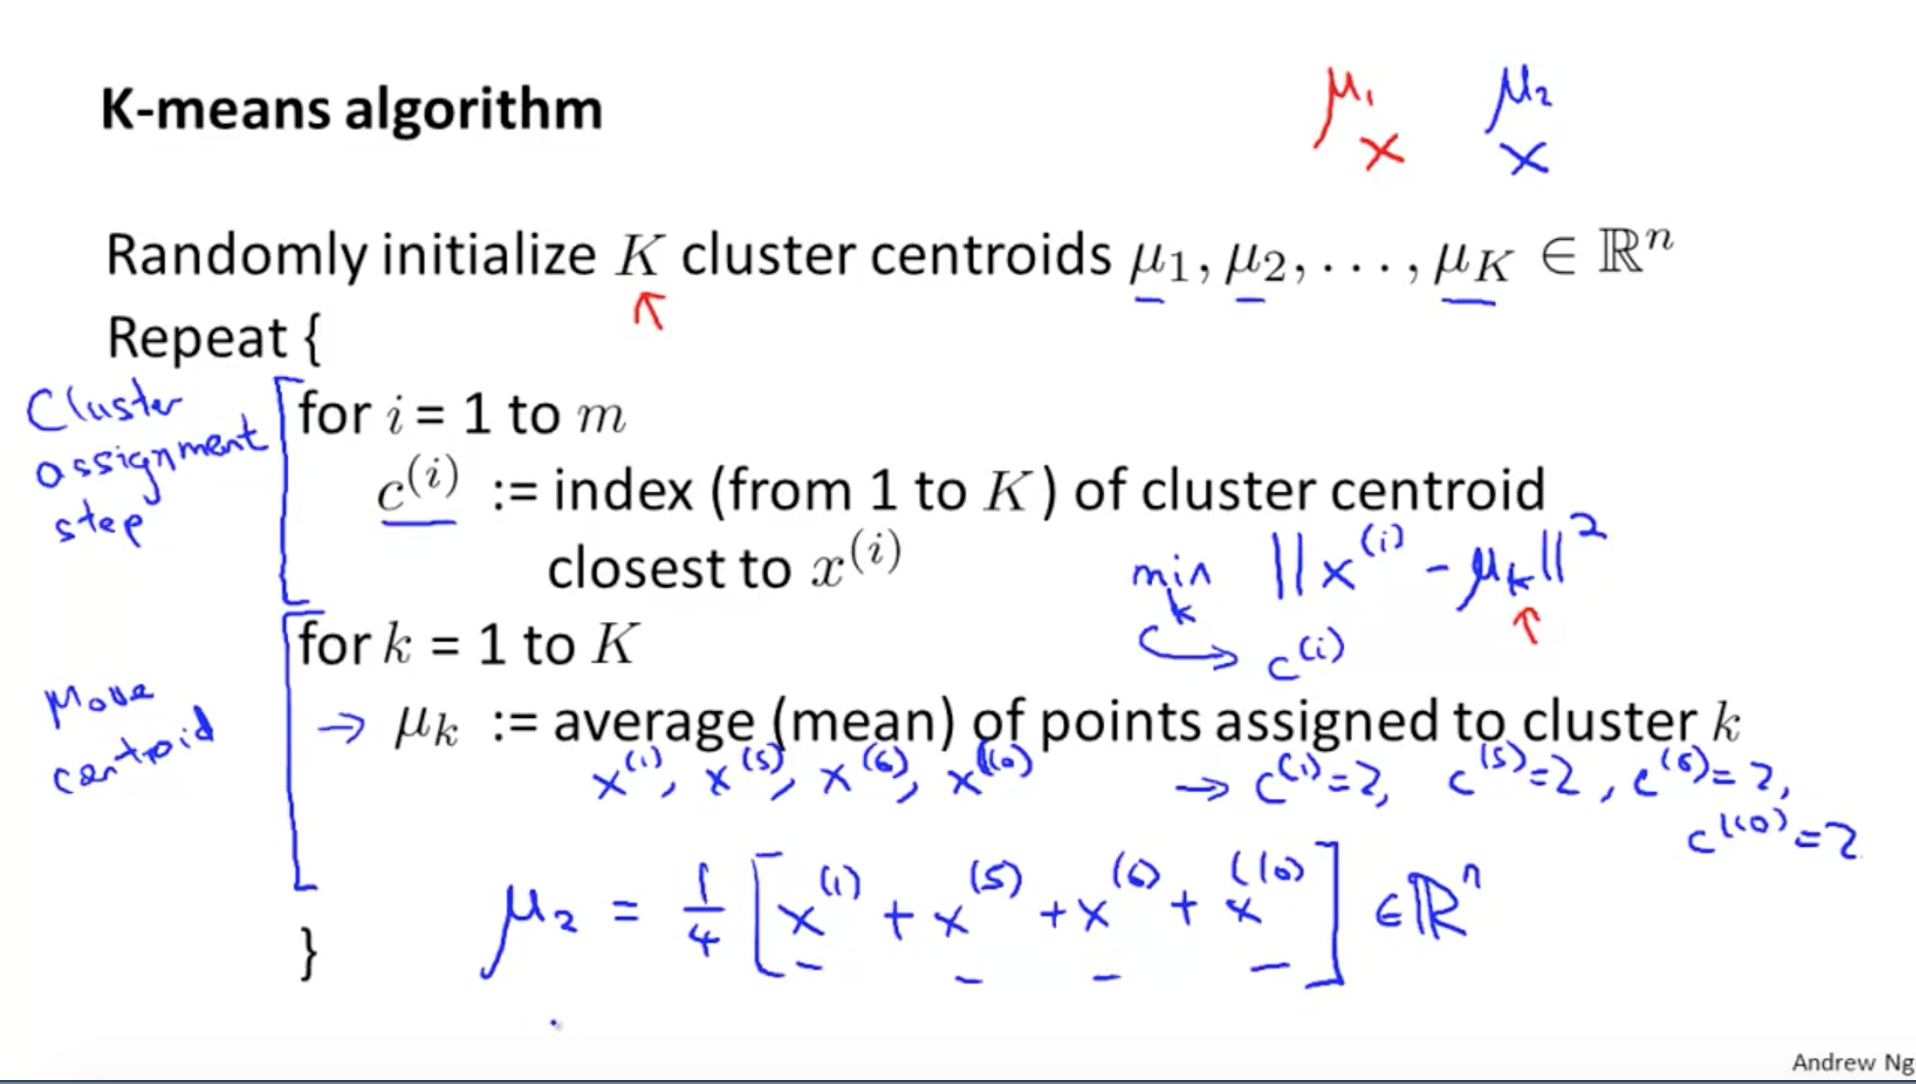
\includegraphics[width= 1.5\textwidth,center]{K-means_Clustering.png}
				\caption{This can also be explained mathematically, but it's out of scope of the course. Maybe I'll add it if I get the chance}
			\end{figure}
			\item K-means for \underline{non-separated clusters}
			\item It will try to make different segments, even if it just looks like a big group a points on graph.
		\end{itemize}
		
	\subsection{Optimization Objective}
		\begin{itemize}
			\item K-means optimization objective
			\item Notation We Will Use:
			\begin{itemize}
				\item $c^{(i)}$ = index of cluster (1 to K) to which $x^{(i)}$ is currently assigned
				\item $\mu_{k}$ = cluster centroid number k
				\item $\mu_{c^{(i)}}$ = cluster centroid of cluster to which $x^{(i)}$ has been assigned
			\end{itemize}
			%\item 
			\begin{figure}[ht!]
				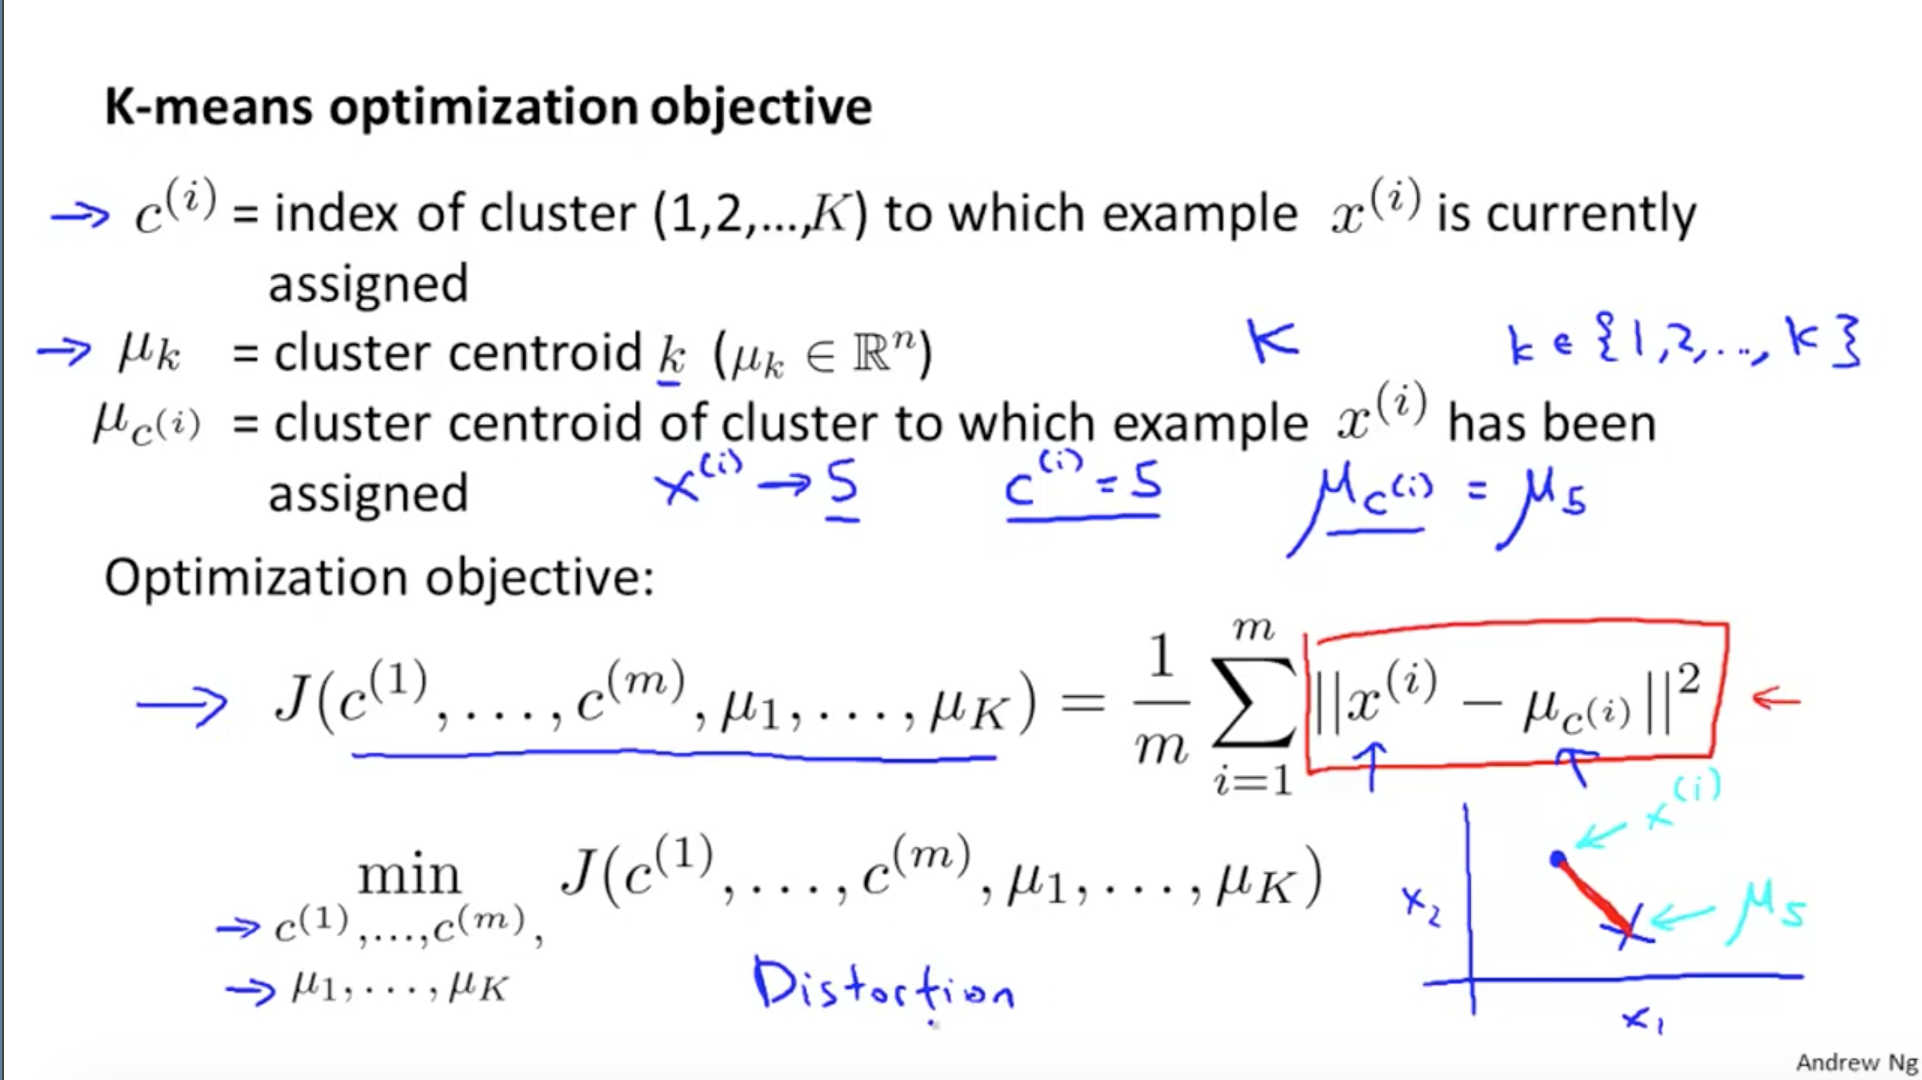
\includegraphics[width= 1.5\textwidth,center]{K-means_Optimization.png}
				\caption{J, the optimization or "distortion" for this clustering algorithm}
			\end{figure}
		\end{itemize}
		
	\subsection{Random Initialization}
		\begin{itemize}
			\item There's actually a good (well, better i should say) way to randomly pick K centroids.
			\item Depending on the init, K-means can end up at different local optima, and not your desired global optima
			\item Solution? We init K-means many times to try to ensure that we reach the global optima
			\item After that, we just pick the one with the lowest J!
			\item We can just use a for loop to do this 50-1000 times (try to see if there's a way to vectorize this code).
			\item But when you have 100's of clusters, this is unlikely to be of much help. The first try might as well be as good as it gets.
		\end{itemize}
		
	\subsection{Choosing the Number of Clusters}
		\begin{itemize}
			\item It might be hard to try to figure out. (could be ambiguous)
			\item Could try the \emph{Elbow Method}
			\item So try and graph the cost Vs. different K's (num of clusters)
			\item Called elbow method since it looks something like a elbow usually
			\item But it's usually not helpful since it usually is a smoother curve and we can't easily find this elbow point that acts as the optimum
			\item So, we could try \emph{Choosing the value of K}
			\item For example, if we have T-shirt sizes based on weight and height, we can try 3 clusters, S, M, L or 5 clusters, XS, S, M, L, XL
		\end{itemize}
		
	\subsection{Dimensionality Reduction}
		\begin{itemize}
			\item \emph{Motivation I: Data Compression}
			\item Ex. 2d to 1d, all the points on the line can be used to represent the 2d data it came from
			\item Ex. 3d to 2d, all the points can be projected to some 2d plane
			\item \emph{Motivation II: Data Visualization}
			\item Hard to visualize many features at once
			\item We can reduce this many dimensional thing into a 2d problem to visualize
		\end{itemize}
		
	\subsection{Principal Component Analysis Problem Formulation}
		\begin{itemize}
			\item In general, reduce n dimensional data to k dimensional data. We find k vectors, (u1, u2... uk) and project the data onto them while also minimizing the projection error
			\item PCA is NOT linear regression
			\item \emph{Data preprocessing}
			\item good to do feature scaling/mean normalization
			\item just like before, if features are on different scales, subtract the mean, and divide by the standard deviation
			\item Now for the algorithm
			\item We compute the "covariance matrix"
			\item $\Sigma = \frac{1}{m}\sum\limits_{i=1}^{n}(x^{(i)})(x^{(i)})^T$ (here, the left sigma is a matrix, and x is nx1, so the result is a n x n)
			\item Compute "eigenvectors" of matrix $\Sigma$:
			\item the Octave command is [U,S,V] = svd(Sigma); (could use the eig() func. but svd is more stable)
			\item the columns of U go up to n
			\item we can take the first k columns of the U matrix (n x k now)
			\item now transpose it (k x n) and multiply by x (n x 1) so now we have vector z
			\item in code, something like: Ureduced = U(:,1:k); and z = Ureduced'*x;
			\\
			\item \emph{Reconstruction from Compressed Representation}
			\item To get x back, we can multiply this Ureduced matrix (n x k) by the z vector (k x 1), so we get a n x 1 vector back
			\item Of course this x will be approximately close to the original
		\end{itemize}
		
	\subsection{Choosing the Number of Principal Components}
		\begin{itemize}
			\item get average square projection error divided by the total variation less than 0.01
			\item so that "99\% of variance is retained"
			\item We can also use 95-90\% to get more compression
			\item Now to choose k try PCA with k = 1 .... some number
			\item compute U, z etc.
			\item now check the variance
			\item As you can imagine, this is horribly inefficient
			\item So the other way is, looking at octave's [U,S,V] = svd(Sigma), to sum k of S's diagonal elements, divide by the sum of n (all of S's) elements, and subtract this from 1, and see if this is greater or equal to 0.99
			\item After this, we can also check the variance retained by running the calculations with k incase anyone asks what it was (to check)
			\begin{figure}[ht!]
				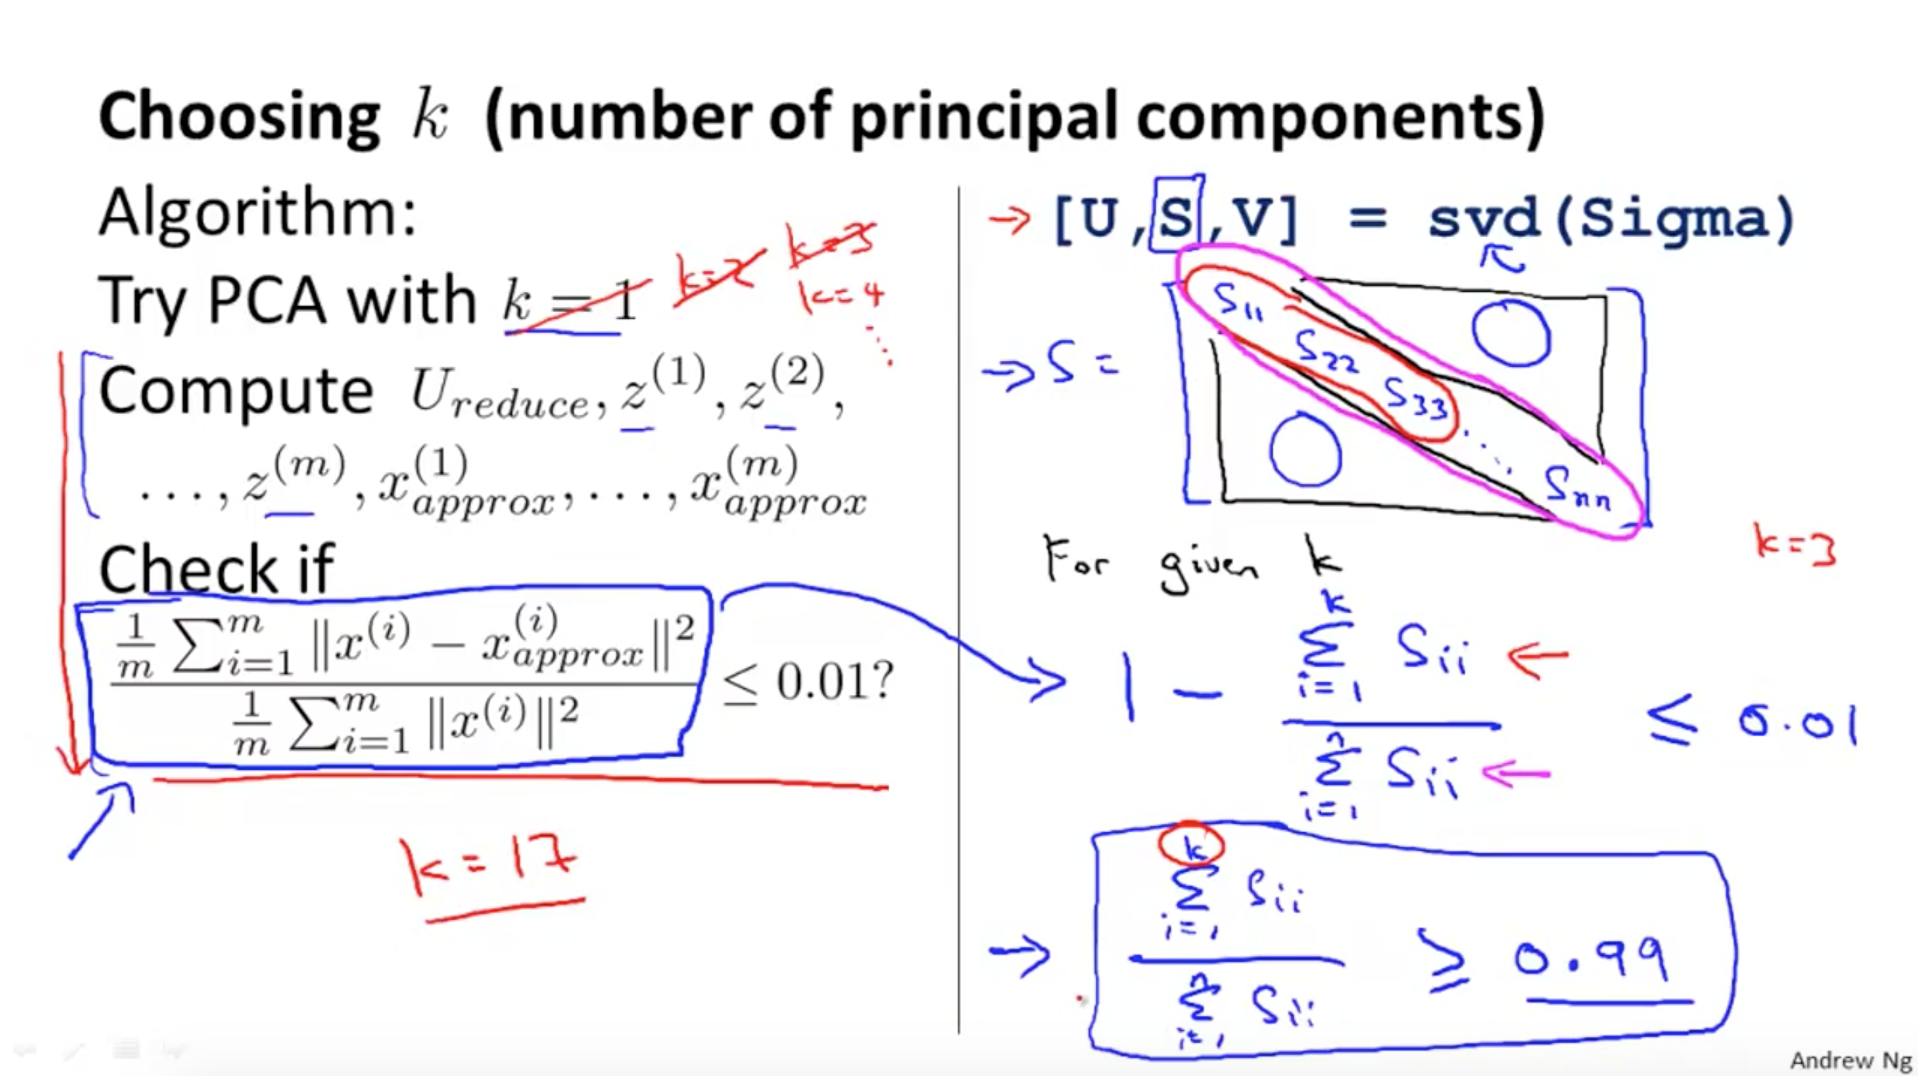
\includegraphics[width= 1.5\textwidth,center]{Choosing_K_PCA.png}
				\caption{To the right, is a good way to check what's a good k without too much work (If you work iwth matlab/octave)}
			\end{figure}
		\end{itemize}
		
	\subsection{Advice for Applying PCA}
		\begin{itemize}
			\item \emph{supervised learning speedup}
			\item We can reduce the dimensions of the data with PCA (let's ignore the y's first)
			\item let's say we took 10,000 feature training examples and made them into 1000 feature examples
			\item now let's match the y's back to these compressed z examples
			\item Note: this mapping of x->z should only be defined with PCA on the training set
			\item now use this mapping for the cross validation set and test set
			\\
			\item Recap: Compression
			\item reduce memory/disk needed to store data
			\item speeds up learning algorithm
			\item OR for visualization (where k = 2 or 3)
			\\
			\item A \emph{BAD USE OF PCA}: to prevent overfitting
			\item This won't really work (well... it might in some odd cases) but it won't in general
			\item Just use regularization
			\\
			\item Note: before just throwing in PCA for ML, try your implementation first without PCA, and then see if you need PCA or not.
			\item Recap: compress data, visualize, and make training data smaller
		\end{itemize}
		
\section{Anomaly Detection}
	\subsection{Problem Motivation}
		\begin{itemize}
			\item Density Estimation is one technique
			\item An application is Fraud Detection
			\item Quick review of Gaussian Distribution
			\begin{figure}[ht!]
				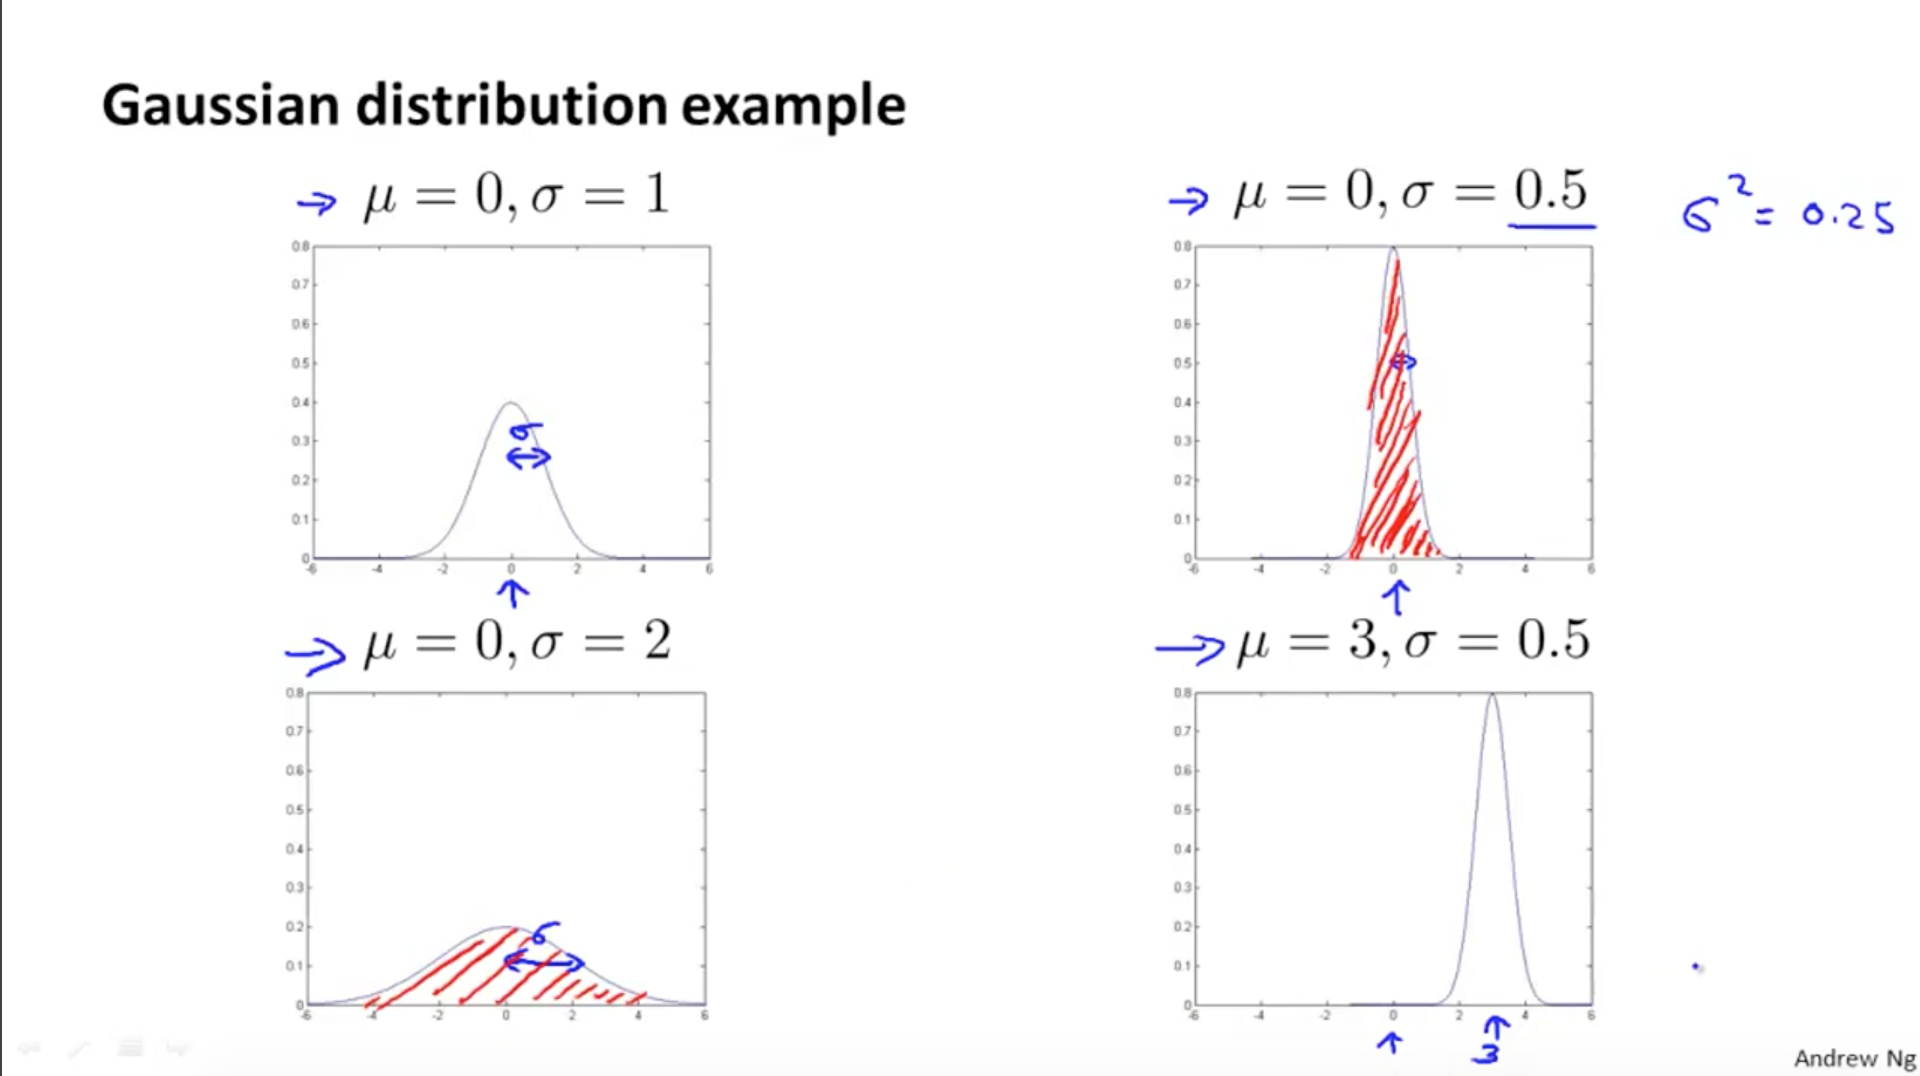
\includegraphics[width= 1.5\textwidth,center]{Gaussian_Review.png}
				\caption{Quick Review on Gaussian Distribution. Note: the area always integrates to 1.}
			\end{figure}
			\item \emph{Parameter Estimation}
			\item Try to guess where the parameters of $\mu$ and $\sigma^2$ (and tell if it's far away from the mean on the gaussian distribution)
			\item So remember Data Management in high school, calculate mu and sigma
			\item $\mu = \frac{1}{m} \sum\limits_{i=1}^{m} x^{(i)}$
			\item $\sigma^2 = \frac{1}{m}\sum\limits_{i=1}^{m} (x^{(i)}-\mu)^2$
			\item Remember that in stats, that sometimes m-1 is used (I already forgot why (normalization i think)) but when m is very large, it doesn't matter if you subtract 1
		\end{itemize}
		
	\subsection{Algorithm}
		\begin{itemize}
			\item \emph{Density Estimation}
			\item we have the training set x1, 2, 3... etc. and each example is $x \in \mathbb(R)^{n}$
			\item So, $x_{i} ~ \mathcal{N}(\mu_i,\sigma_i^2)$, with i being the training examples
			\item and now p(x)
			\item $= p(x_1;\mu_1,\sigma_1^2)p(x_2;\mu_2,\sigma_2^2)...p(x_n;\mu_n,\sigma_n^2)$
			\item OR $\prod\limits_{j=1}^{n}p(x_j;\mu_j,\sigma_j^2)$
			\item Now with this, we can make the algorithm:
			\begin{enumerate}
				\item Choose features $x_i$ that you think might be indicative of anomalous examples
				\item Fit parameters $\mu_1,...,\mu_n,\sigma_1^2,...,\sigma_n^2$, in otherwords, use the equations for mu and sigma
				\item Given new example x, compute p(x)
				\\	$p(x) = \prod\limits_{j=1}^{n}p(x_j;\mu_j,\sigma_j^2) = \prod\limits_{j=1}^{n}\frac{1}{sqrt{2\pi}\sigma_j}exp(-\frac{(x_j-\mu_j)^2}{2\sigma_j^2})$
				\\ Add your condition: Anomaly if p(x) < $\epsilon$
			\end{enumerate}
		\end{itemize}
		
	\subsection{Building an Anomaly Detection System}
		\begin{itemize}
			\item train the program with mostly non-anomalous data
			\item include a few examples in the x-validation and test set
			\item Note: as mentioned before, good evaluation metrics are use the true positives and stuff, precisions/recall, and F-score.
			\item Can also can use validation set to pick a good $\epsilon$
		\end{itemize}
		
	\subsection{Anomaly Detection vs. Supervised Learning}
		\begin{itemize}
			\item Anomaly detection: Use if -
			\item - small \# of positive examples (y=1) (0-20 is a common amount)
			\item - large \# of negative examples (y=0)
			\item - Many diff "types" of anomalies. Hard for an algorithm to learn from positive examples what anomalies look like, so easier to just learn what negative examples look like and just flag things that are different
			\item -future examples may not look like the examples we have trained on
			\item Ex. - Fraud detection (easier if only a few occurrences of fraud in your company)
			\item Ex. -  Manufacturing (again, easier if only a few occurrences, otherwise be better to use Supervised Learning)
			\item Ex. - Monitoring machines in data center (again, same argument)
			\item Supervised Learning: Use if -
			\item - large \# of positive and negative examples
			\item - we have enough positive examples and are confident future positive examples will be similar
			\item Ex. - Spam Classification
			\item Ex. - Weather prediction
			\item Ex. - Cancer Classification
		\end{itemize}
		
	\subsection{Choosing What Features to Use}
		\begin{itemize}
			\item Note: This is mainly about choosing features with values that will act out when an anomaly occurs
			\item Note: first, try to plot a histogram (hist function in Matlab/Octave) to see it it looks gausian (it's ok if it doesn't look gaussian, it'll probably still work)
			\item That, or try taking the log, square root, cube root, etc. of the histogram to see if that makes it look gaussian
			\item Note: the histogram command is something like hist(x) or hist(x, numOfBins) And the run it on a vector or matrix x
			\\
			\item Picking features
			\item try some Error analysis for anomaly detection
			\item want p(x) large for normal examples of x and small for anomalous examples. (to fit the gaussian curve)
			\item Common Problem: p(x) is large comparable (similar magnitude) for normal and anomalous examples
			\item So try to find a feature that would give better information.
			\\
			\item Examples: Monitoring computers in a data center
			\item choose features that might take unusually large or small values in the event of an anomaly
			\item let's say we have:
			\item x1 = memory use of computer 
			\item x2 = number of disk accesses/sec
			\item x3 = CPU load
			\item x4 = network traffic
			\item this is good, but we might get more info from connecting some info together, like x5 = $\frac{CPU load}{network traffic}$ or x6 = $\frac{(CPU load)^2}{network traffic}$
		\end{itemize}
		
	\subsection{Multivariate Gaussian Distribution}
		\begin{itemize}
			\item Sometimes you might have 2 features that each score 0.2, but it isn't high enough to be flagged as an anomaly, but it would be if it were on a 3D plot
			\begin{figure}[ht!]
				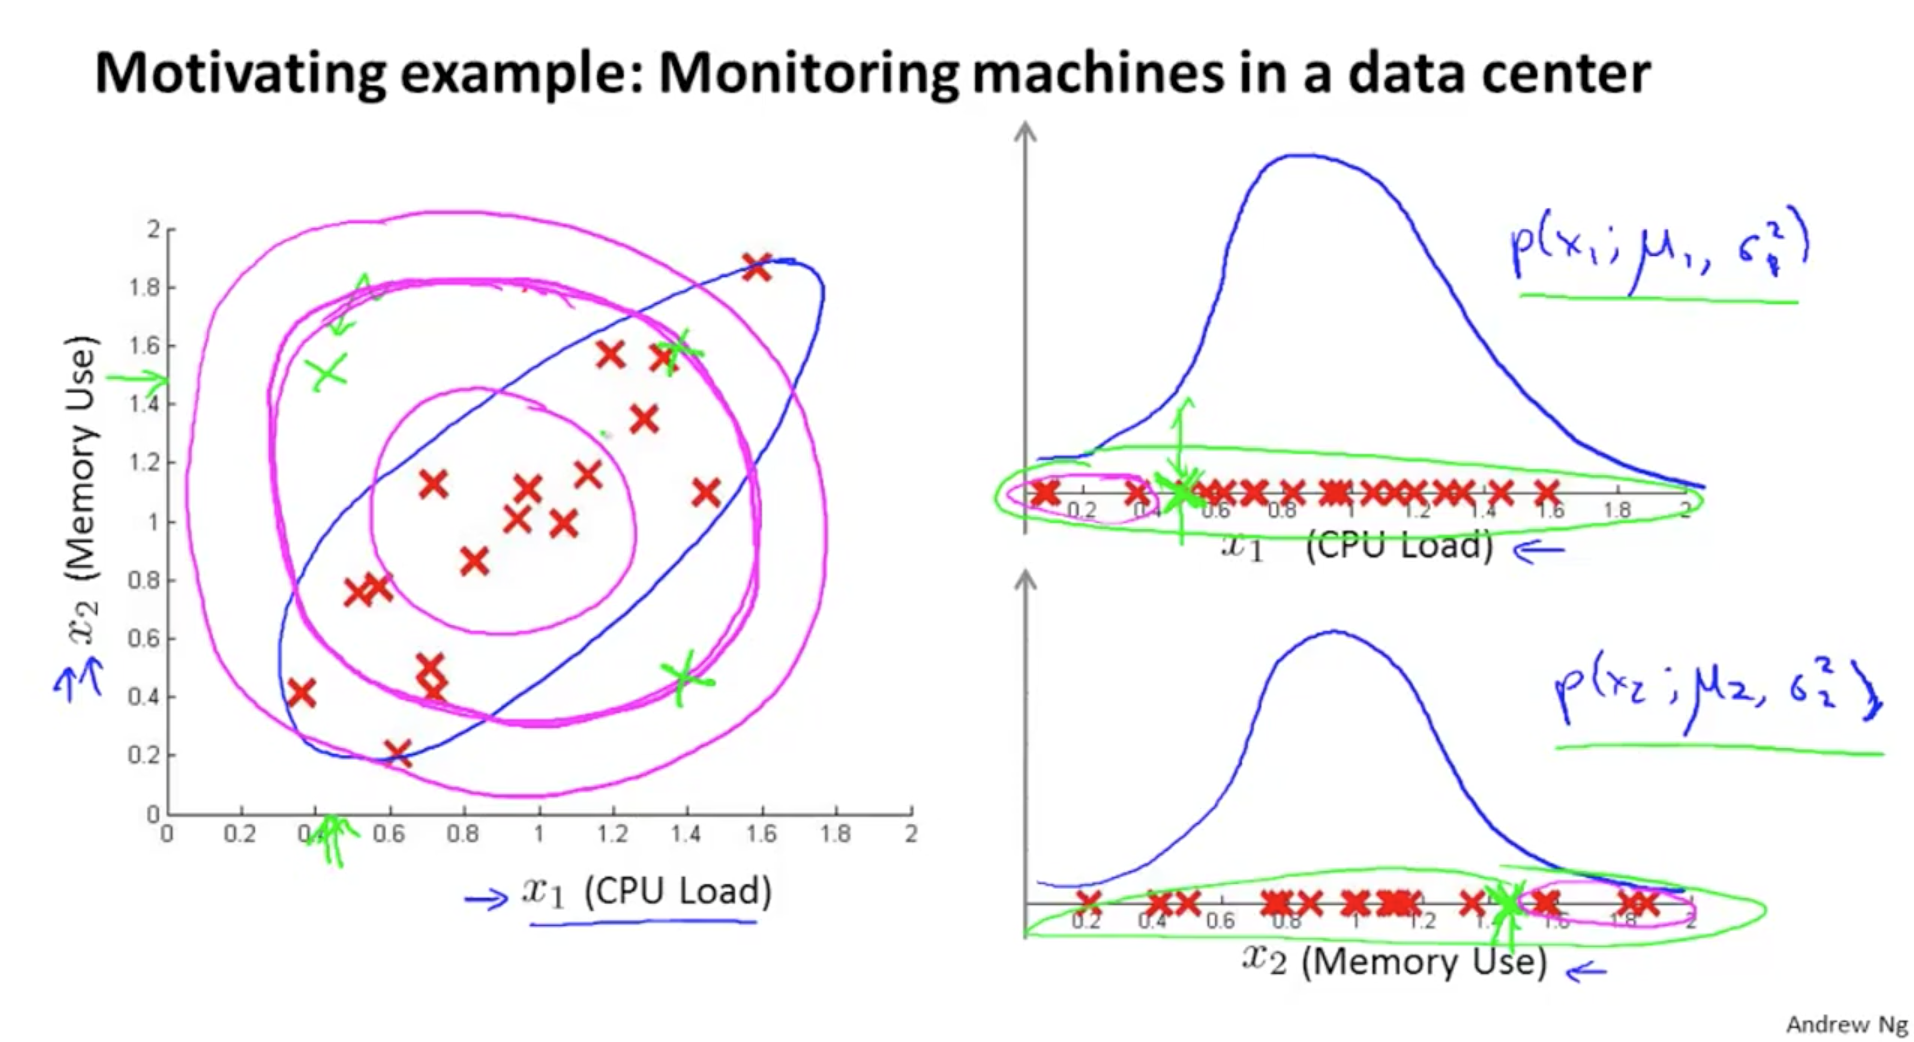
\includegraphics[width= 1.5\textwidth,center]{Multivariate_Gaussian.png}
				\caption{When we move to a 3D plot, it's clear that the 2 green points are anomalies}
			\end{figure}
			\item \emph{Multivariate Gaussian (Normal) Distribution}
			\item $x \in \mathbb{R}^n$ don't model $p(x_1),p(x_2)$... etc. separately
			\item model them altogether
			\item Parameters: $\mu \in \mathbb{R}^n,\Sigma \in \mathbb{R}^{n x n}$ (covariance matrix)
		\end{itemize}
		
	\subsection{Anomaly Detection using the Multivariate Gaussian Distribution}
		\begin{itemize}
			\item remember, we have parameters $\mu \in \mathbb{R}^n,\Sigma \in \mathbb{R}^{n x n}$
			\item But to get this p we use:
			\item $p(x;\mu,\Sigma)=\frac{1}{(2\pi)^{\frac{n}{2}}|\Sigma|^{\frac{1}{2}}}exp(1\frac{1}{2}(x-\mu)^T\Sigma^{-1}(x-\mu))$
			\item and to get $\mu$ and $\Sigma$
			\item $\mu = \frac{1}{m} \sum\limits_{i=1}^{m} x^{(i)}$
			\item $\sigma^2 = \frac{1}{m}\sum\limits_{i=1}^{m} (x^{(i)}-\mu)(x^{(i)}-\mu)^T$
			\begin{enumerate}
				\item fit model p(x) by setting $\mu$ and $\Sigma$
				\item given new example x, compute p(x), and flag as anomaly if p(x) < $\epsilon$
			\end{enumerate}
			\item turns out our old not multivariate model is a variation of the multivariate Gaussian, just with the $\Sigma$ with zeros everywhere except the diagonal
			\item \emph{Original model vs. Multivariate Gaussian}
			\item Original Model:
			\item might need to manually create features to spot anomalies (like that thing with the cpu load and memory use)
			\item computationally cheaper, also scales better to large $n$ (could be 100's of 1000's)
			\item it works even if $m$ (training set size) is small
			\item Multivariate Model:
			\item automatically capture correlations between features
			\item but computationally more expensive
			\item must have $m > n$, or else $\Sigma$ is non-invertable
			\item better to use only if m is much greater than n (maybe 10 times n)
			\item also won't work if there are redundant features, like duplicated features
			\item (in other words, linearly dependent features aren't good)
		\end{itemize}
		
	\subsection{Problem Formulation}
		\begin{itemize}
			\item VERY USEFUL FOR COMPANIES LIKE AMAZON, NETFLIX, etc. (can recommend products to consumers to make lots of \$\$\$)
			\item Some notation we'll use for now is:
			\item $n_u$ = no. users
			\item $n_m$ = no. movies
			\item $r(i,j)$ = 1 if user $j$ has rated movie $i$
			\item $y^{(i,j)}$ = rating given by user $j$ to movie $i$ (defined only if $r(i,j)$ = 1)
			\begin{figure}[ht!]
				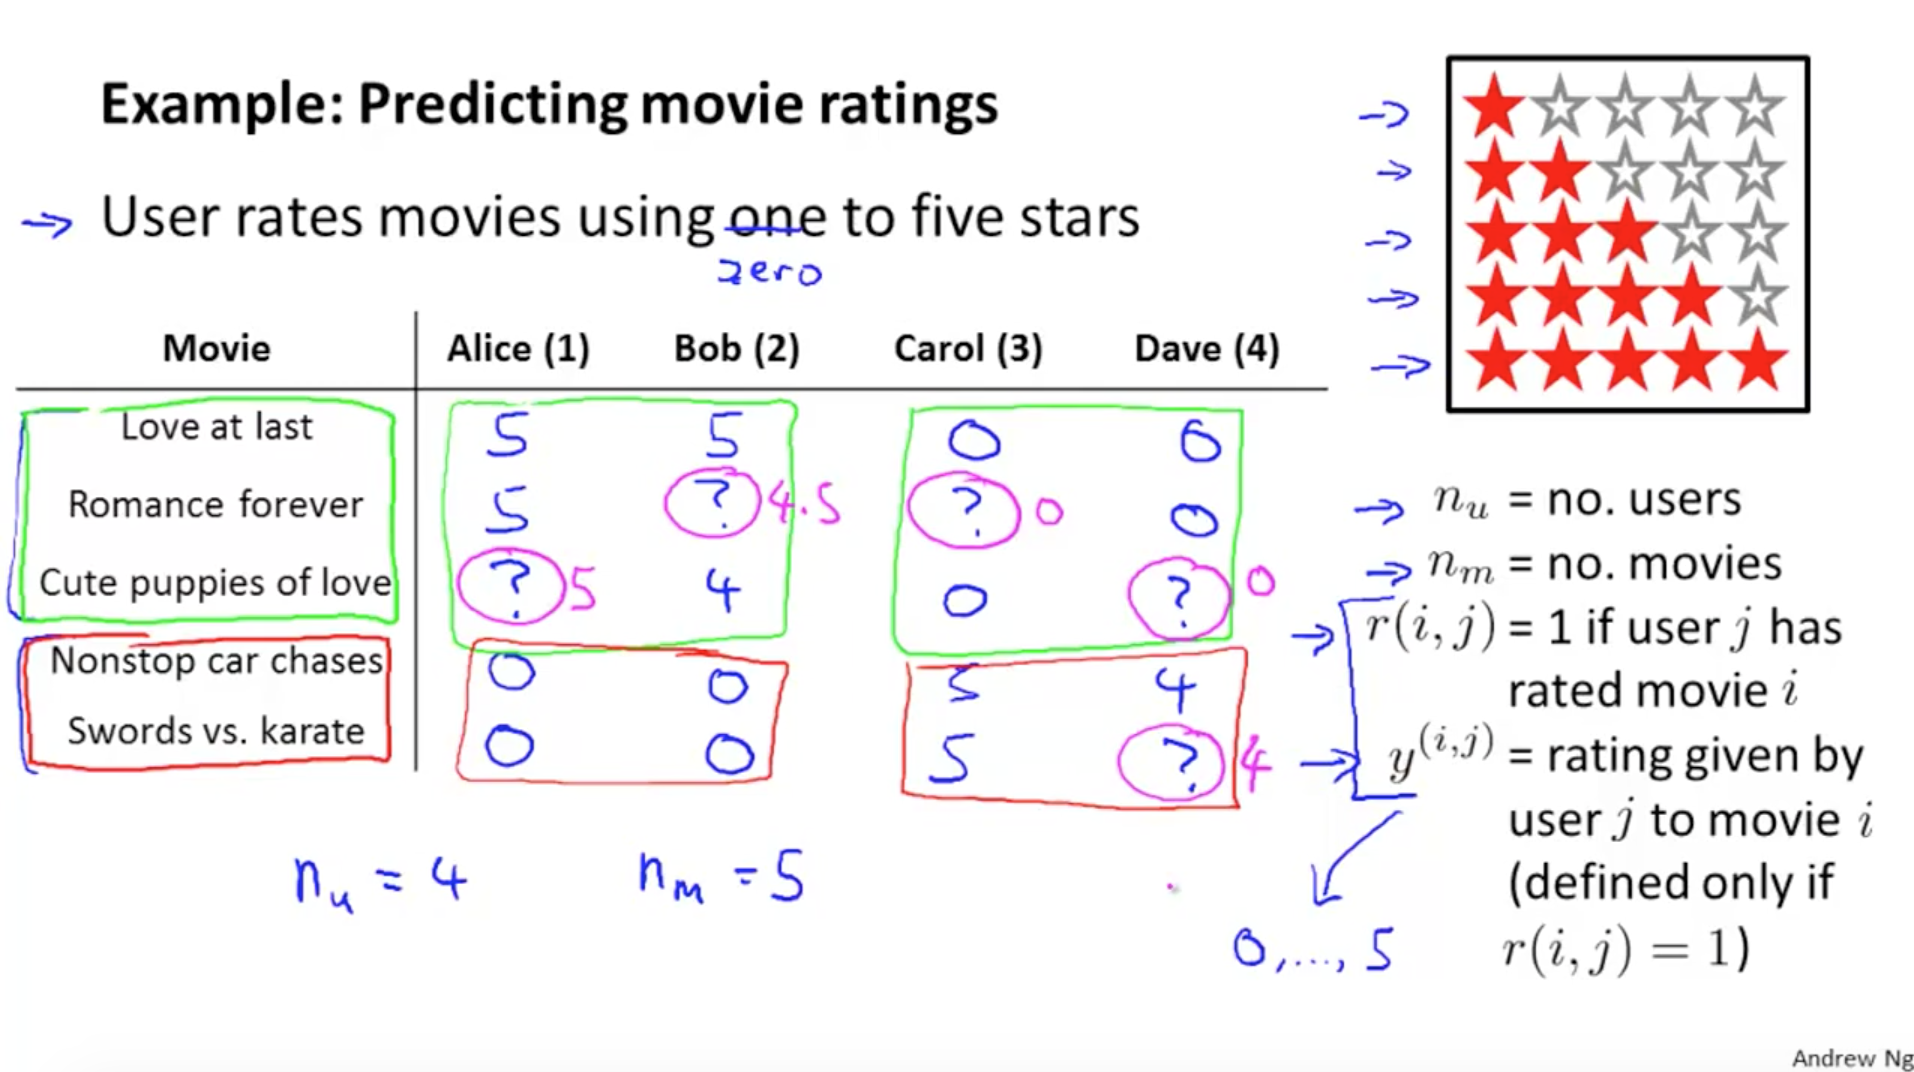
\includegraphics[width= 1.5\textwidth,center]{Movie_Ratings_Example.png}
				\caption{An example}
			\end{figure}
		\end{itemize}
		
	\subsection{Content Based Recommendations}
		\begin{itemize}
			\item Let's say we had ratings for the genres of each movie, (like a movie had a rating for romance, and action), we would then have a feature vector
			\item the rest becomes linear regression
			\begin{figure}[ht!]
				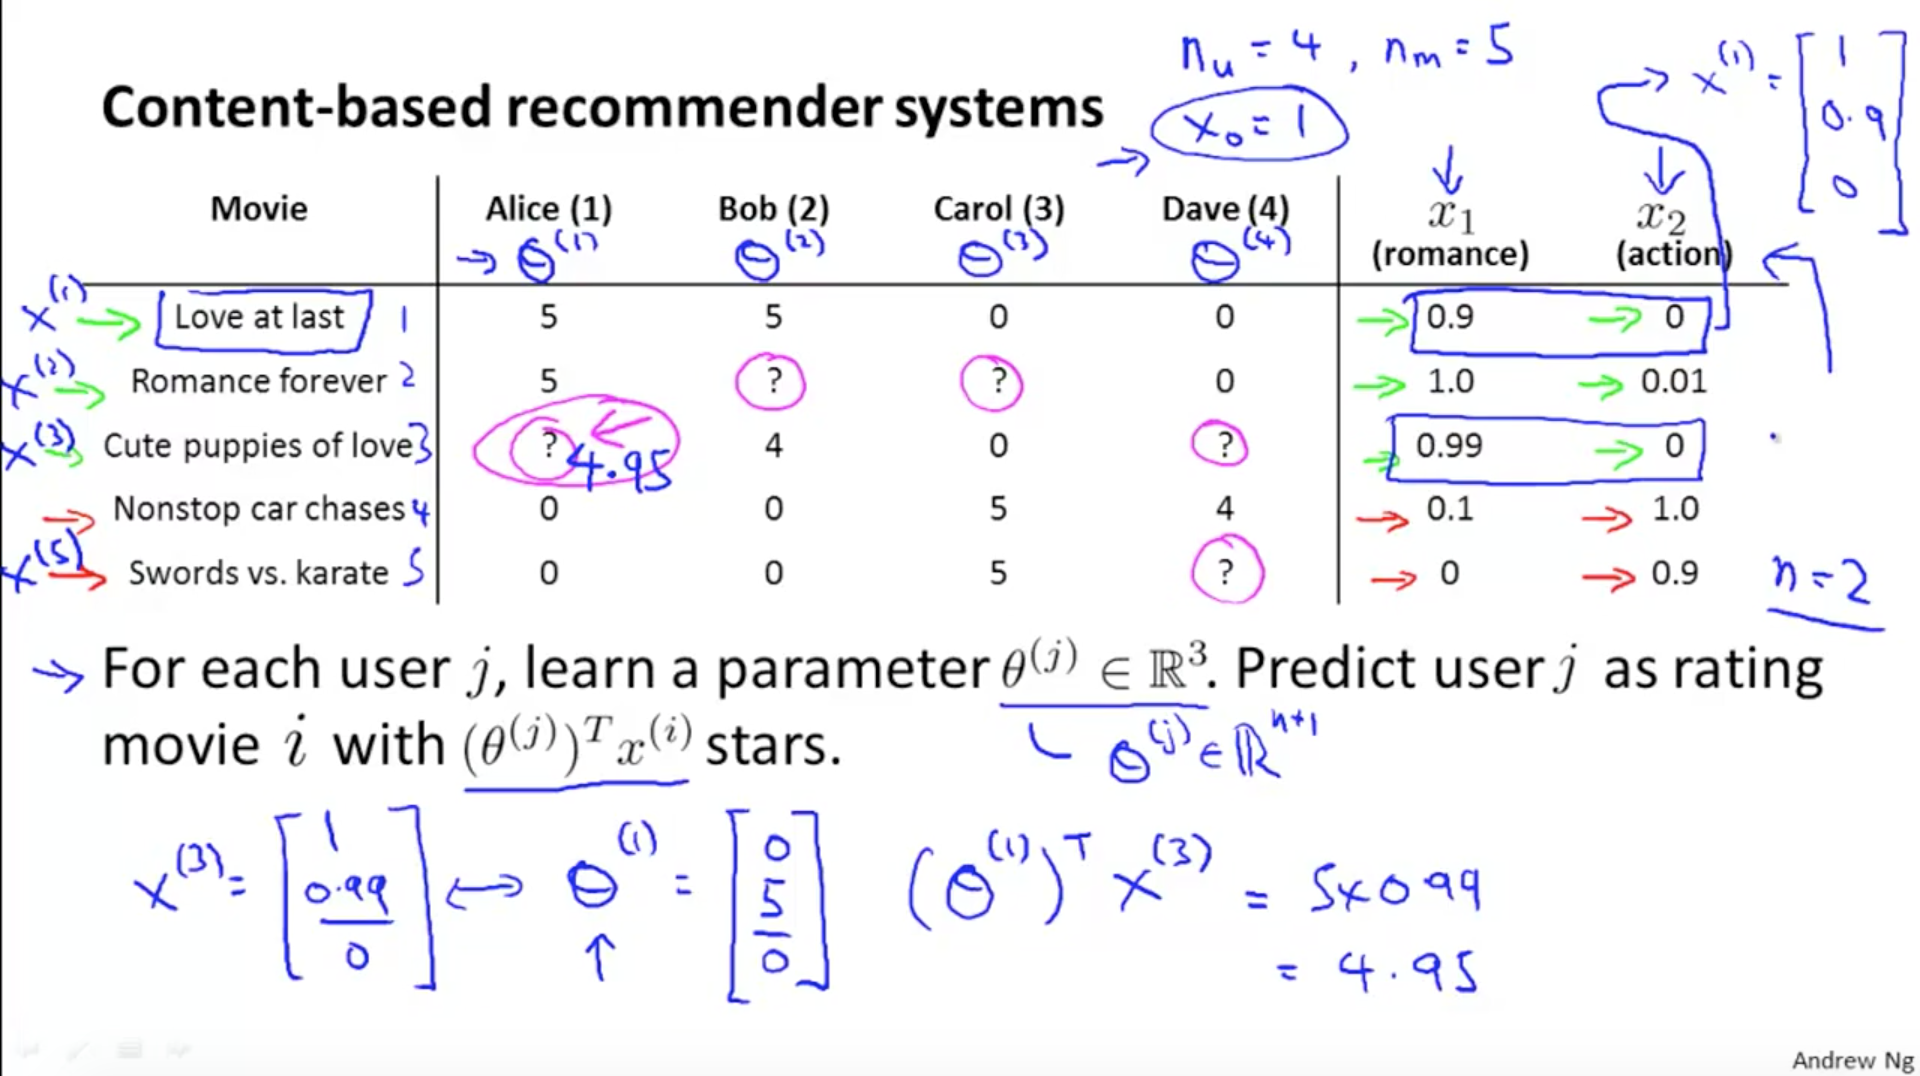
\includegraphics[width= 1.5\textwidth,center]{Content_Example.png}
				\caption{How to predict ratings}
			\end{figure}
			\begin{figure}[ht!]
				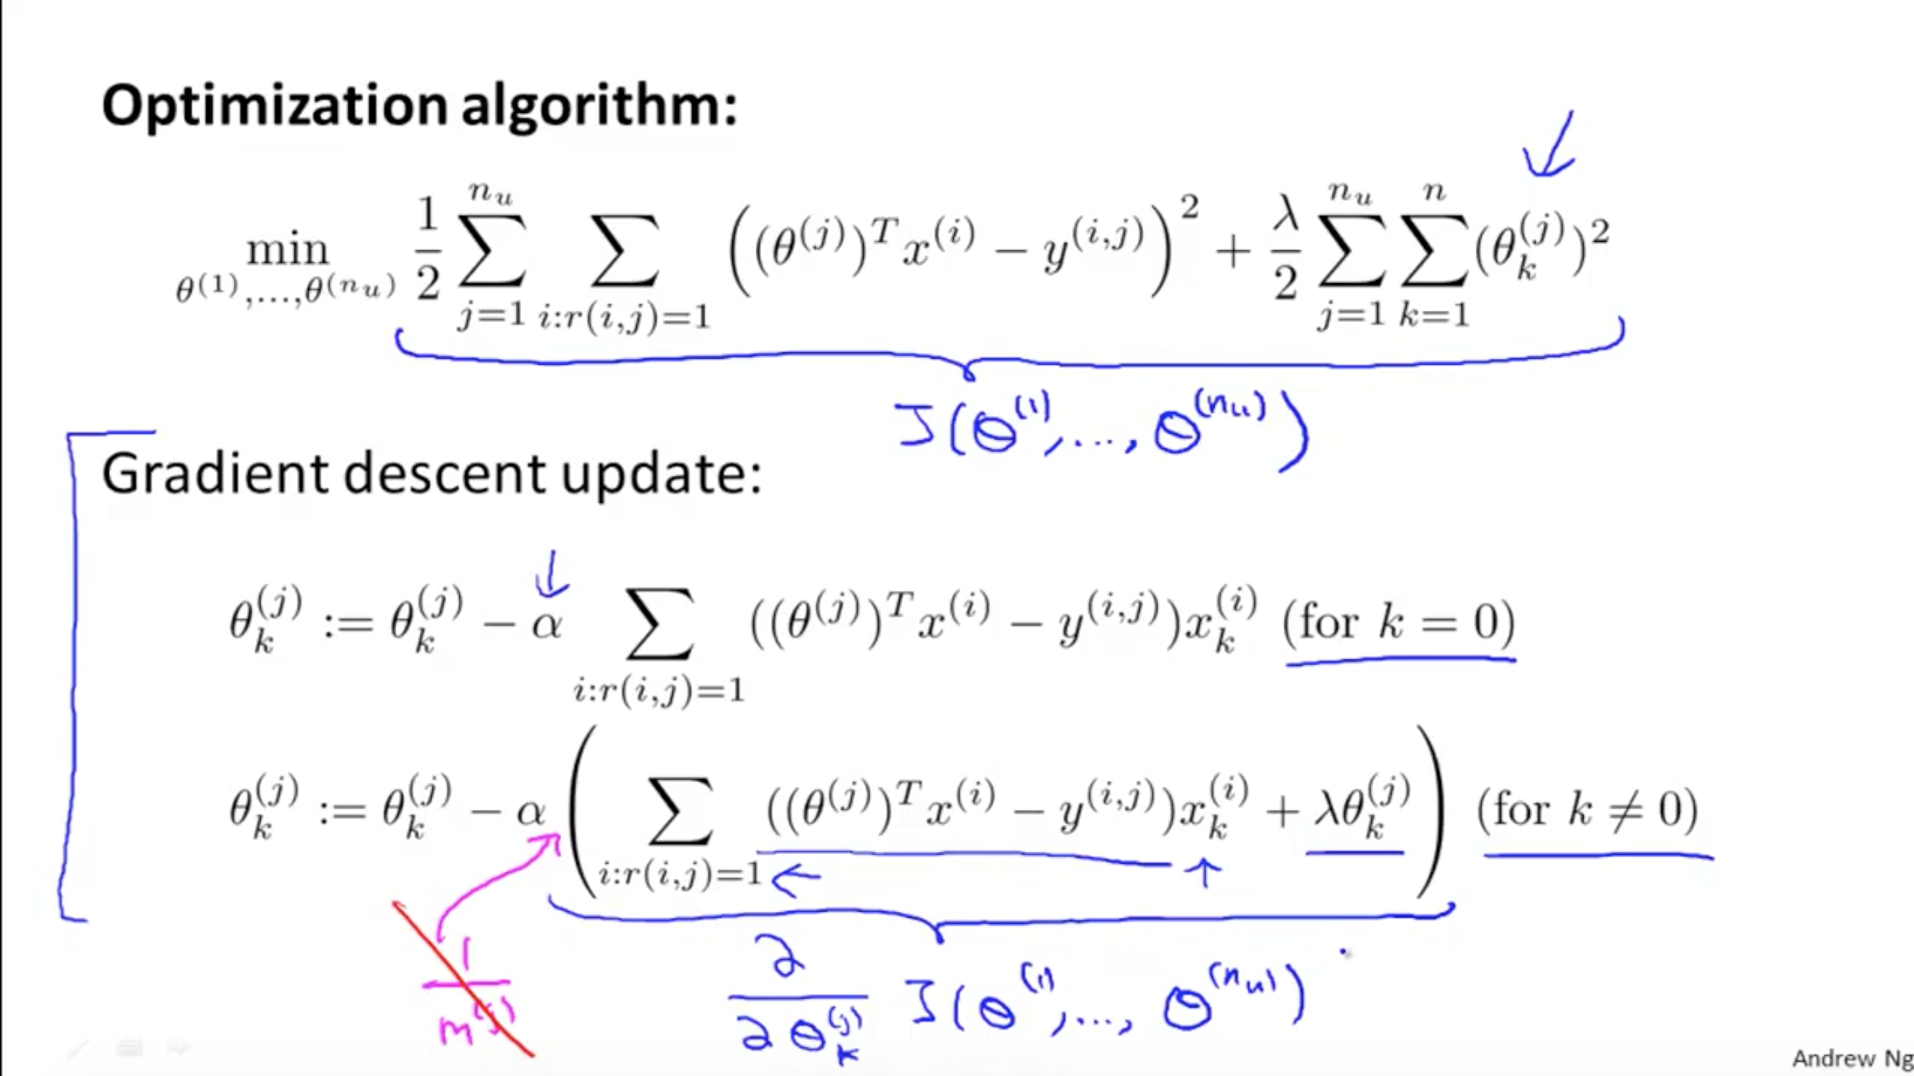
\includegraphics[width= 1.5\textwidth,center]{Optimization_For_Recommender.png}
				\caption{How to optimize the fn. Remeber, it's possbile to also use an implementation of a more complex algoirthm than gradient descent.}
			\end{figure}
		\end{itemize}
		
	\subsection{Collaborative Filtering}
		\begin{itemize}
			\item (Initialize thetas to random values, just like in neural networks) guess a theta term first, the minimize theta, then x, then theta, then x, etc.
		\end{itemize}
		
	\subsection{Collaborative Filtering Algorithm}
		\begin{itemize}
			\item I'll be lazy for this part and just include some snapshots
			\begin{figure}[ht!]
				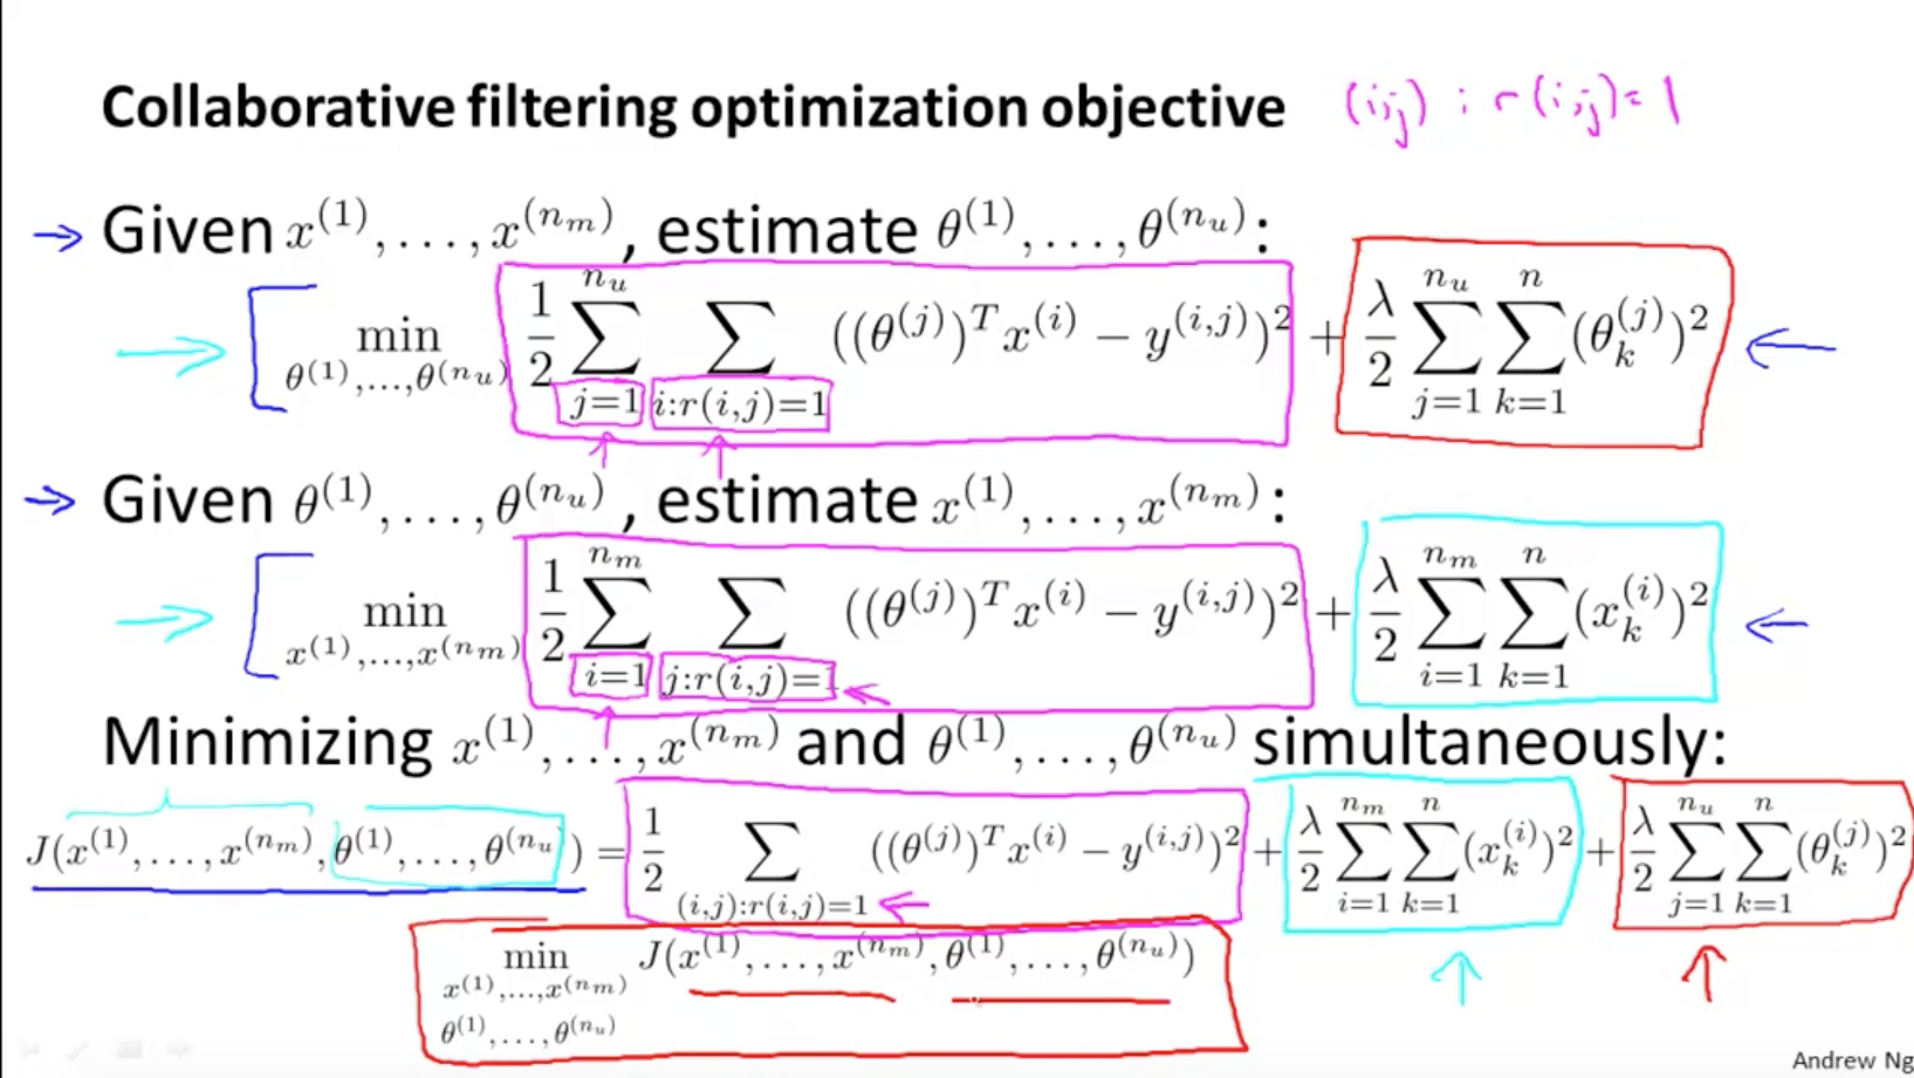
\includegraphics[width= 1.5\textwidth,center]{Collaborative_Filtering_Objective.png}
				\caption{What to optimize}
			\end{figure}
			\begin{figure}[ht!]
				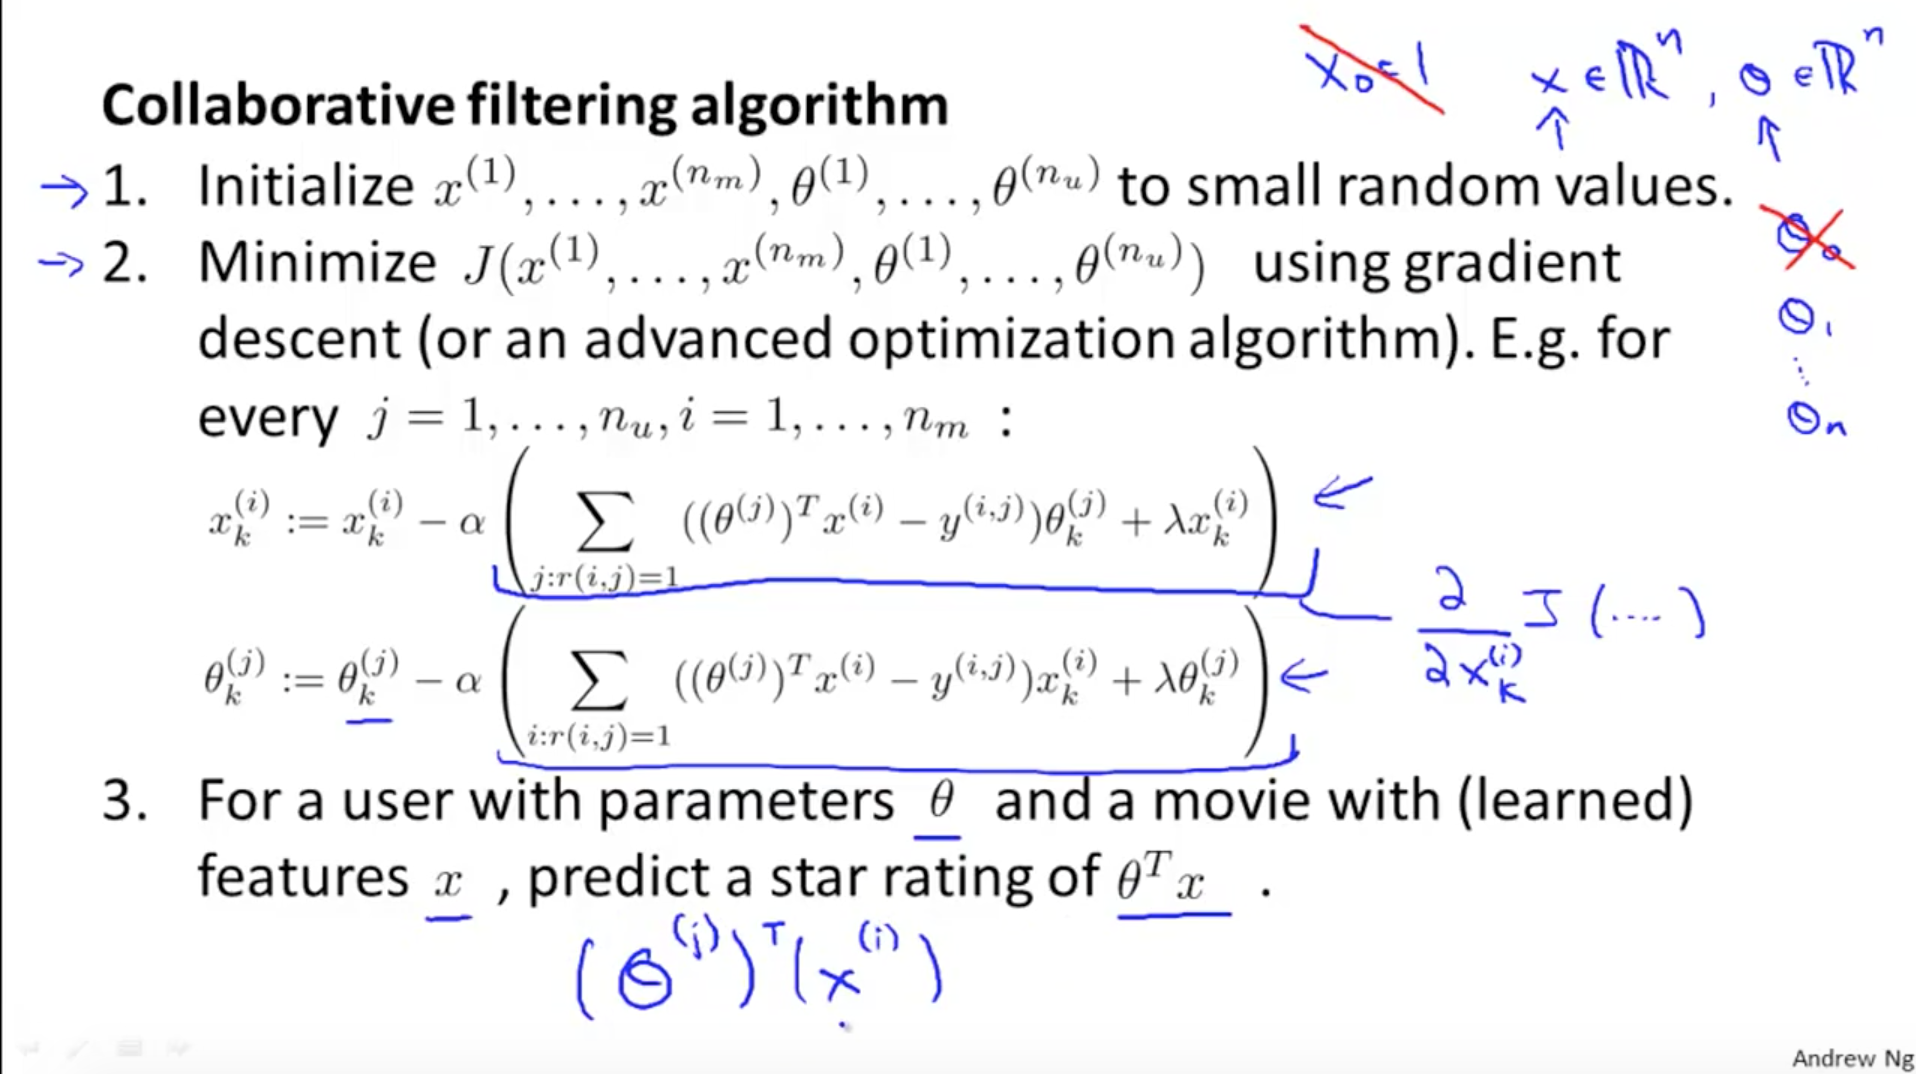
\includegraphics[width= 1.5\textwidth,center]{Collaborative_Filtering_Algorithm.png}
				\caption{What to do}
			\end{figure}
		\end{itemize}
		
	\subsection{Vectorization: Low Rank Matrix Factorization}

		\begin{figure}[ht!]
			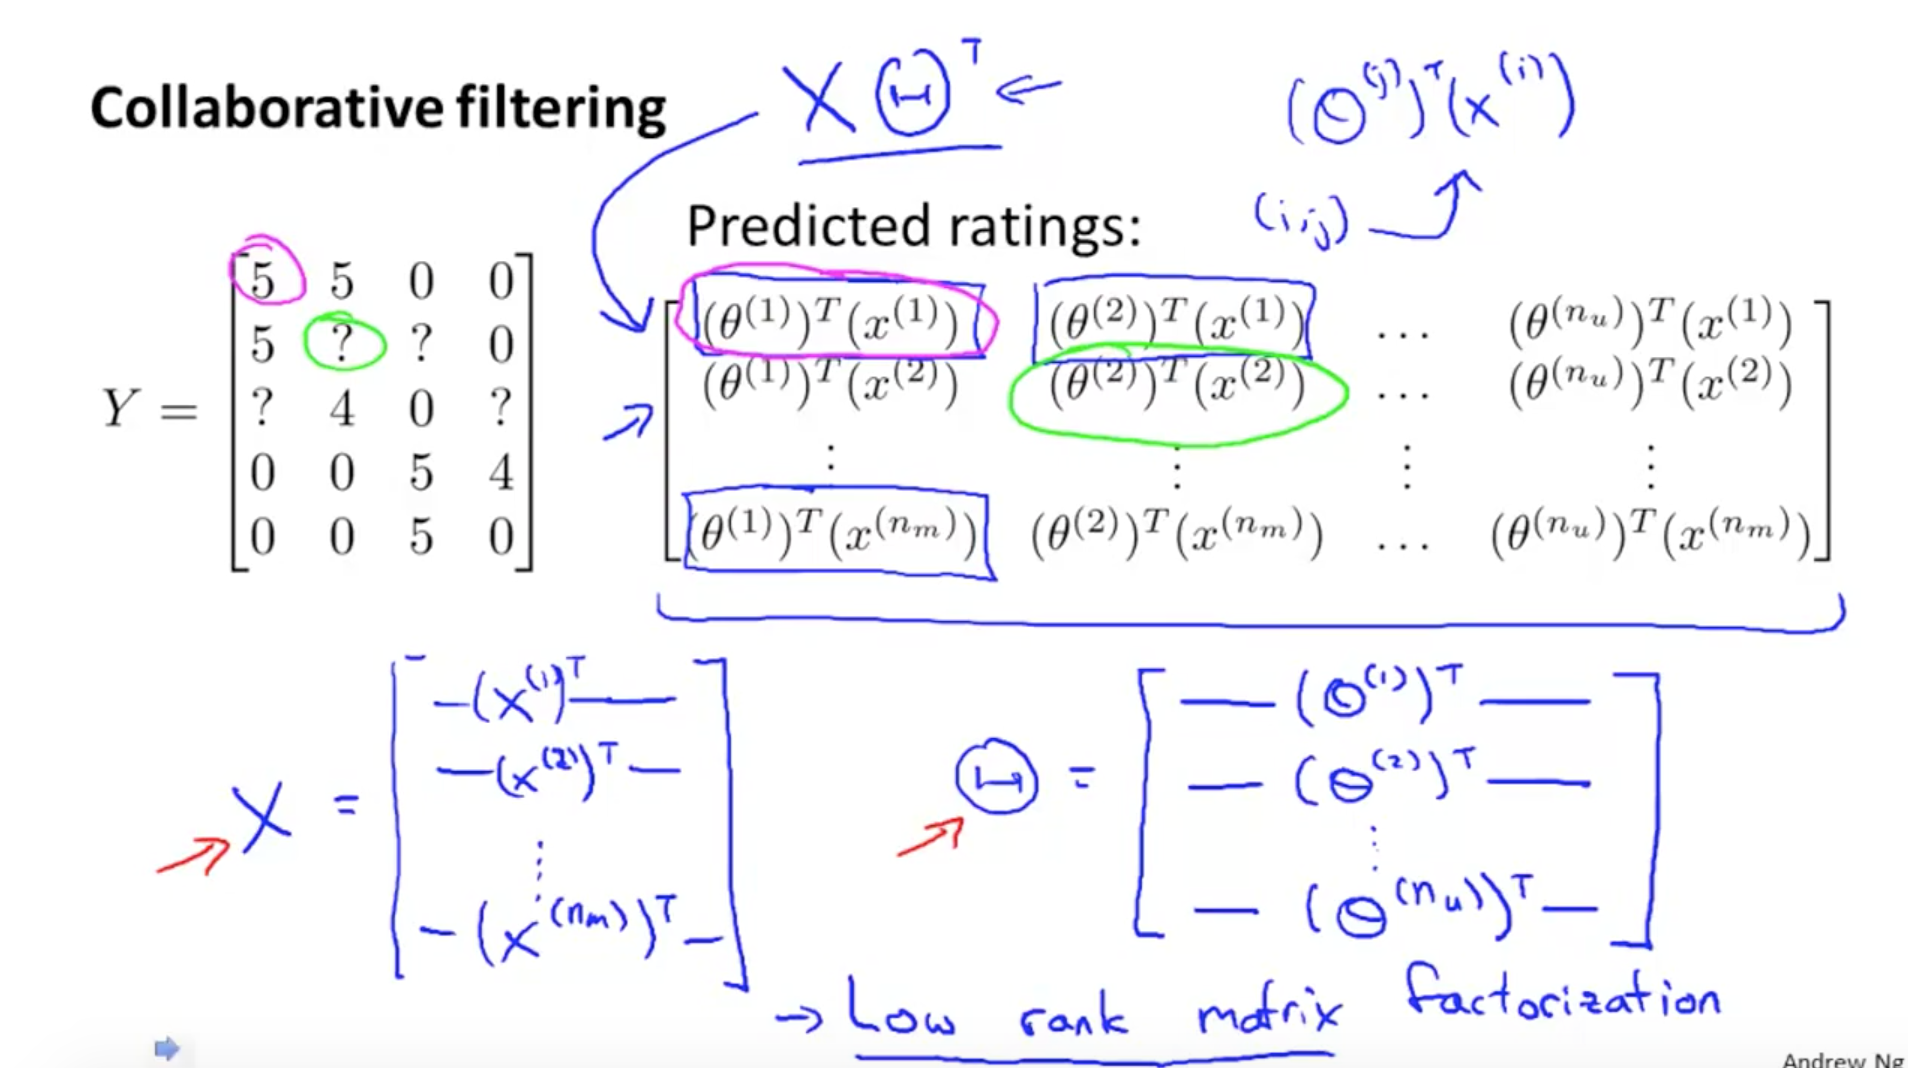
\includegraphics[width= 1.5\textwidth,center]{Collaborative_Filtering.png}
			\caption{Uses Low Rank Matrix Factorization}
		\end{figure}
		\begin{figure}[ht!]
			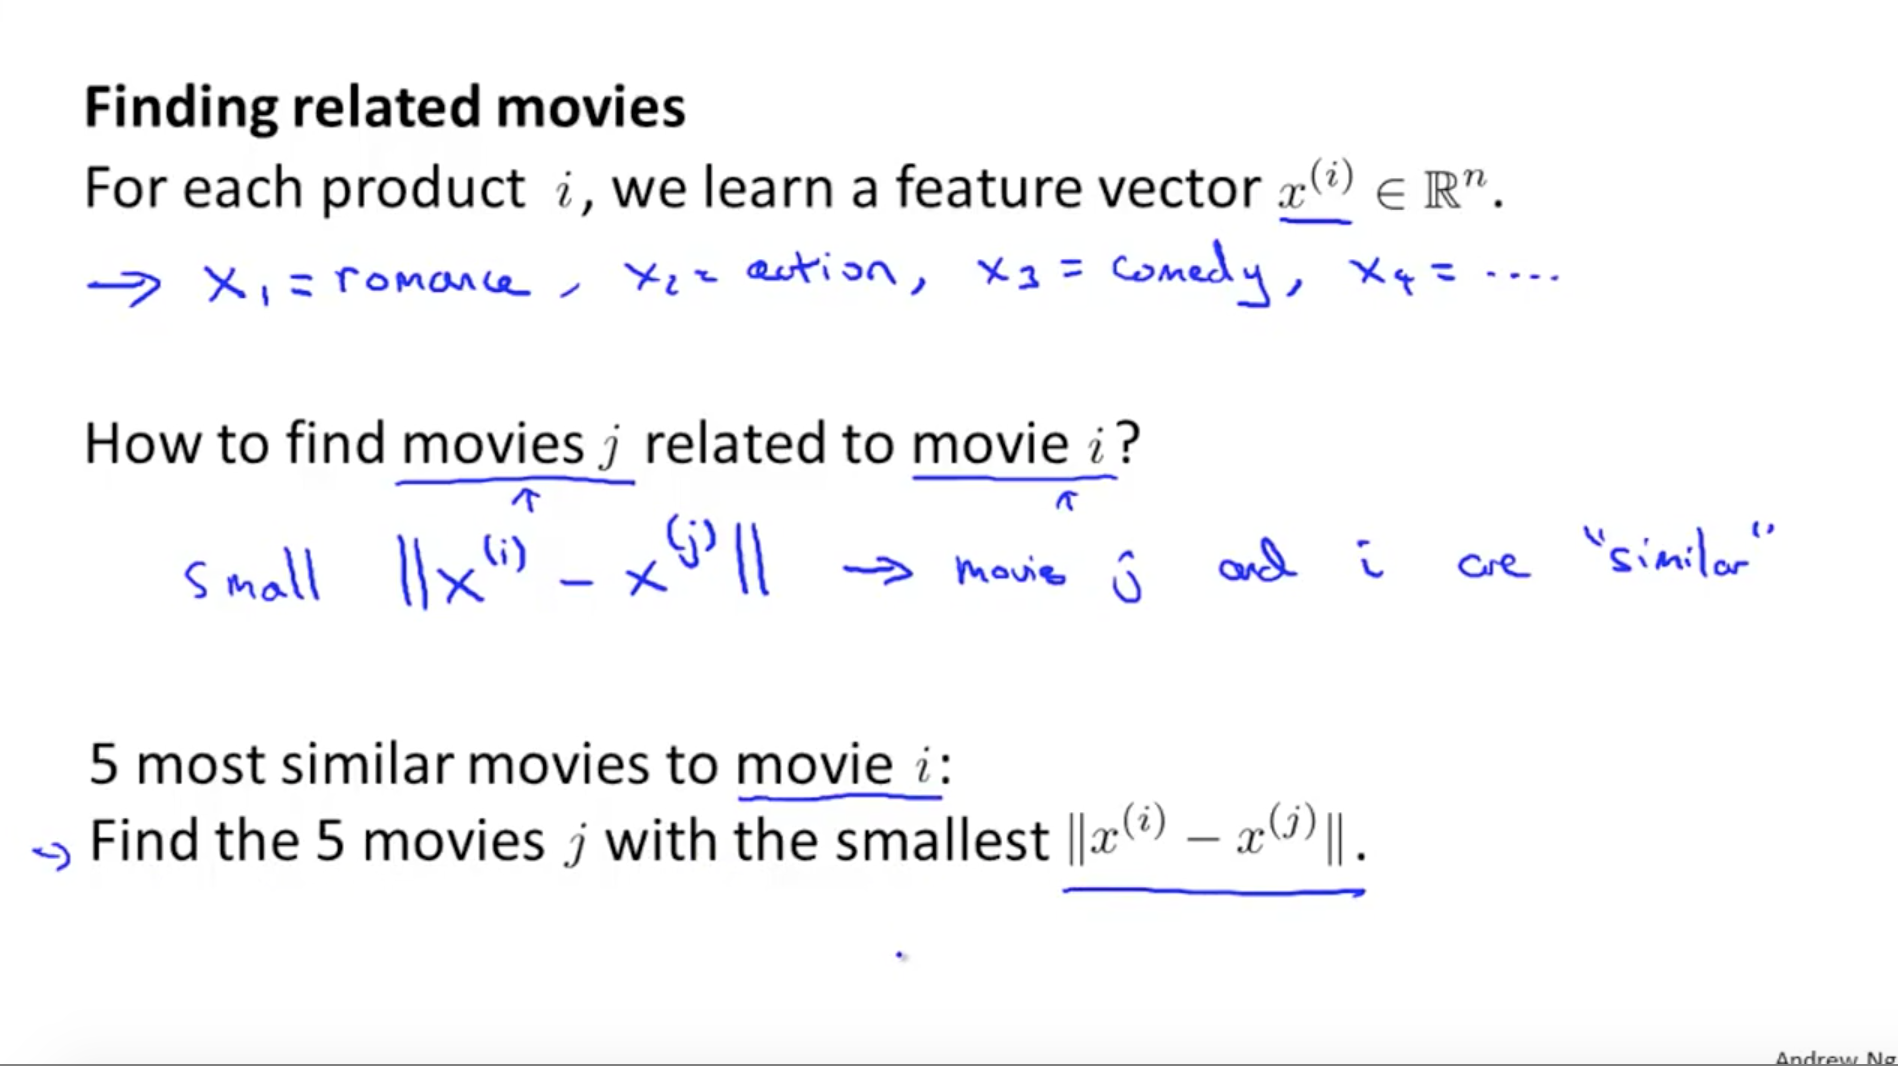
\includegraphics[width= 1.5\textwidth,center]{Finding_Related_Movies.png}
			\caption{How to find related items: check the distance between the two items (since we're dealing with vectors)}
		\end{figure}
		
	\subsection{Implementational Detail: Mean Normalization}
			\begin{figure}[ht!]
				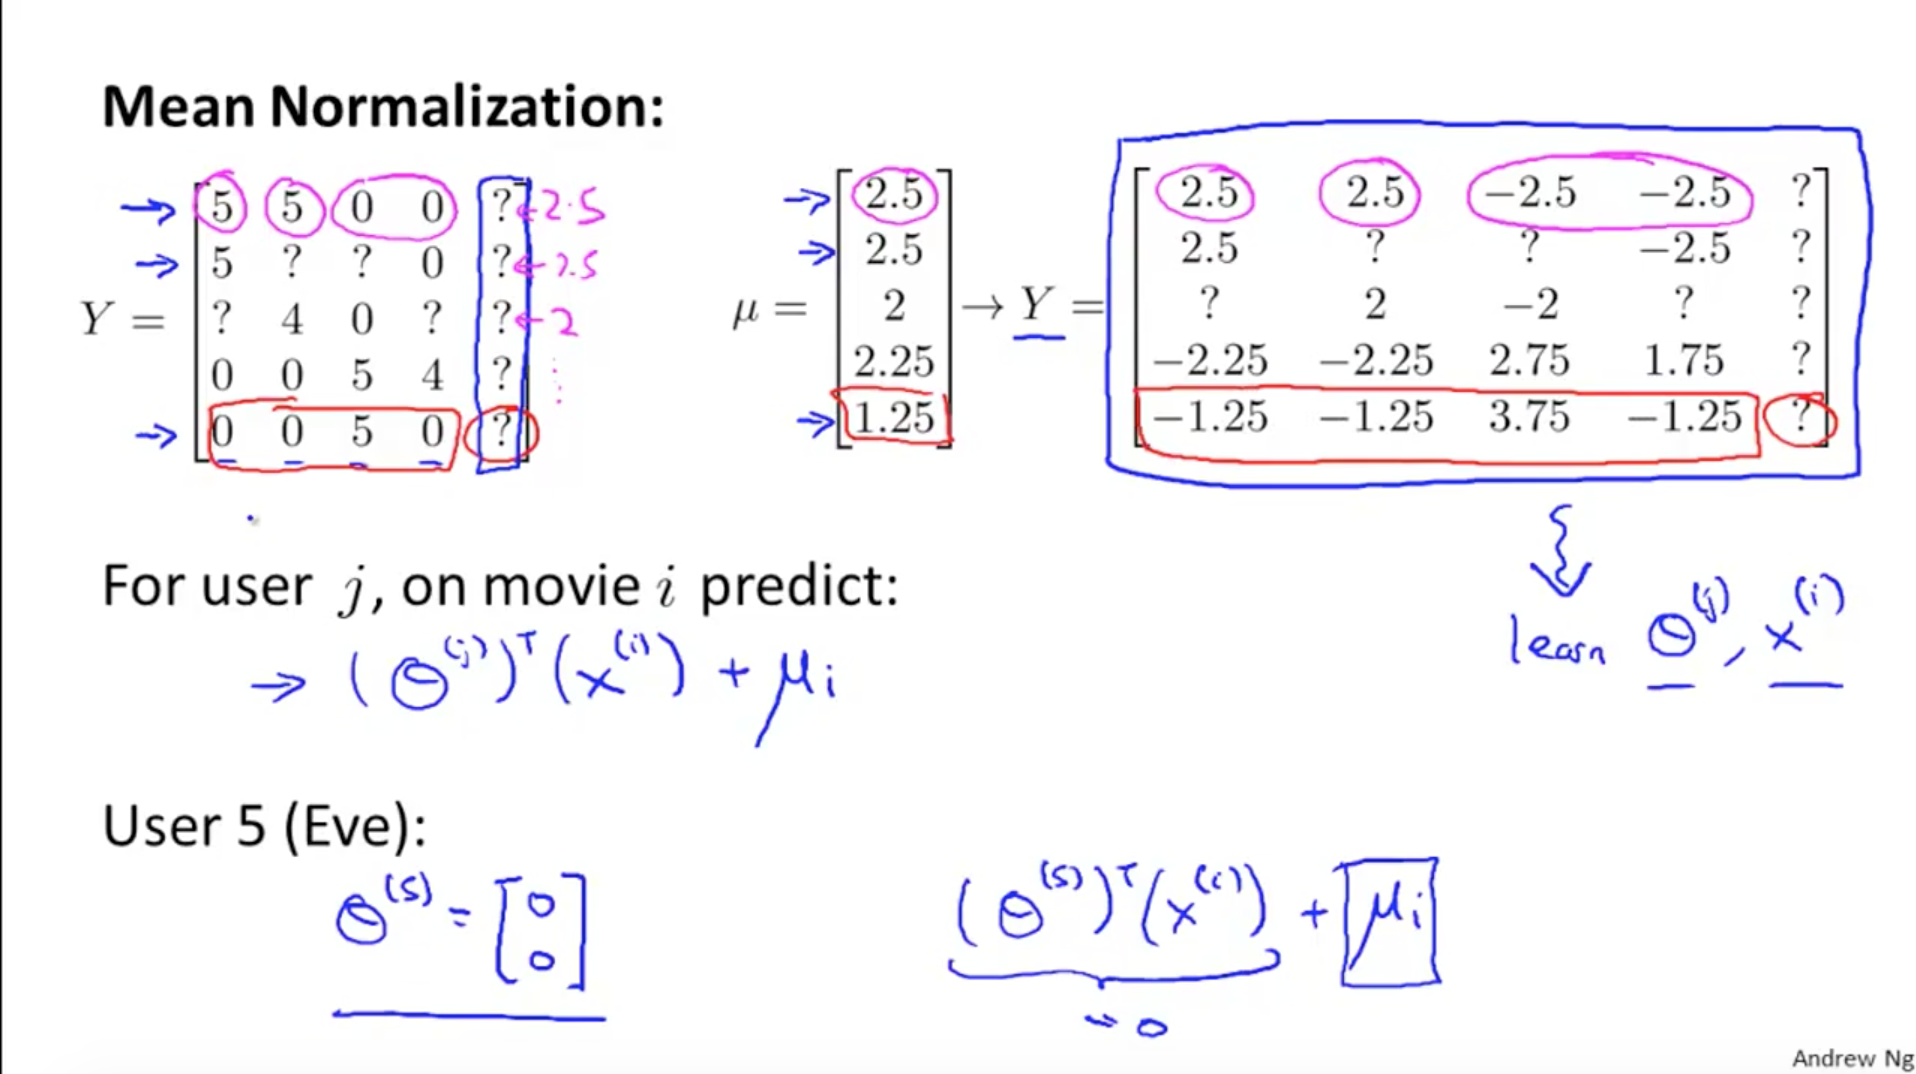
\includegraphics[width= 1.5\textwidth,center]{Mean_Normalization.png}
				\caption{Normalize the means. Helps with recommending movies to a user that has not rated any movies.}
			\end{figure}

\section{Large Scale Machine Learning}

	\subsection{Learning With Large Datasets}
		\begin{itemize}
			\item large data sets are useful for machine learning
			\item but there are issues that arise
			\item one obvious one might be that it takes a large time to perform computations on 100 million examples
			\item But before using large amounts of training examples, check it it's going to help
			\item (plot Jcv and Jtrain as a function of \# on training examples like before, and check if there's high variance first)
			\item (and as before, with high bias, large amounts of bias won't be fixed by large training \#s (can add more neurons or something))
			
		\end{itemize}
		
	\subsection{Stochastic Gradient Descent}
		\begin{itemize}
			\item in normal gradient descent, or "batch" gradient set, we would need to compute the gradient descent for all $m$ training examples (takes time for a large $m$)
			\item now, for large data sets, we use stochastic gradient descent
			\item the steps are:
			\begin{enumerate}
				\item Randomly Shuffle Dataset
				\item Repeat {
					 	for i = 1,...,m {
					 		$\theta_j =\theta_j-\alpha(h_\theta(s^{(i)})-y^{(i)})x_j^{(i)}$	Note: the h-y is the derivative of the cost function
								(for j=0,...,n)
							}
						}
			\end{enumerate}
			\begin{figure}[ht!]
				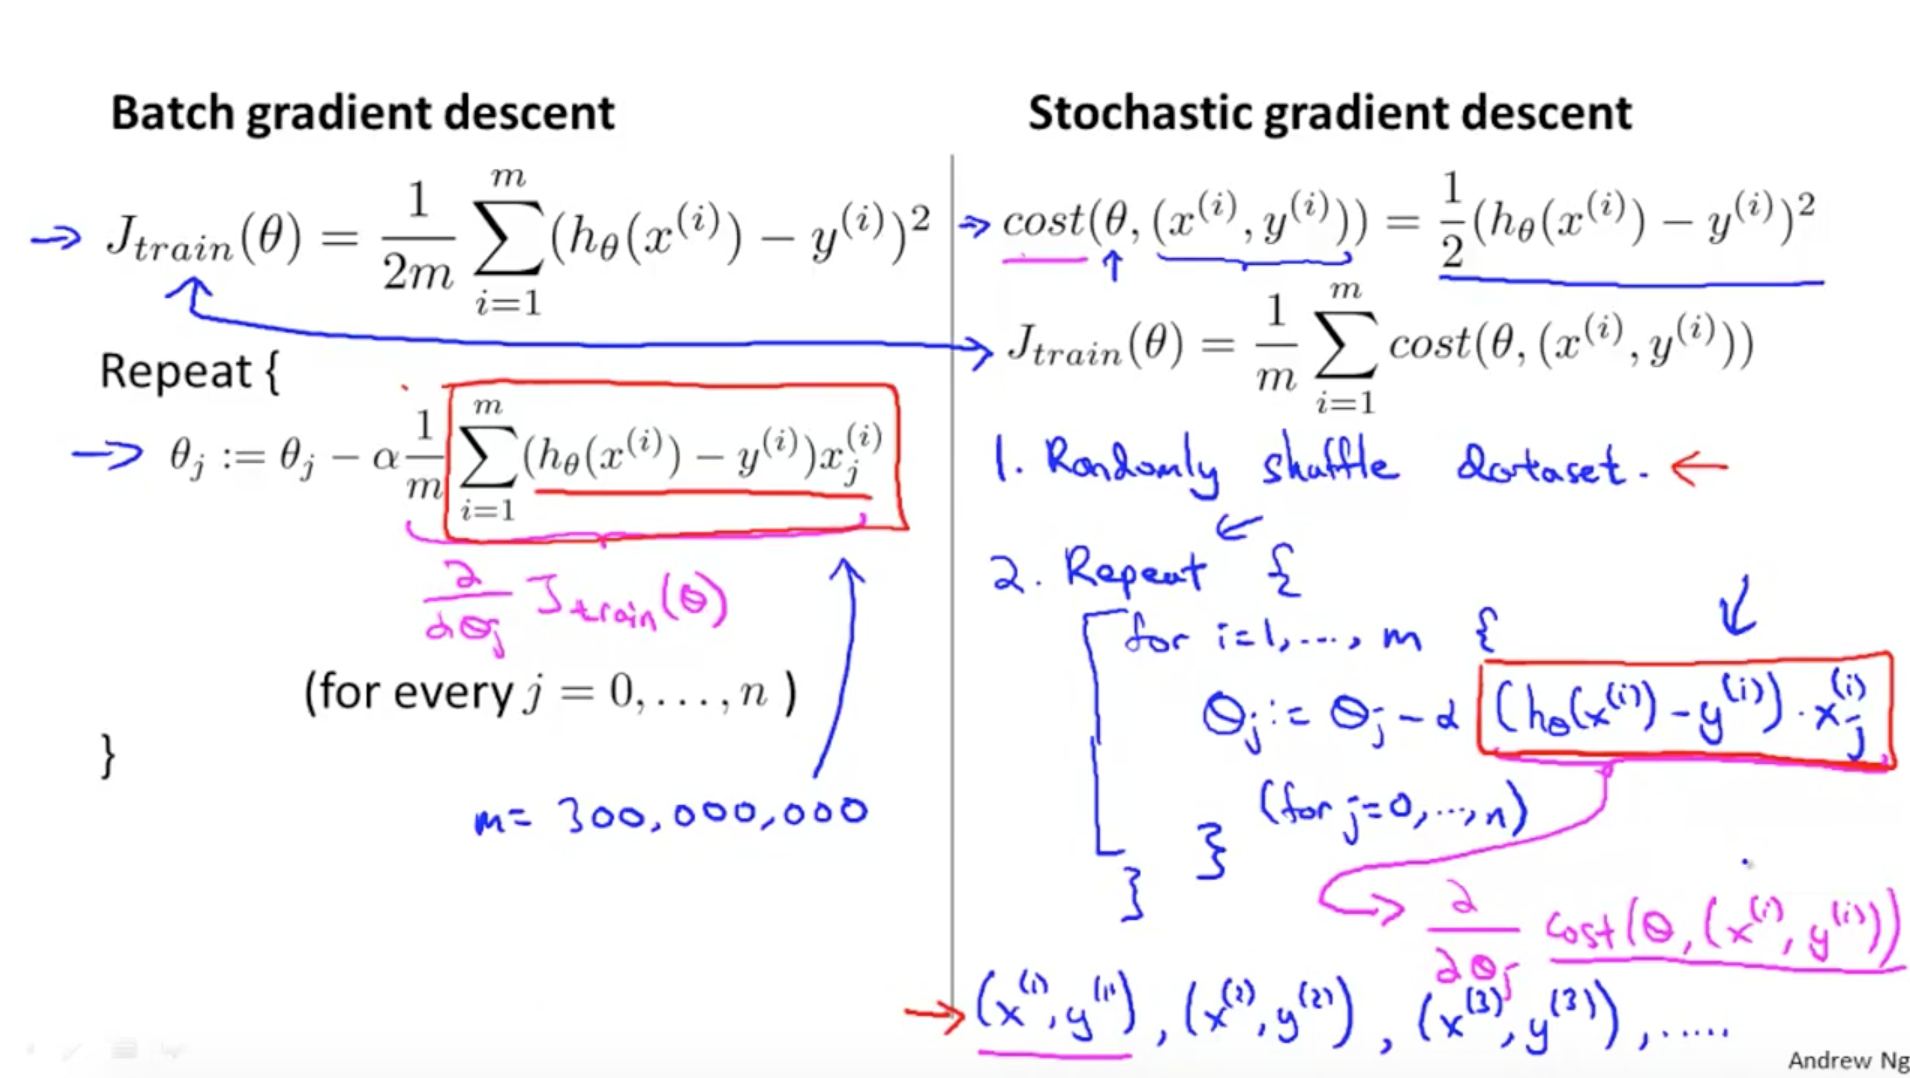
\includegraphics[width= 1.5\textwidth,center]{Stochastic_Grad_Descent.png}
				\caption{The algorithm, and how it compares to normal "Batch" Grad Descent}
			\end{figure}
			\begin{figure}[ht!]
				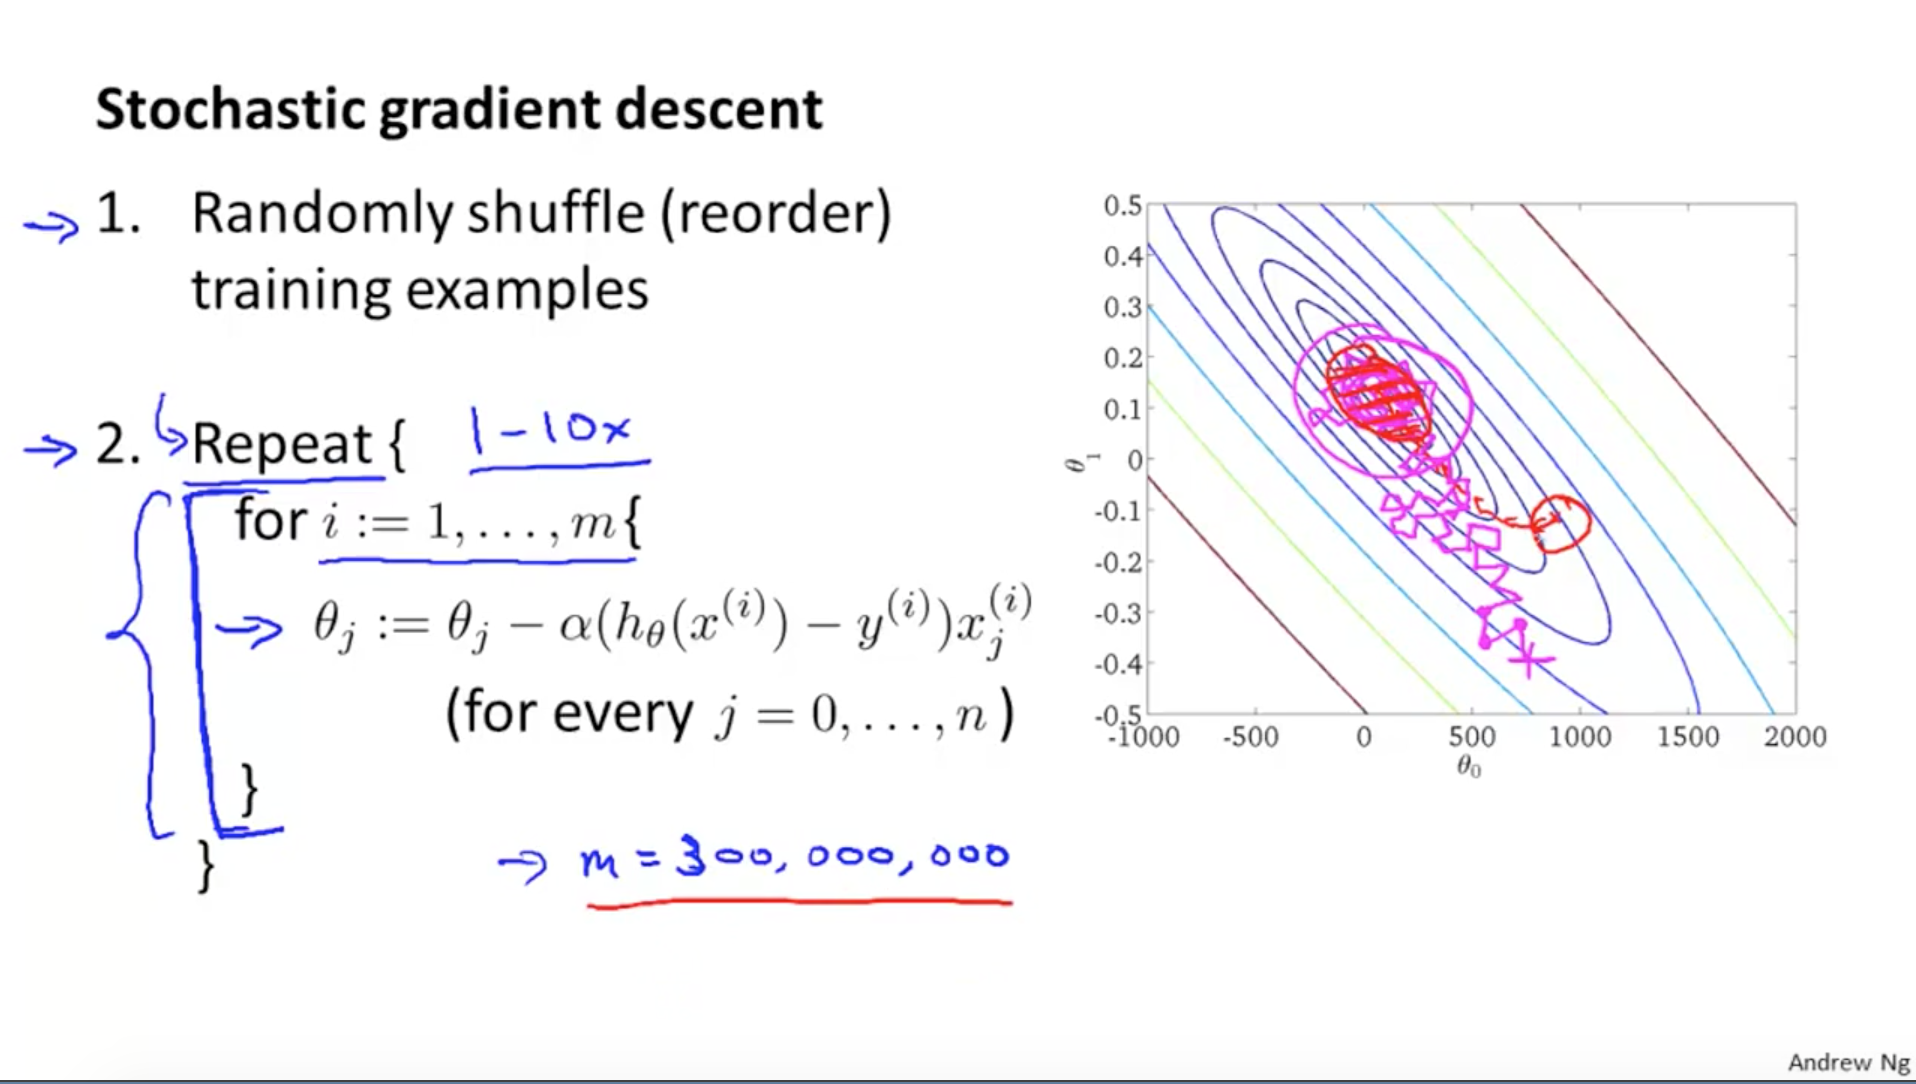
\includegraphics[width= 1.5\textwidth,center]{Stochastic_Grad_Descent_Visualization.png}
				\caption{A visualization.}
			\end{figure}
			\item the algorithm goes through the examples one at a time, and improves theta one at a time to build progress (will finish in one go through of all $m$ examples)
			\item it generally lands near the global minimum, which is good enough
			\item compared to batch gradient descent, this is faster, since after batch takes only one gradient step towards the minimum after computing all $m$ terms, and needs to compute them again to compute it again to take another small step.
		\end{itemize}
	
	\subsection{Mini-Batch Gradient Descent}
		\begin{itemize}
			\item So: Batch grad desc: all $m$ examples
			\item Stochastic grad desc: Use 1 example each iteration
			\item Mini-Batch grad desc: Use $b$ examples each iteration (b = mini-batch size)
			\item Now, this can be faster than Stochastic grad desc because you can use a vectorized approach to calculating those $b$ examples at the same time (some parallel computing, or a good linear algebra library)
		\end{itemize}
		
	\subsection{Stochastic Gradient Descent Convergence}
		\begin{itemize}
			\item we check the cost during learning (calc the cost during the learning)
			\item then, maybe every 1000 iterations, plot the cost (averaged over those 1000 examples)
			\item To try to make the algorithm converge better near the end of the training, you can try to make alpha equal to some constant divided by another constant plus the number of iterations, which will lower alpha as more iterations pass
			
		\end{itemize}
		
	\subsection{Online Learning}
		\begin{itemize}
			\item keep learning from a continuous stream of data (like people online on a shipping website, choosing to use your shipping service)
			\item maybe we would want to try to optimize the price to get the most sales
			\item We could make the site repeat the following forever (while it's on)
			\item -- Get (x,y) corresponding to the user
			\item -- Update theta using (x,y):
			\item -- 	$\theta_j = \theta_j - \alpha(h_{\theta}-y)x_j (j=0,...,n)$
			\item This can adapt to changing user preference since it just keeps getting examples from users that visit the site
			\begin{figure}[ht!]
				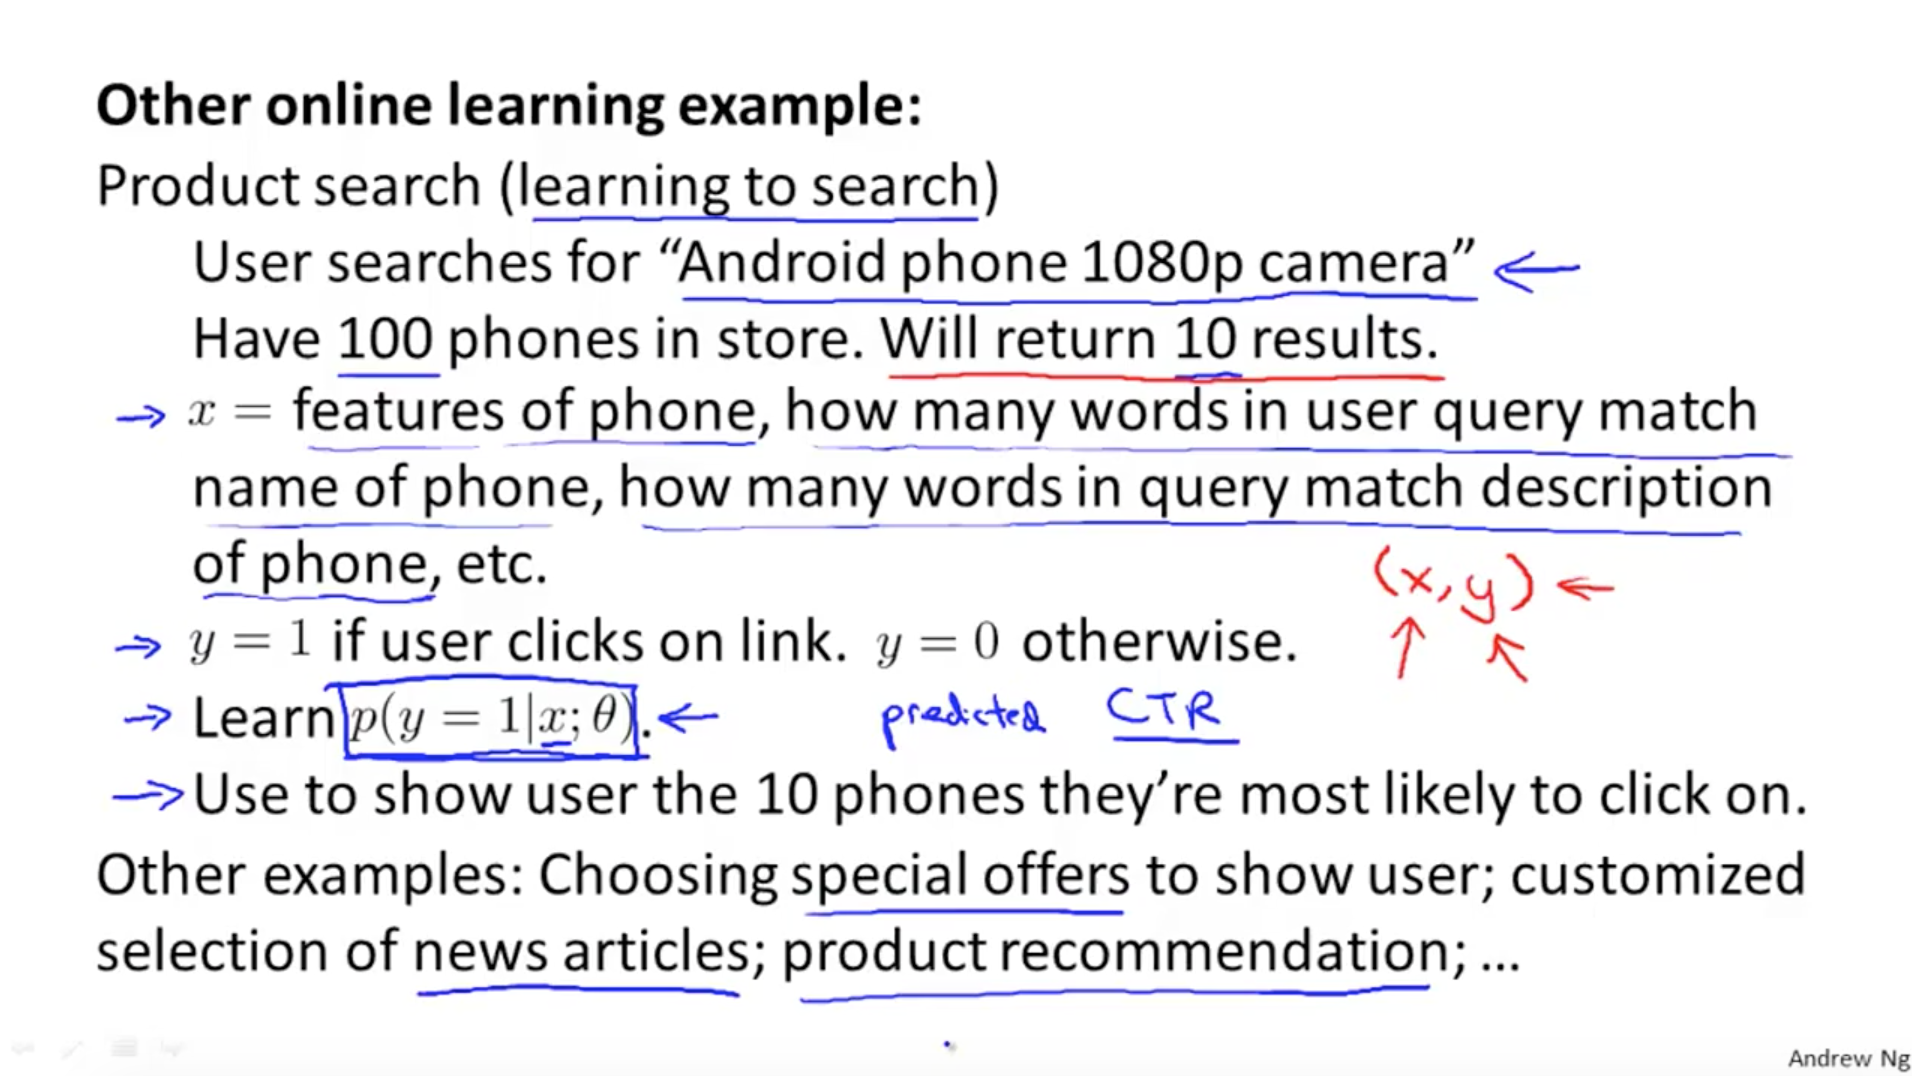
\includegraphics[width= 1.5\textwidth,center]{Online_Learning_Example.png}
				\caption{A good example.}
			\end{figure}
		\end{itemize}
		
	\subsection{Map Reduce and Data Parallelism}
		\begin{itemize}
			\item \emph{Map-reduce}
			\item Ex. we're doing batch grad desc with m = 400.
			\item let's say we have multiple computers, maybe 4 computers
			\item we could have computer 1 use $(x^{(1)},y^{(1)},...,x^{(100)},y^{(100)})$
			\item $temp_j^{(1)} = \sum\limits_{i=1}^{100}(h_{\theta}(x^{(i)})-y^{(i)})x_j^{(i)}$
			\item then comp. 2 use  $(x^{(101)},y^{(101)},...,x^{(200)},y^{(200)})$
			\item $temp_j^{(2)} = \sum\limits_{i=101}^{200}(h_{\theta}(x^{(i)})-y^{(i)})x_j^{(i)}$
			\item and so on and so forth for all 4 machines
			\item so we would get $\theta_j := \theta_j-\alpha\frac{1}{400}\sum\limits_{i=1}^{400}(temp_j^{(1)}+temp_j^{(2)}+temp_j^{(3)}+temp_j^{(4)})$
			\item one thing that might limit it is propagation delay between the computers back to the head computer. but, this would provide a 4x speedup (in theory, in reality, we have some delay between computers)
			\item -----------------------------------------------------------------
			\item So, to use Map-reduce(distributed computing) and summation over training sets
			\item just distribute the summation/vectorized program over multiple computers (or CORES!)
			\item with this, network latency/propagation delay is less of an issue since the components are in the same machine
			\item (A good open source implementation of Map-reduce is Hadoop, check it out)
		\end{itemize}
		
\section{Applications of Machine Learning}
	\subsection{Problem Description and Pipeline}
		\begin{itemize}
			\item \emph{The Photo OCR problem}: get computers to read text from images
			\item the Photo OCR pipeline, given an image to work on
			\begin{enumerate}
				\item Text detection - detect where the text is
				\item Character segmentation - separate the characters
				\item Character classification - figure out what each character is
			\end{enumerate}
			\item we can made different modules to do each step. the first module would call the next one when it is done, and so one
		\end{itemize}
		
	\subsection{Sliding Windows}
		\begin{itemize}
			\item going back to detecting things, like pedestrians in a picture, how do we detect things?
			\item we could have general size for the image we're searching for, and take the image, and check a box of the size we decided on, and slide it a few pixels over and check with our classifier.
			\item we keep doing this with these "\emph{image patches}" of the size we decided on
			\item if the items are at different distances, we would need to check different sizes of rectangles due to the different distances the items are away
			\item the result might be something like a matrix of probabilities of where text might be. to "clean it up", we could run an algorithm to see if there are other high probability areas to the left or right, and if there are, we would make this area a high probability area.
			\begin{figure}[ht!]
				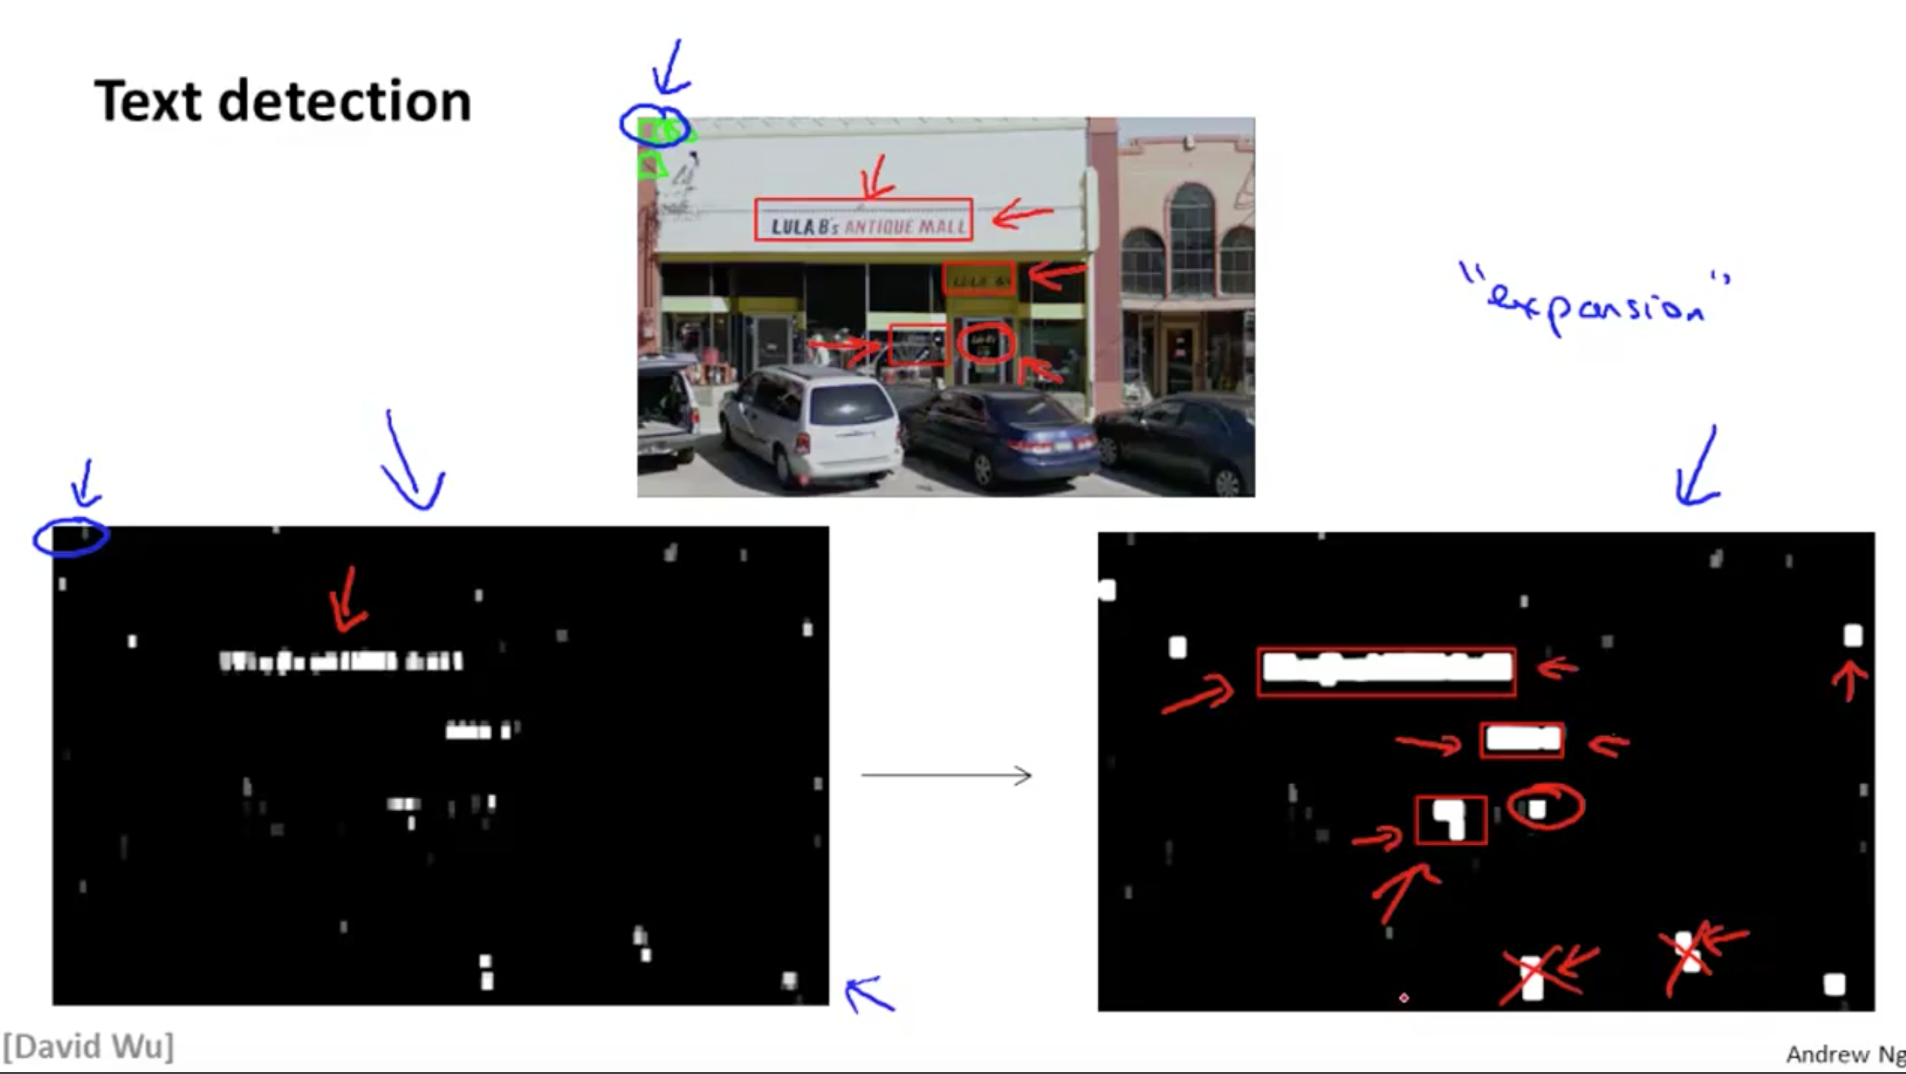
\includegraphics[width= 1.5\textwidth,center]{Text_Detect_Ex.png}
				\caption{Ex. on what detecting text might look like}
			\end{figure}
			\item Now, for character segmentation, we try to check for a split between characters
			\item and again, we do use the sliding window technique, and run our classifier on each window
			
		\end{itemize}
	
	\subsection{Getting Lots of Data and Artificial Data}
		\begin{itemize}
			\item \emph{Artificial data synthesis for photo OCR}
			\item \emph{Ex. 1} make artificial data of recognizing characters
			\item just take different fonts, make some text/characters, and then distort them.
			\item you can also take items from your character training set, you could make different distortions and have those as different examples. But make sure your distortions are reasonable
			\item \emph{Ex. 2 synthesizing data by introducing distortions: Speech Recognition}
			\item introduce some small distortions into your speech examples
			\item \textbf{NOTE:} Just adding random noise usually DOES NOT HELP (like adding random gaussian dots on a character image)
			\item Note: make sure you have a low bias classifier before trying to do these things.
			\item just plot learning curves (cost vs \# of training examples)
			\item to lower bias, you can try adding more features/\# of hidden units in a neural net until you have a low bias classifier
			\item Note: ask if it's possible to get 10x as much data you currently have (sometimes it's easy for them, so ask)
			\item - then if needed, maybe try adding artificial data
			\item - maybe try collecting/labeling data yourself (try to figure out how long this would take, since this can take a few days, but it's only a few days)
			\item - "Crowd source" (e.g. Amazon Mechanical Turk (very popular at the moment))
			
		\end{itemize}
		
	\subsection{Ceiling Analysis: What Part of the Pipeline to Work on Next}
		\begin{itemize}
			\item \emph{Ceiling Analysis}
			\item we'll use the text detection example to explain
			\item Now: Which part of the pipeline should be focus on the most?
			\item We check each components and their accuracy
			\item We could check the overall system and it's accuracy
			\item Then, we could manually give the next part a perfect data set we made, so that when we check the next part's accuracy, we have an accurate way to check the accuracy
			\item recap: feed in our perfect results we manually made to evaluate the true accuracy of each module, without being affected by the previous module's accuracy
			\item a simple work flow/pipeline might be:
			\begin{enumerate}
				\item Preprocessing (remove background)
				\item Face detection
				\begin{itemize}
					\item Eyes segmentation
					\item Nose segmentation
					\item Mouth segmentation
				\end{itemize}
				\item Logistic regression
			\end{enumerate}
			\item then we feed in out perfect data to each component and check each part's algorithm
			\item True Story: some specific scientists spent 18 months trying to improve the preprocessing, but then came to realise that it didn't really have much effect on the accuracy of the system
			\item Moral: DO CEILING ANALYSIS TO MAKE SURE WHAT YOU ARE DOING IS WORTH IT
			\begin{figure}[ht!]
				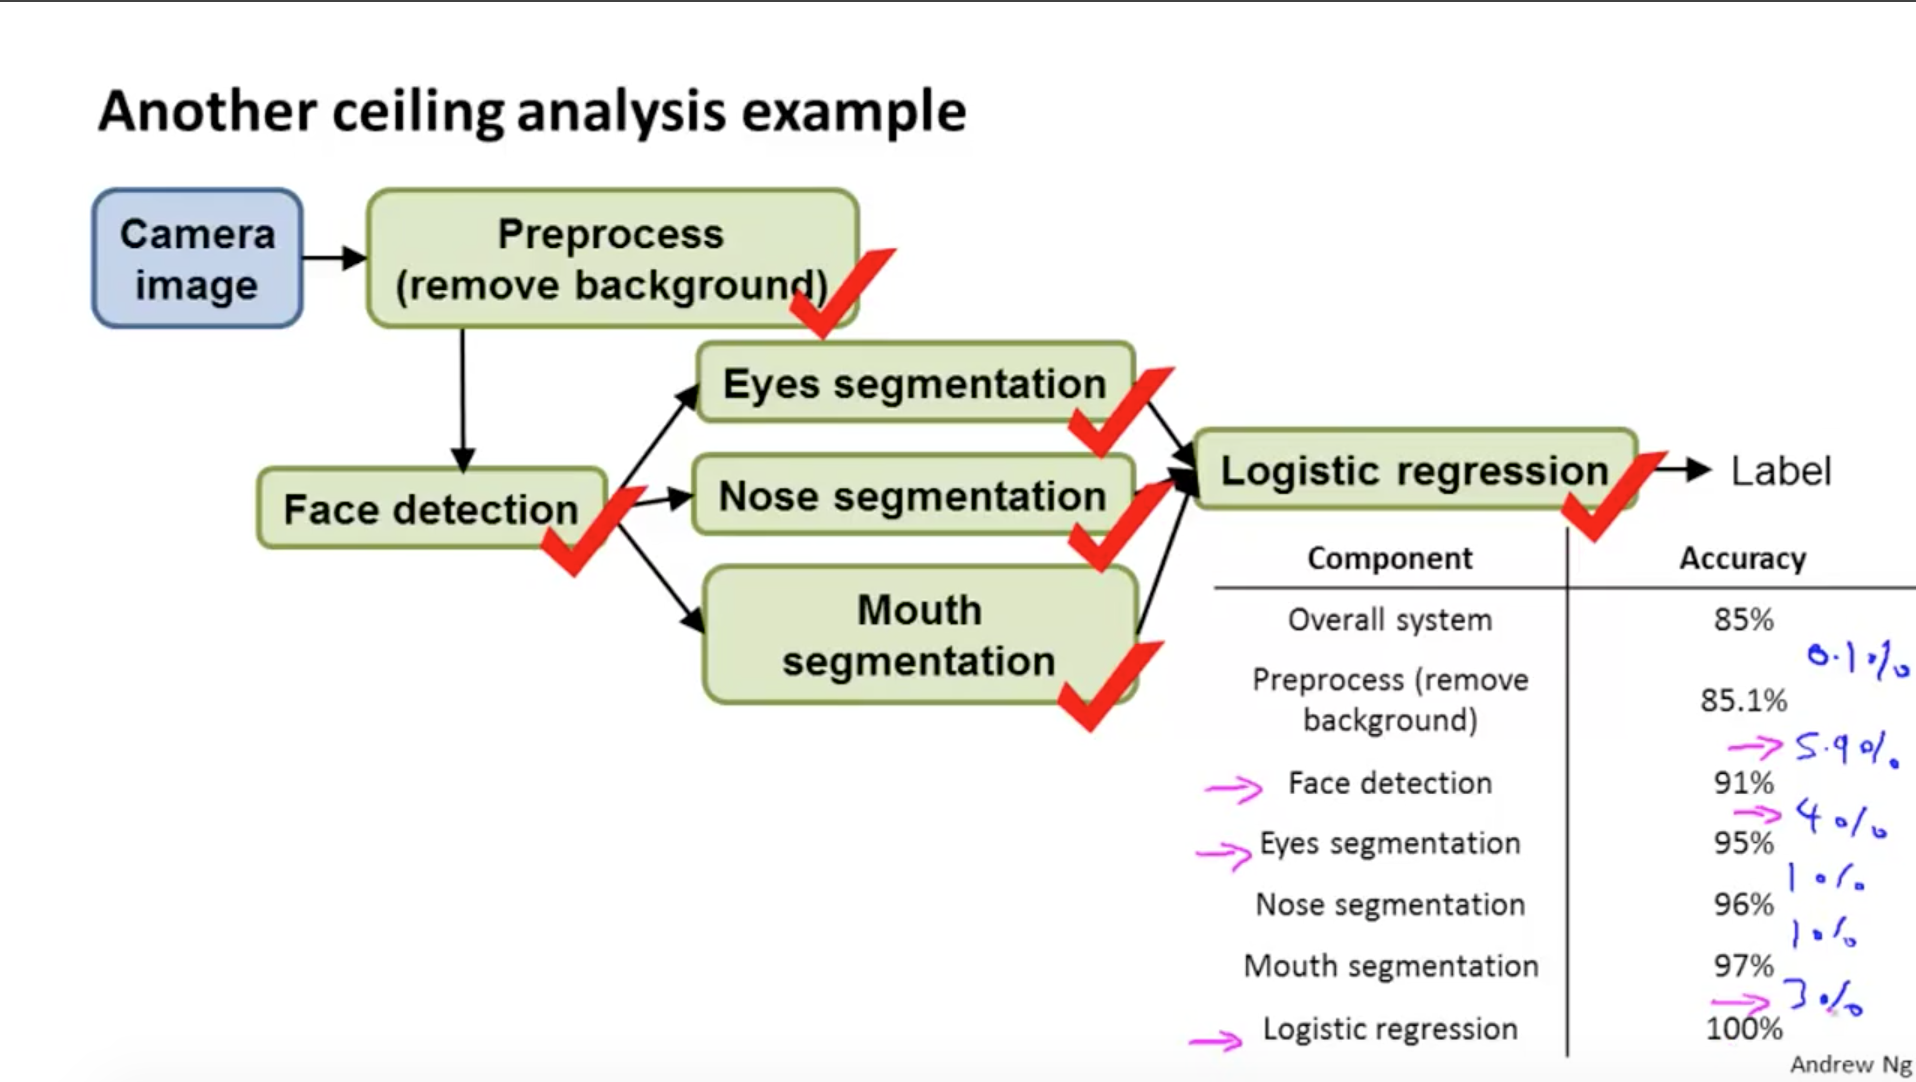
\includegraphics[width= 1.5\textwidth,center]{Ceiling_Analysis_Example.png}
				\caption{A good example.}
			\end{figure}
		\end{itemize}
\end{document}